%
% METU Institute of Natural and Applied Sciences Thesis example
%
% Edited and Commented by Utku Erdoğdu 2012
%
% Please read the explanations so that you can customize the document
%
% Files needed by this document:
% metu.cls
% metu11.def (if you will use 11pt fonts)
% metu12.def (if you will use 12pt fonts)
% metu10.def (if you will use 10pt fonts)
%
% Possible Options Here:
%
% oneandhalf, double, single : Line spacing used in the thesis. Default and institute preference is
% single.
%
% 10pt, 11pt, 12pt : Font size Default is 10pt, which is institue choice.
%
% pntr, pntc, pnbt : Page number position. Options are top center, top right or bottom. Default and
% institute preference is page numbers at bottom. When page numbers are at the top bottom margins
% are skewed.
%
% chaproman, chaparabic: Chapter numbering format. Options are roman numbers and arabic numbers.
% Default is roman, institute prefers arabic
%
% oneside, twoside : Printing style. Default is twoside, which is institute choice. In this style
% chapters begin from odd numbered pages.
%
% tr, eng : Document language. This is useful if you want to translate your thesis into
% Turkish. Then you give the option tr and use \ifturkish. . .\else. . .\fi  whenever you want
% to do something only for Turkish or only for English. Default is eng.
% IMPORTANT!! : For official institute documents you should not use this option.
% The Turkish format is only supplied for custom translations.
%
% ceng,aee,arme.. : You can use the abbreviated form of your department here and there is no further need to
% define the department name below. If your department name is not among the below list of defined
% departments, you should use \department and \turkishdepartment macros to define the name of your
% department.
%
% Defined Departments and Abbreviations:
% --------------------------------------
% Computer Engineering : ceng
% Aerospace Engineering : aee
% Archaeometry : arme
% Architecture : arch
% Biochemistry : bch
% Biology : biol
% Biomedical Engineering : bme
% Biotechnology : btec
% Building Science : bs
% Cement Engineering : ceme
% Chemical Engineering : che
% Chemistry : chem
% City and Regional Planning : crp
% City Planning : cp
% Civil Engineering : ce
% Computational Design and Fabrication Technologies in Architecture : arcd
% Computer Education and Instructional Technology : cte
% Design Research for Interaction : iddi
% Earthquake Studies : eqs
% Earth System Science : ess
% Electrical and Electronics Engineering : ee
% Engineering Management : em
% Engineering Sciences : es
% Environmental Engineering : enve
% Food Engineering : fde
% Geodetics - Geographical Information Technologies : ggit
% Geological Engineering : geoe
% Hydrosystems Engineering : he
% Industrial Design : id
% Industrial Engineering : ie
% Mathematics : math
% Mechanical Engineering : mech
% Metallurgical and Materials Engineering : mete
% Micro and Nanotechnology : mnt
% Mining Engineering : mine
% Operational Research : or
% Petroleum and Natural Gas Engineering : pete
% Physics : phys
% Polymer Science and Technology : pst
% Regional Planning : rp
% Restoration : rest
% Secondary Science and Mathematics Education : ssme
% Software Engineering : se
% Statistics : stat
% Structural Mechanics : st
%
% phd, ms : Degree Received. Ph.D. or M.S. Default is M.S.
%
% End of Options
\documentclass[11pt,single,chaparabic,ceng,ms,eng]{metu}
% You can delete next line If your thesis does not have an appendix
\usepackage{appendix}

%
% Use your latex packages here
\usepackage{graphicx}
\usepackage{epstopdf}
\usepackage{colortbl}
\usepackage{array}
\usepackage{amsmath}
\usepackage{txfonts}
\usepackage{float}
\usepackage{subfig}
\usepackage{rotating}
\usepackage{tikz}
\usepackage{tabularx}
\usepackage{amssymb}
\usepackage{multirow}
\usepackage{slashbox}
\usepackage{verbatim}
\usepackage{hhline}
\definecolor{Gray}{gray}{0.85}
\definecolor{LightCyan}{rgb}{0.88,1,1}
% End of Latex Packages
%
% Any personal Latex definition, decleration, etc.


% End of personal stuff
%
% Personal Information
% ----------------------------
%
% Please check this part and fill in information about your thesis
%
% Name and Surname
\author{Saber HafezQorani}
% Thesis Title English and Turkish
\title{MODELING THE COMBINED EFFECT OF RNA-BINDING PROTEINS AND MICRORNAS IN POST-TRANSCRIPTIONAL REGULATION}
\turkishtitle{TRANSKRIPSIYON-SONRASI KONTROLDE RNA'YA BAGLANAN PROTEIN'LER VE MIKRORNA'LARIN ETKİSİNİN BİRLİKTE MODELLENMESİ}
% Department : English and Turkish
%
% Some of the departments are pre-defined, you need not redeclare them. You can use them by just
% giving an option to \documentclass. See documentation for options above. If you will define your
% department here do not use ``Department'' or ``Bölümü'' words.
%\department{Computer Engineering}
%\turkishdepartment{Bilgisayar Mühendisliği}
%
%
% Date : You should indicate the month of your thesis defence in English.
% Default is this month
%
\date{September 2015}
%
% Approval Page Details
% --------------------------
% For each command you can give the title as optional parameter enclosed in [ ]
% This also handles the Turkish titles if you're planning to produce Turkish version of the
% document. If you'll hard code the title, you need to use turkish version of each command after
% the command itself
%
% prof : Prof. Dr.
% assocprof : Assoc. Prof. Dr.
% assistprof : Assist. Prof. Dr.
% dr : Dr.
%
% Director of Institute
\director[prof]{Nazife Baykal}
% Head of Department
\headofdept[assocprof]{Yeşim Aydın Son}
%
% Supervisor : English and Turkish
\supervisor[assocprof]{Yeşim Aydın Son}
% \turkishsupervisor{  } %if you will hard-code the academic title
%
% Affiliation of Supervisor in English and possibly in Turkish
\departmentofsupervisor{Health Informatics, METU}
% Co Supervisor if Any : English and Turkish
% You can just delete the next lines if you don't have a co-supervisor
\cosupervisor[assistprof]{Hilal Kazan}
% \turkishcosupervisor{Prof. Dr. Reda Alhajj} %if you will hard-code the academic title
% Affiliation of Co-Supervisor
% You can just delete the next line if you don't have a co-supervisor
\departmentofcosupervisor{Computer Engineering, Antalya International University}
%
% Committee Members
% In general members are sorted according to their academic titles
%
% Proffesors (1)
% Associate Professors (2)
% Assistant Professors (3)
% Other (4)
%
% IMPORTANT:  All affiliatons should fit in a single line
% If affiliation line is broken into two lines you should shorten the affiliation by using
% abbrevations or any other means
%
% First committee member should be the chair of examining committee
% Typically the chair is one of the highest ranked committee members
% Ask your supervisor if you are not sure
\committeememberi[]{Aybar Can Acar}
% \turkishcommitteememberi{Prof. Varol Akman} % if you will hard-code the academic title
\affiliationi{Health Informatics, METU}
% Second committee member is always your supervisor
\committeememberii{Yeşim Aydın Son}
\affiliationii{Health Informatics, METU}
% If you are an M.Sc. student and your Co-Supervisor is in your
% examination committee, then third committee member is always your co-supervisor
%
% IMPORTANT: If you are Ph.D. student your co-supervisor can not be in your
% examination committee.
\committeememberiii{Hilal Kazan}
\affiliationiii{Computer Engineering, AIU}
% Fourth committee member
\committeememberiv{Tolga Can}
\affiliationiv{Computer Engineering, METU}
% Fifth committee member
\committeememberv{Bala Gür Dedeoğlu}
\affiliationv{Biotechnology Institute, Ankara University}
%
% Keywords : English & Turkish, Comma seperated
\keywords{Post-transcriptional regulation, RNA-binding proteins, MicroRNAs, RNA secondary structure, mRNA stability}
\anahtarklm{Transkripsiyon-sonrası kontrol, RNA'ya bağlanan protein, MikroRNA, RNA'ın ikincil yapısı, gen stabilitesi}
%
% Abstract in English
%
\abstract{Post-transcriptional regulation (PTR) controls the gene expression between transcription and translation. Regulation at this level is carried out by the interactions of trans-acting RNA-binding proteins (RBPs) and microRNAs (miRNAs) with cis-regulatory elements in mRNA. Majority of previous work have focused on the effect of a single factor independent of other co-factors bound to the same mRNA. However, recent studies have shown that RBPs and miRNAs can act in cooperation or competition with each other. In this thesis, we mapped the binding sites of both RBPs and miRNAs on human 3’UTRs, and utilized this collection of binding sites to better understand PTR networks. We first focused on several RBPs and assessed how accessibility and conservation differ between experimentally supported sites and other sites that are only computationally predicted. We then investigated the competitive effects of other factors on HuR binding and the resulting transcript abundance change upon HuR depletion. Next, we characterized the potential interactions between the factors by finding those pairs of factors with co-occurrence of motifs higher than expected by chance. Our results show that PUM1 and PUM2 have potential cooperative interactions with miRNAs. Finally, we used logistic regression with features compiled from the counts of sites of factors and dinucleotide frequency to accurately predict the stability and steady-state abundance of mRNAs. Altogether, results of this thesis suggest that studies of PTR must consider the effect of both RBPs and miRNAs, and their interactions.}
%
% Turkish Abstract
%
\oz{Transkripsiyon-sonrası kontrol (TSK), gen ifadesinin transkripsiyon ile translasyon arasındaki adımlarını kontrol eder. Bu adımların kontrolü RNA'ya bağlanan protein (RBP) ve mikroRNA'ların (miRNA) mesajcı RNA'lardaki (mRNA) hedef noktalarına bağlanmaları sayesinde gerçekleştirilir. Şu ana kadar yapılan çalışmaların büyük çoğunluğunda tek bir RBP ya da tek bir miRNA aynı mRNA'ya bağlanan diğer faktörlerden bağımsız olarak incelenmiştir. Ancak, son çalışmalar RBP ve miRNA'ların birbirleriyle işbirliği ya da rekabet ilişkileri içerisinde olduklarını göstermiştir. Bu tezde, son gelişmelere paralel olarak insan 3'UTR'ları üzerindeki hem RBP, hem de miRNA bağlanma noktalarını belirledik. İlk olarak, üzerinde çalışılmış RBP'lerin deneysel yöntemlerle bulunan bağlanma noktaları ile işlemsel yöntemlerle tahmin edilmiş bağlanma noktalarını RNA'nın ikincil yapısı ve evrimsel korunum bakımından farklı olduğunu gösterdik. Daha sonra, HuR adlı RBP için var olan susturulma sonrası mRNA ifade değişimi verilerini kullanarak diğer faktörlerin HuR'la olan rekabetçi ilişkilerini araştırdık. Ayrıca, iki faktörün (RBP ya da miRNA) bağlanma noktalarının beraber görülme sıklığını hesaplayarak potansiyel işbirliği ilişkilerini inceledik. Bu analiz sonucunda PUM1 ve PUM2 RBP'lerinin miRNA'larla işbirliği içerisinde olduğunu gözlemledik. Son olarak, faktör bağlanma sayıları ve dinükleotid frekansı gibi öznitelikleri bağlanım modeliyle kullanarak gen ifadesi ve stabilitesini yüksek bir doğruluk payıyla tahmin ettik. Elde ettiğimiz sonuçlar transkripsiyon-sonrası kontrol ile ilgili mekanizmaları daha iyi anlamak için RBP'lerin, miRNA'ların ve ayrıca aralarındaki ilişkilerin de göz önünde bulundurulması gerektiğine işaret etmektedir.}
%
% Dedication
\dedication{Dedicated to my family and wife.}
%
%
% Acknowledgements
\acknowledgments{
I would like to express my gratitude to my co-supervisor Assist. Prof. Dr. Hilal Kazan whose expertise, understanding, and patience, added considerably to my graduate experience. It was a great honor to work with her for the last two years and our cooperation influenced my academical view in a great scale. I also would like to thank Assoc. Prof. Dr. Yeşim Aydın Son for her support of my thesis work.

This project is supported by TÜBİTAK (Project No: #113E159). I worked on this project along with my colleague, Atefeh Lafzi, under supervision of Assist. Prof. Dr. Hilal Kazan for the previous two years. Our work also accepted as poster and short communication at several conferences including ISMB 2014 (22nd Annual International Conference on Intelligent Systems and Molecular Biology), MIE 2014 (The 25th International Congress of the European Federation for Medical Informatics), and ECCB 2014 (13th European Conference on Computational Biology). We also submitted our work as a paper to the Nucleic Acid Research Journal and it is under review. I would like to thank Atefeh Lafzi who supported and helped me in this project.

I also had the chance to continue my work on this project at Antalya International University. I would like to thank all the faculty, administrative staff and research assistants at AIU who made me feel welcome there.

I would also like to thank my family for the support they provided me through my entire life and in particular, I specially thank my wife, Mahsa Ghavidel, for her endless support, love and encouragement. I am also thankful for my parents, Esmaiel HafezQorani and Zahra Rafie for their great support during every aspect of my life. I would like to specially thank my older brother, Saleh HafezQorani, who always kindly guided me in my life and supported my academic career.
}
%

% End of Personal and Introductory Information
%%%%%%%%%%%%%%%%%%%%%%%%%%%%%%%%%5

%%% !!! This two should be last lines before \begin{document}, do no move them !!!
\usepackage[pdftex]{hyperref}
\usepackage[all]{hypcap}
\begin{document}
% Preliminaries
\begin{preliminaries}
% If you are willing to use any custom stuff before Chapters, put it here
% Such as List of Abbreviations
% Check the abbreviations.tex for a template list of abbreviations
% End of Preliminaries
\end{preliminaries}
%
% Latex content Goes Here
%
%
% CHAPTER 1
\chapter{INTRODUCTION}
\label{chp:introduction}

The genetic information of the cell is stored in DNA. DNA contains thousands of genes that each lead to the production of a particular protein. Proteins are building blocks that perform all the necessary functions of the cell. The flow of genetic information from DNA to protein, which is also called the central dogma, involves the transcription of DNA to RNA and the translation of RNA to protein. The amount of expression of the set of genes is critical and determines the state of a cell. As such, gene expression has to be regulated precisely.

Most of the research in the last decade has focused on the first level of gene expression regulation which is the transcriptional control. However, recent studies approved that, in addition to the transcriptional steps, post-transcriptional steps also have significant impact in regulation of gene expression. Post-transcriptional regulation (PTR) is a complex system that controls every aspect of RNA metabolism including splicing, stability, localization, and degradation. PTR is mediated by interactions between cis-regulatory elements in mRNA and trans-acting factors such as RNA-binding proteins (RBPs) and microRNAs (miRNA). Understanding these interactions is crucial because dysregulation in PTR networks are associated with several diseases including neurodegenerative disorders and various types of cancer.

RBPs bind to target mRNAs and control their fates in every step from splicing to translation.  RBPs recognize short sequence and/or structure motifs in their target mRNAs. Target sites of majority of RBPs remain uncharacterized. However, recently several high-throughput experimental techniques have been developed to characterize the \textit{in vitro} and \textit{in vivo} binding specificities of RBPs. 

MiRNAs form another class of post-transcriptional regulators that are known to downregulate the gene expression by transcript degradation or translation inhibition. MiRNAs are non-coding RNAs of length 21-24 nts which interact with their target mRNA by complementary base pairing with their seed region. In addition to the limited number of experimentally verified targets, several computational methods have been developed to predict target sites of miRNAs. 

Despite the fact that miRNAs and RBPs regulate the expression of overlapping sets of mRNAs , systematic studies that consider the effects of both of these factors are lacking. Additionally, recent studies show that RBPs and miRNAs are involved in cooperative and competitive interactions that lead to an even more complex gene regulation network. In this thesis, our aim is to better understand PTR by modeling the combined effect of RBPs and miRNAs and the cooperative and competitive interactions between them.

This thesis is organized into five chapters as follows:
\begin{itemize}

\item \textbf{Chapter 2} provides background about RBPs, miRNAs, and discusses the experimental and computational approaches to identify their binding sites. This chapter also reviews previous work that consider the effect of both RBPs and miRNAs.

\item \textbf{Chapter 3} describes the methods and datasets used in this thesis. In particular, we explain how we mapped the genome-wide binding sites of RBPs and miRNAs, and predicted RNA secondary structure.  We also describe the details of the statistical model that we developed to predict mRNA stability.

\item \textbf{Chapter 4} explains our results that support the need for modeling RBPs and miRNAs together to model PTR.

\item \textbf{Chapter 5} summarizes the results and discusses possible future directions of this work.
\end{itemize}
% CHAPTER 2
\chapter{BACKGROUND AND LITERATURE REVIEW}
\label{chp:chapter2}

In this chapter, we cover the necessary background that is required to understand the overall study. Besides, we aim to review the relevant literature about post-transcriptional regulation. First, we discuss RBPs and their roles as regulators of post-transcriptional gene expression. We introduce the experimental and computational methods to detect their binding sites genome-wide. Then, we cover miRNAs which are also key regulators of post-transcriptional gene expression. We continue by introducing various methods for identifying miRNA sites. Next, we discuss RNA secondary structure which plays a crucial role in RBP-target and miRNA-target interactions. Finally, we review relevant studies that consider the effect of both RBPs and miRNAs in modeling post-transcriptional gene regulation.


\section{RNA-binding proteins}

RBPs are key factors in the regulation of gene expression at the mRNA level. RBPs bind to their target mRNAs and control several steps of RNA processing including splicing, stability, localization, and degradation \cite{dreyfuss_2002}. RBP-mRNA interactions form a multi-dimensional network. An mRNA can be bound by several RBPs. On the other hand, RBPs have hundreds of targets. More than 800 RBPs have been found in the human genome. Alternation in the activity of RBPs leads to dysregulations in PTR. These are associated with many diseases such as neurodegenerative disorders and cancer.

RBPs bind to their targets through one or more RNA-binding domains (RBDs). Some RBPs bind single-stranded RNA by direct readout of the primary sequence, whereas others recognize primarily the structure of the RNA \cite{drapper_99, zhu_2009}. There are also some RBPs which recognize their targets by both the sequence and the secondary structure \cite {johnson_2006}.

In recent years, several experimental methods have been developed to identify binding specificities of RBPs. These methods can be classified as \textit{in vitro} and \textit{in vivo} methods. \textit{In vivo} experiments are carried out within the cell. On the contrary, \textit{in vitro} studies are conducted in some controlled environment. The advantage of \textit{in vivo} methods are to model RBP-RNA interactions in their natural environment. However, this requires additional knowledge about the experimental condition in which the RBP is active. On the contrary, \textit{in vitro} methods identify RBP binding sites in non-biological conditions. However, this also enables querying non-genomic sequences such as variants of the wild-type binding sites and testing a wide range of interesting conditions (e.g. salts, pH). Below, we will discuss the widely-used \textit{in vitro} and \textit{in vivo} methods.

\subsection{In vitro methods}

Selection of ligands by exponential enrichment (SELEX) is a low-throughput method for \textit{in vitro} detection of RBP targets \cite{ellington_90}. This method selects high-affinity binding sequences from a randomized pool through multiple rounds of selection, purification, and amplification. This produces a set of high-affinity targets. One disadvantage of SELEX assay is that it reveals only the highest affinity RNA targets, which do not necessarily reflect the physiological targets.

RNAcompete is a method for rapid characterization of binding specificities of RBPs \textit{in vitro} \cite{ray_2009}. This method consists of three main steps: (i) generation of a custom-designed RNA pool containing short sequences; (ii) a single binding reaction to identify the RNAs bound by the tagged RBP of interest; and (iii) analysis of the microarray data to determine binding preferences of the RBP. This method is recently used to characterize the binding specificities of more than 200 RBPs from 24 diverse eukaryotes. Figure \ref{RNAcompete} shows the steps in RNAcompete method.

%\shorthandoff{=}
\begin{figure}[H]
   \centering
   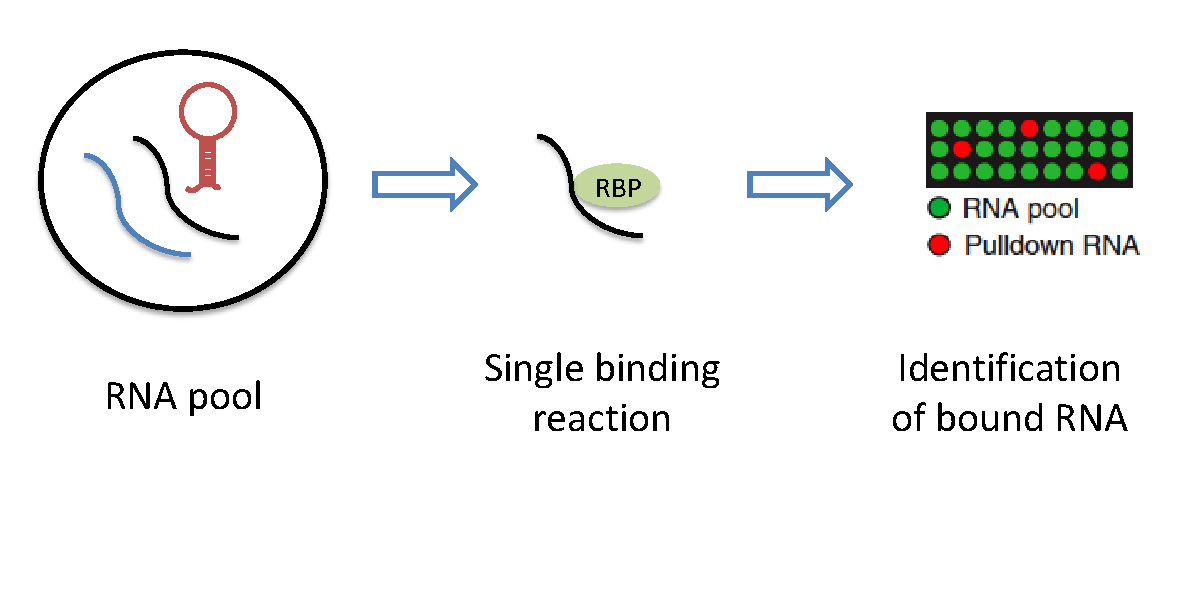
\includegraphics[width=0.6\textwidth,clip]{ch2_background/figures/RNAcompete.pdf}
\caption[Steps in RNAcompete method]{Steps of RNAcompete methods are simplified in this figure (Adopted from RNAcompete \cite{rnacompete_09})}
\label{RNAcompete}
\end{figure}
%\shorthandon{=}


\subsection{In vivo methods}

RNA immunoprecipitation (RIP) is a powerful high-throughput method which detects the association of an individual RBP with specific RNA. This method purifies RBP-mRNA complexes from cellular extracts and identifies protein-bound mRNAs using either a microarray (RIP-chip) or high-throughput sequencing (RIP-seq) \cite{keene_06, zhao_10}. The absence of cross-linking step in this method may lead to dissociation of RBPs from their targets \cite{mili_2004}.

Cross-linking and immunoprecipitation (CLIP or HITS-CLIP) method aims to eliminate the dissociation of RBPs mentioned in the previous method. Figure \ref{PARCLIP_HITSCLIP} shows the steps in PARCLIP and HITS-CLIP methods. This approach utilizes an ultraviolet light (UV) cross-linking step before immunoprecipitation. This enables a more stringent washing procedure to reduce contaminants and eliminate interactions that occur after cell lysis \cite{ule_05}. PARCLIP is a modified version of CLIP technique which uses photoactivatable ribonucleoside-enhanced cross-linking and immunoprecipitation. In this method, cross-linked sites are enriched with a thymidine to cytidine transition \cite{hafner_10}. This method identifies RBP binding sites by scoring T to C transitions in sequenced cDNA. T-C mutations are useful in identification of binding sites in high resolution. CLIP experiments identify the binding sites of a single RBP at a time while a recently proposed method called gPARCLIP (global PARCLIP) identifies the binding sites of all the RBPs that exist in the cell \cite{baltz_12}. However, this method is unable to detect and identify the particular RBPs that bind to a site.

%\shorthandoff{=}
\begin{figure}[H]
   \centering
   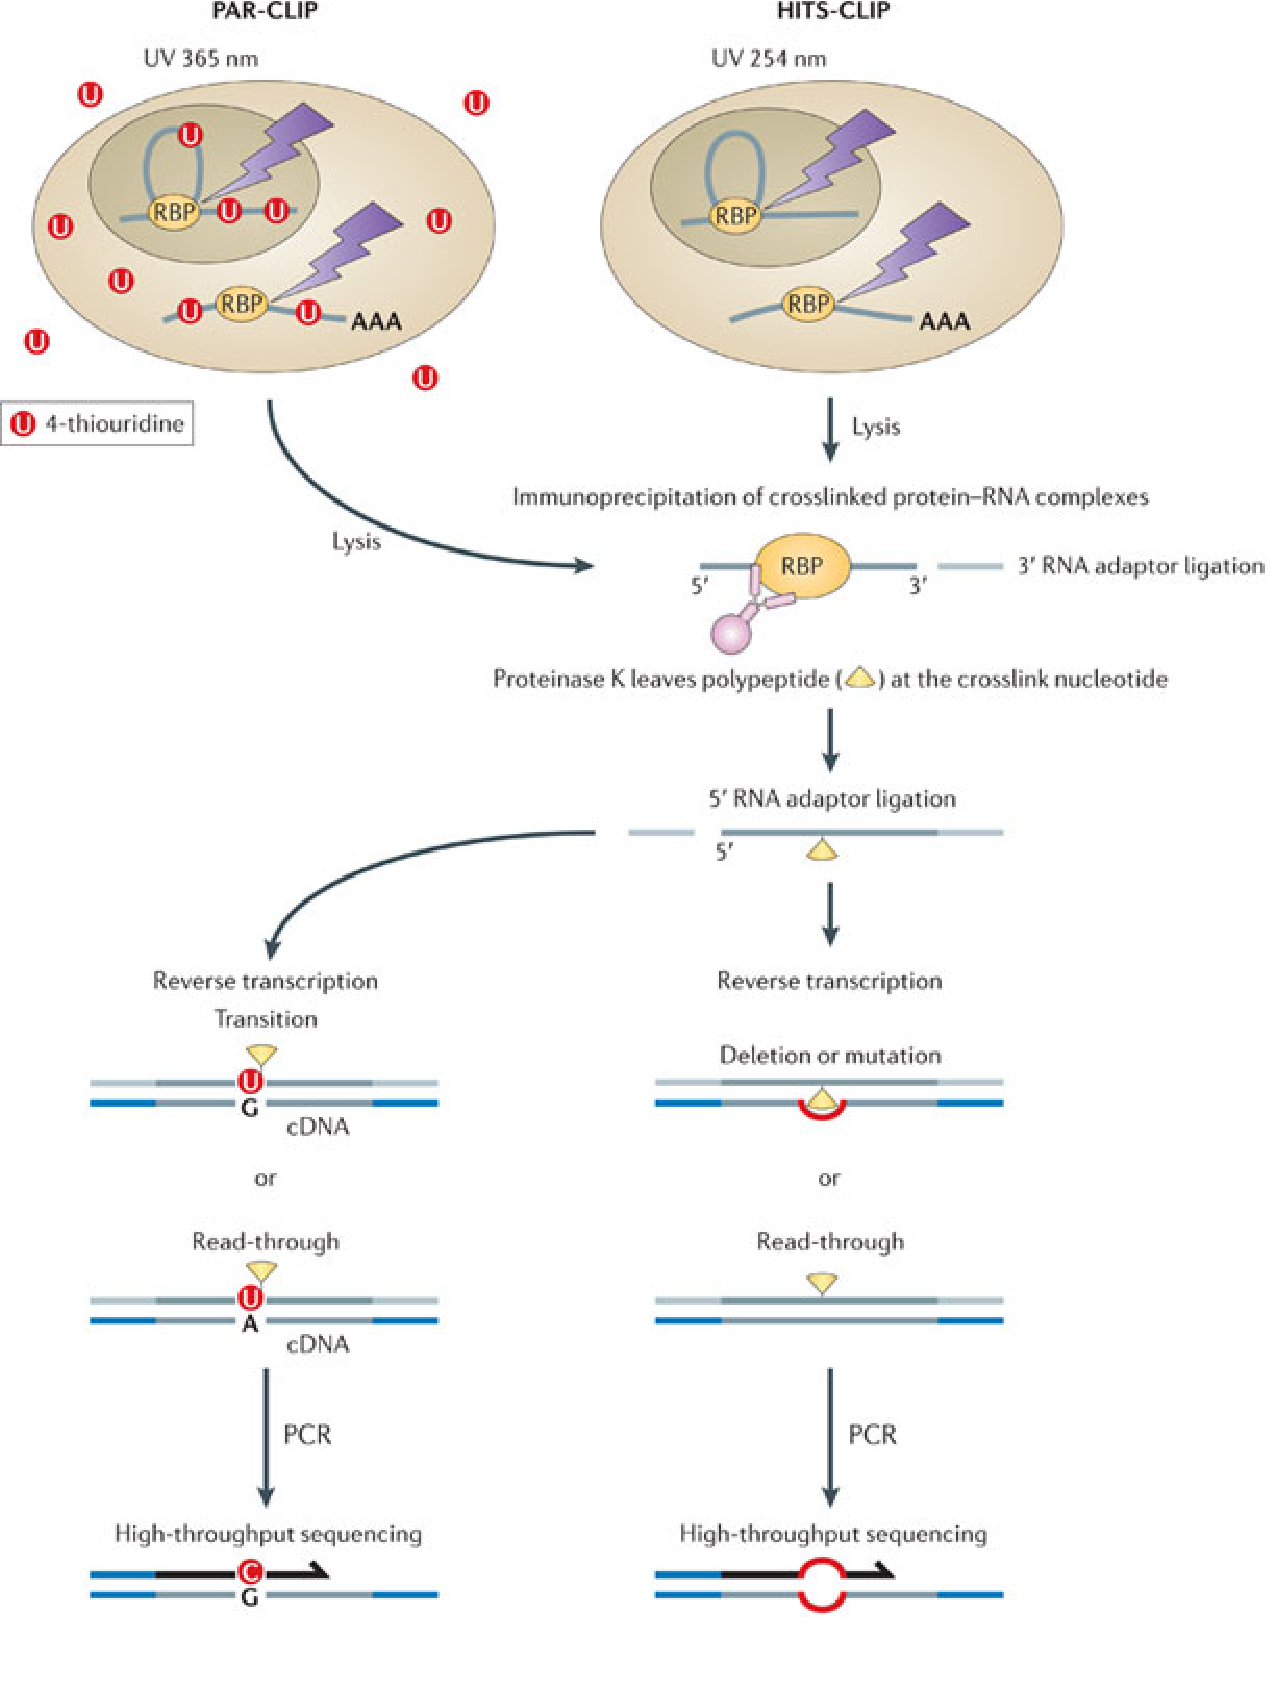
\includegraphics[width=0.5\textwidth,clip]{ch2_background/figures/parclip_hitsclip.pdf}

\caption[Various steps in PARCLIP and HITS-CLIP methods]{Various steps in PARCLIP and HITS-CLIP methods (Figure and description adopted from König et al. \cite{konig_2012})}
\label{PARCLIP_HITSCLIP}
\end{figure}
%\shorthandon{=}

\subsection{In silico methods} 

DNA motif finding tools such as MEME \cite{bailey_06} and HOMER \cite{heinz_2010} are commonly used to identify the binding motifs from a set of RNA sequences that are known to be bound by the RBP. Recently, several methods have been developed to specifically infer RNA motifs that include both sequence and structure features \cite{kazan_10, hiller_06, maticzka_14}. However, all of these methods require a set of bound RNA sequences so that they are based on the results of experimental methods.

De novo prediction of RBP-RNA interactions have been also studied. Pancaldi et. al. \cite{pancaldi_2012}, used more than 100 features such as 3’UTR characteristics, di-nucleotide content, RBP properties, RNA secondary structure statistics to predict the target mRNAs of RBPs in yeast. Muppirala et. al. \cite{muppirala_2011} developed a method called RPIseq that uses the 4-mer composition of the RNA sequence and the 3-mer composition of the RBP sequence to train a statistical model. They try both Support Vector Machine (SVM) and Random Forest (RF) methods to predict whether the RNA-RBP pair will interact or not. These methods have not been tested on a large dataset that contains human RBPs. 


\section{MicroRNAs}

MiRNAs are small (~22 nt long) non-coding RNAs that function in various biological pathways. They regulate gene expression by binding to target mRNAs containing complementary sequences. Recent studies show that over half of the human transcripts are subject to miRNA regulation through degradation or translation inhibition \cite{bartel_2009}. Studies have proved the effect of miRNAs on various cancer types, such as breast, lung, and prostate cancer. They are also implicated in some neurological disorders including schizophrenia and Alzheimer's diseases.

The first miRNA, lin-4, was discovered in \textit{C.elegans} \cite{lee_1993}. The identification of initial miRNAs led to extensive researches which resulted in the rapid discovery of many miRNAs. Currently, there are hundreds of miRNAs in the human genome.

MiRNAs bind to their target sites in 3'UTR of target mRNAs by either complete or partial complementary base pairing. The base pairing usually happens in the 5'-end of the miRNAs. This region is positioned at 2-7 nt of miRNAs and named as the 'seed region'. Complete complementary base pairing in this region is sufficient to downregulate the target mRNA. On the other hand, partial complementary in this region is compensated with additional base pairing in the 3'-end of the miRNAs. Similar to RBP-mRNA interactions, the interactions between miRNAs and mRNAs can be seen as a many-to-many relationship. A miRNA can bind to hundreds of mRNAs and an mRNA can contain target sites of several miRNAs. In the following section, we will briefly introduce the methods to identify miRNA targets.


\subsection{Methods for identification of miRNA binding sites}

Techniques such as qRT-PCR, luciferase reporter assays and western blot can be used to confirm an individual miRNA:mRNA interaction. qRT-PCR and western blot can be used to measure the downstream mRNA and protein expression changes upon the change of miRNA expression. However, these methods cannot distinguish between direct and indirect targets of miRNAs. Reporter assays, on the other hand, can prove a direct link by testing the effect of mutations in miRNA target sites. However, they are labor intensive. 

The methods described above can only be used to identify a small number of targets of the miRNA of interest. To identify the genome-wide targets of an miRNA, high throughput approaches have been also developed. One such approach is to measure the changes of gene expression upon miRNA transfection or inhibition. Microarray or RNA-seq techniques can be used to measure gene expression. One disadvantage of miRNA transfection method is that the miRNA of interest is expressed in higher than natural quantity. This can potentially saturate RISC complexes and affect the function of other endogenous miRNAs. MiRNA inhibition approach is also challenging because the antisense oligonucleotides that are used to inhibit the miRNA may not be specific enough to distinguish between the members of the same miRNA family. These methods still give a good overview of miRNA targets. 

Biochemical approaches to find miRNA targets involve the immunoprecipitation of the RISC component using an antibody against the Argonaute protein \cite{karginov_2007}. Precipitates are then analyzed either by microarray or sequencing to identify the targets. Similar to the identification of RBP sites, cross-linking by ultraviolet radiation technique can also be used here to identify miRNA sites. For instance, PARCLIP has been applied in HEK293 cells \cite{hafner_10}.

The approaches described so far analyze the effects of miRNAs on mRNAs. Measuring the change in protein expression is also important. Stable isotope labelling with amino acids in cell culture (SILAC) is one such method to measure protein abundance using mass spectrometry of samples labelled with different isotopes.


%Genetic methods identify miRNA binding sites through phenotypic suppression tests. The idea behind this approach is to find genes where mutations in miRNA sites rescue the loss of function phenotype of the miRNA. For example, a mutation in lin-41 rescued the bursting vulva phenotype of lethal 7 (let-7) mutant in \textit{C.elegans} \cite{reinhart_2000}. As such, this study shows that lin-4 is a target of let-7. Targets identified by this approach are physiologically relevant; however, the experimental protocol is laborious. As such, they can identify only a few targets of a miRNA. Also, it is not possible to distinguish between direct and indirect miRNA sites with these methods.

%Another approach to identify miRNA binding sites is to use biochemical methods. Initial methods of this kind aimed to isolate the sequence associated with miRNAs using Immunoprecipitation (IP) followed up by microarray or next generation sequencing (NGS) to identify miRNA target sites. Later, researchers took advantage of CLIP methods such as HITS-CLIP and PARCLIP to identify miRNA binding sites. MiRNAs are bound by Argonaute proteins (AGO1-4). Hafner et al. identified miRNA binding sites using PAR-CLIP approach by detecting AGO protein sites . We have discussed these identification methods in the RBPs section. 

MiRNA targets that have been identified by experimental methods are stored in databases. MirTarbase is one such database that contains more than fifty thousand experimentally validated miRNA-target interactions which are compiled by data-mining existing literature \cite{mirtarbase}. Interactions can be validated by several techniques such as reporter assay, western blot, northern blot, qRT-PCR, microarray, pSILAC and NGS based techniques. 

MiRNA targets have been initially determined by time-consuming low-throughput experiments. In the absence of high-throughput experiments, computational methods have been developed to predict miRNA targets. TargetScan is one of the most widely used method which considers complementarity to seed region and conservation information to predict miRNA target sites \cite{targetscan_05}. TargetScanS extends TargetScan by also taking into account other metrics such as local A-U content, target site position, target abundance, seed pairing stability, 3’ contribution. PicTar is another computational method that first assigns a probability to potential target sites based on base-pairing to seed region and conservation. These probabilities are then used in a hidden Markov model (HMM) to calculate the probability of generating the 3’UTR region by states that correspond to miRNA binding sites or background \cite{pictar_05}. GenMiR integrates matched mRNA-miRNA expression data into a Bayesian probabilistic model to predict miRNA targets \cite{genmir_2007} The likelihood of this model is calculated by a linear model that models the change in the expression level of potential targets to the expression of targeting miRNAs. GenMiR starts from an initial network of miRNA-mRNA targets that are predicted by TargetScan.

The regulatory effect of miRNAs depends on several factors. First, the location and secondary structure of binding sites may enhance the chance of miRNAs to bind to their targets. Studies show that AU-rich regions and unstructured areas such as 3'UTRs are more likely to be miRNA binding sites. Second, the number of miRNA binding sites plays a crucial role in the regulation of mRNAs. The more binding sites a transcript contains, the higher probability that it will be extensively regulated. Besides, miRNAs may involve in collaboration and competition interactions with RBPs. So far, most of the studies investigated the effect of one of these factors independently. However, recent studies show that miRNAs and RBPs are involved in complex gene regulation mechanisms. In the following sections, we first introduce RNA secondary structure which is important in recognition of binding sites of miRNAs and RBPs. Next, we briefly review previous work on the cooperative and competitive interactions between miRNAs and RBPs.

\clearpage
\section{RNA secondary structure}

A single-stranded RNA molecule can fold back onto itself forming a secondary structure. The most common base-pairs are the Watson-Crick base pairs A-T and G-C and the G-U wobble pair.

%\shorthandoff{=}
\begin{figure}[H]
   \centering
   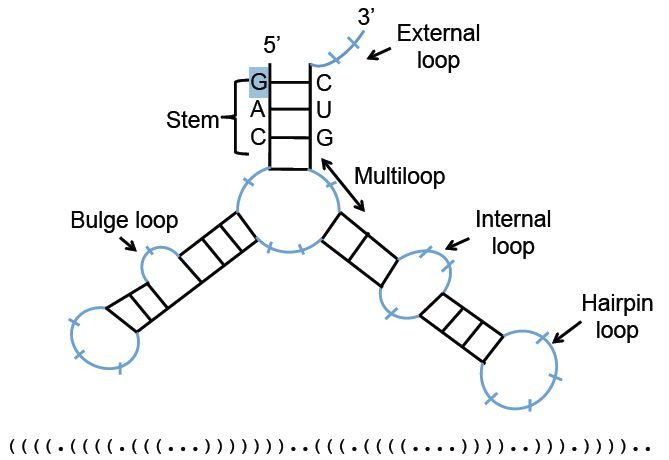
\includegraphics[width=0.8\textwidth,clip]{ch2_background/figures/secondary_structure}

\caption[Example of RNA Secondary Structure]{An RNA secondary structure example. One or more consecutive base pairs form a stem. Unpaired bases form various kinds of loops (shown in blue).}
\label{secondary_structure}
\end{figure}
%\shorthandon{=}

We can represent RNA secondary structure formally by assigning an index to each base in the RNA sequence. For example, we can start from the left end of the RNA sequence (5’end) and index each base by proceeding to the right end (3’end). If we assume that the indexing starts from 1 and the length of the sequence is N, a secondary structure S can be defined as a set of pairs i-j, 1 <= i < j <= N where each base is only paired with at most one other base. A stack of base pairs is called a stem.

Figure \ref{secondary_structure} shows an example secondary structure. Unpaired regions that are enclosed by one or more base pairs are called loops. They are several kinds of loops according to the number of closing base pairs. A hairpin loop is a circular end to a hairpin stem and it happens when there is a single closing base pair. A bulge or internal loop happens when there are two closing base pairs. Multi-loops have more than two closing base pairs. Finally, an external loop happens when the unpaired bases are at the end of the sequence. The same structure is shown with a dot-parenthesis notation on the bottom of the figure. In this notation, a matching pair of parentheses indicates a base pair and a dot denotes an unpaired base. 

There are several experimental techniques to determine the secondary structure of a RNA. However, these methods are difficult and time-consuming. Besides, experimental methods are unable to characterize the structures of many RNAs because of their conformational flexibility and large size. There are also methods in which scientists use chemical probing to increase the accuracy and the throughput of probing experiments \cite{kertesz_2010, FragSeq_2010, SHAPEseq_2011}. The basic idea behind this method is to use chemical reagent which leaves and imprint on the RNA molecule. These imprints can then be used to distinguish paired and unpaired nucleotides. These experiments, however, only report partial information of the structure.

There are three general categories for RNA secondary structure prediction algorithms: (i) comparative methods that infer the secondary structure common to aligned sequence across conserved species; (ii) thermodynamic methods that predict the structure with the minimum free energy (MFE); and (iii) probabilistic models that use parameters learned from known structures to predict unknown structures.

The comparative approach is most accurate when several aligned homologous RNA sequences are available \cite{gardner_04}. The disadvantage of this approach is that it is limited to datasets where the sequences are similar enough to get a reliable alignment. Therefore, these methods are not suitable to determine the secondary structure of all \textit{in vitro} and \textit{in vivo} data sets for any organism.

The second approach for discovering secondary structure is to use a set of thermodynamic parameters that predict the folding free energy of a given structure and a dynamic programming algorithm to find the structure with minimum free energy \cite{mathews_1999, mathews_06}. The idea behind this approach is that RNAs fold to the structure with the minimum free energy. One of the disadvantages of this approach is that an RNA molecule can fold into multiple structures during its lifetime. Therefore, the predicted MFE structure may not be the real, functional structure. One possible solution to address this issue is to consider the distribution of possible structures.

RNAfold is a method of this kind which computes probabilities for every possible base pair from the partition function. RNAplfold is a variant of RNAfold which uses local folding instead of global folding. This method considers base pairs within a certain span and calculates average base pair probabilities by averaging over all windows of a certain length that contain the pair. Studies show that this method performs more accurate than the classic global folding algorithms \cite{lange_12}. This algorithm uses little amount of memory and CPU time to run and therefore it is practical to scan large scale of the genome for short RNA structure.

SFOLD generates a statistical sample of RNA secondary structures from the Boltzmann ensemble of RNA secondary structures \cite{sfold}. Individual structures that are sampled by SFOLD can be used to calculate various probabilities such as probability of a region to form a stem with another region. 

Probabilistic models use parameters estimated from known RNA structures to predict secondary structure. There is also a method, called SimFold, which combines thermodynamic parameters and probabilistically estimated parameters \cite{andronescu_10}. These methods are becoming more powerful due to the increasing availability of known RNA structures.


\section{Competition and collaboration between RBPs and miRNAs}

Recent studies show that the RBPs and miRNAs, two major classes of post-transcriptional regulators, do not act independently. Instead, they are involved in competitive or cooperative interactions with each other. As such, the net outcome of target mRNA expression relies heavily on the interplay between these two classes of trans-acting factors. Here, we review some examples of these interactions.

\subsection{Collaboration between RBPs and miRNAs}

Jing et al. investigated the collaborative interaction between TTP and miR-16 which leads to the degradation of their target COX-2 mRNA \cite{jing_2005}. Both of these factors target the same AU-rich element (ARE) and as such, they are involved in direct interaction. In this study, they discovered that TTP interacts with miR-16 through association with AGO protein which assists miR-16 to bind to its target site. This process enables miR-16-mediated repression of COX-2 mRNA.

Interactions of HuR with miRNAs have been extensively studied as well. Kim et al. \cite{kim_2009} show that HuR and let-7 miRNA have to act together to repress translation of their target mRNA c-MYC. These two trans-acting factors repress c-MYC through an interdependent mechanism. In this study, they mutated the let-7 interaction sites and compared it with the wildtype case. They observed that segments with mutated let-7 sites did not respond to HuR silencing enhancement. On the other hand, they show that HuR is necessary for let-7 interaction with c-MYC mRNA. However, the underlying mechanism is still unclear. They suggest that HuR binding might change the local RNA structure, unmasking the let-7 recognition site.

Another interesting example is the cooperative interaction between the RBP PUM1 and the miRNAs miR-221/222 on the 3’UTR of the tumor suppressor gene p27 \cite{kedde_10}. Figure \ref{pum_miR-221} illustrates the binding sites of PUM1 and miR-221/222 on two sides of a same stem-loop. Binding of PUM1 protein alters the secondary structure and allows miR-221/222 to bind to the other side of the stem-loop. The cooperative interplay between these two factors leads to faster downregulation of p27.

%\shorthandoff{=}
\begin{figure}[H]
   \centering
   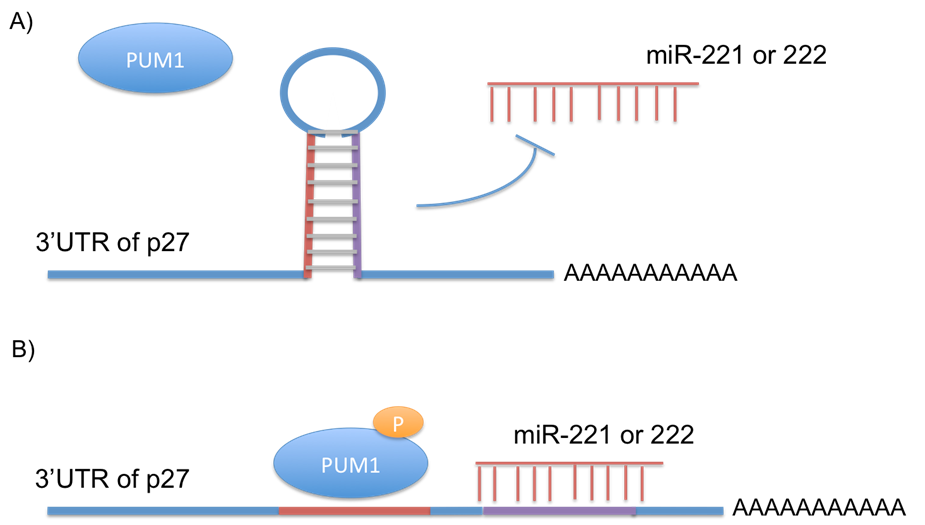
\includegraphics[width=0.8\textwidth,clip]{ch2_background/figures/pum_miR221.pdf}

\caption[Cooperative interaction between PUM1 and miR-221/222]{Cooperative interaction between PUM1 and miR-221/222.}
\label{pum_miR-221}
\end{figure}
%\shorthandon{=}

Figure \ref{pum_miR-221} shows the collaboration between PUM1 and miR-221/222. Without the PUM1, miR-221/222 is unable to bind to its target on p27 mRNA. Binding of PUM1 to its target in one side of the stem loop alters the secondary structure and makes it available for miR-221/222 to bind to the other side of the same loop. Their cooperation leads to faster degradation of their target mRNA.

\subsection{Competition between RBPs and miRNAs}

HuR has been shown to enhance the overall gene expression of both CAT-1 and COX-2 by protecting them from inhibitory action of miR-122 and miR-16, respectively \cite{bhattacharyya_2006, young_2012}. In the first case (CAT-1), HuR gets dephosphorylated and translocated from nucleus to the cytosol, where it binds to target ARE sequences on CAT-1 mRNAs and increases stability. This phenomenon leads to dissociation of miR-122 containing RISCs from CAT-1 mRNAs. Indeed, researchers also show that HuR is also able to displace the already bound RISCs. In the second case, HuR and miR-16 target the same ARE on COX-2 mRNA. In colorectal cancer cells, HuR gets overexpressed and localizes to the cytoplasm \cite{young_2012}. Under these conditions miR-16 is unable to promote mRNA decay. HuR is shown to directly associate with miR-16; however how HuR antagonizes miR-16 is still unclear. 

Another example of competition between RBPs and miRNAs is the translocation of the RBP HNRNPL under hypoxia conditions to compete with several miRNAs, including miR-297 or miR-299, on VEGFA 3’UTR through a CA-rich element. Binding of HNRNPL relieves VEGFA mRNA from miRNA-mediated repression.

The examples mentioned above provide a summary of known interactions between RBPs and miRNAs. Given the number of existing RBPs and miRNAs, these interactions constitute only a minority of the existing interactions between RBPs and miRNAs. These studies have focused on a single RBP or a single miRNA as laborious experiments are needed to confirm the interactions. Computational studies that scan for interactions between all RBPs and miRNAs can guide experimental studies. In the following section, we introduce two studies which aim to investigate combined effect of multiple factors in PTR.

\subsection{High-throughput techniques considering several factors}

Mukharjee et al. analyzed the combinatorial regulation by HuR and miRNAs \cite{mukharjee_11}. They investigated the condition in which binding sites of HuR and miRNAs overlap with each other. Their findings show that the existence of overlapping HuR sites relieves miRNA-mediated repression. However, the existence of overlapping miRNA sites has no effect in regulation mediated by HuR protein. This indicates that HuR is likely to compete with miRNAs for binding sites and stabilizes the targeted mRNAs.

In another study, researchers analyzed the effect of possible interactions between a few RBPs and miRNAs \cite{jiang_13}. They investigated the positional relationship of motif occurrences and observed that a particular RBP and an miRNA may interact with each other when there is a specific distance between their binding sites. For example, they showed that specific miRNAs tend to bind near PUM binding sites. These miRNAs have recognition seeds that are reverse complementary to the PUM recognition motifs. They show that PUM increases the accessibility of the sites for its interacting miRNAs which results in cooperation to promote mRNA decay. MiR-101, miR-300, miR-144, miR-221/222 are some examples of miRNAs that are predicted to interact with PUM. This is in accordance with the previous paper we described above, in which miR-221/22 pairs up with the PUM recognition sequence and cooperate with this protein to repress their target mRNA. 

Most of the previous studies have ignored the effect of RNA secondary structure whereas it is important in recognition of binding sites of RBPs and miRNAs. It is also beneficial to take advantage of existing knowledge on RBP binding, miRNA binding and mRNA stability by compiling CLIP datasets, experimental miRNA targets and genome-wide datasets of knockdown or transfection experiments. To the best of our knowledge, a comprehensive study of cooperative and competitive interactions between pairs of factors (i.e., all RBPs and miRNAs) is still lacking. In this thesis, we aim to investigate RBPs and miRNAs cooperative and competitive interaction comprehensively. First, we map the binding sites of RBPs and miRNAs on human 3’UTRs. Next, we utilize this comprehensive collection of sites to investigate interplay between each pair of factors and to predict half-life and mRNA abundance by considering effects of both RBPs and miRNAs.


% CHAPTER 3
\chapter{MATERIALS AND METHODS}
\label{chp:chapter3}

\section{Mapping RBP binding sites}
To map the binding sites of RBPs, we downloaded 103 position frequency matrices (PFMs) that correspond to 85 human RBPs from the RNAcompete paper \cite{rnacompete_13}. These PFMs (which are of length seven or eight) are generated from the alignment of top 10 7-mers determined using all data (i.e. both setA and setB of RNAcompete pool). Rather than using these top 10 7-mers directly, we generated the top 10 n-mers from these PFMs. In this way, we also represented motifs that are longer than seven. In addition to RNAcompete motifs, we downloaded the motifs (consensus motifs and the top 10 n-mer when a PFM is available) for the following well-known RBPs from RBPDB database \cite{rbpdb_11}: HNRNPAB, PUM1, PUM2, ELAVL2, KHSRP, ZFP36, AUF1 and CUGBP. 

We downloaded human 3'UTRs from UCSC Genome Browser (on February 16th, 2014) and determined the genome-wide binding sites of each RBP by finding matches to its top 10 n-mers or consensus motifs on human 3'UTR sequences. We downloaded CLIP-seq and PARCLIP data for a list of RBPs (HuR, FMR1, FUS, FXR1, FXR2, HNRNPA1, HNRNPA2B1, HNRNPC, IGF2BP1-3, LIN28, PUM2, QKI, SRSF1, TDP-43, TIA1, TIAL1) from doRINA database \cite{dorina_11}. In addition to these RBP specific CLIP datasets, we downloaded gPARCLIP-determined peaks \cite{baltz_12}. gPARCLIP dataset contains genome-wide protein-occupied regions bound by any RBP in HEK293T cells. However, the identity of a particular RBP that binds to a region is unknown. 

We first intersected the peaks identified with CLIP or gPARCLIP  with human 3'UTRs. To correct for the background binding bias in CLIP-based techniques as identified by Friedersdorf et al. \cite{friedersdorf_14}, we excluded parts of peaks that overlap with regions that correspond to background binding. In summary, for each putative RBP site we keep track of the following information: (i) the start and end position; (ii) a flag showing whether the site is located in a CLIP- or gPARCLIP-determined peak; and (iii) conservation score calculated as the average PhastCons score \cite{siepel_05} (phastCons100way track downloaded from UCSC Genome Browser) across the motif (Figure \ref{overview}).

\clearpage

\section{Mapping miRNA binding sites}
To determine miRNA binding sites, we downloaded the target sites predicted by TargetScan and PicTar methods \cite{targetscan_05, pictar_05}. We downloaded AGO1-4 PARCLIP, AGO2 CLIP-seq and AGO2-MNase PARCLIP datasets from doRINA database, and removed background binding bias as described in the previous section. We also downloaded experimentally verified miRNA targets from miRTarBase database \cite{mirtarbase}. The interactions in miRTarBase database specify only whether a miRNA interacts with an mRNA without providing the exact position of the target site on the mRNA. Therefore, we assumed that a target miRNA site on an mRNA is supported by miRTarBase if that miRNA-mRNA interaction exists in the database. For each putative miRNA binding site, we keep track of its start and end position, a flag showing whether the site is supported by TargetScan, PicTar or both, a flag showing whether it is supported by miRTarBase and a flag whether the site is located in CLIP- or PARCLIP-determined peaks (Figure \ref{overview}).

\section{Compilation of datasets related to post-transcriptional regulation}

The following datasets were downloaded from the supplementary material of the corresponding papers:
\begin{itemize}
\item \textbf{Knockdown datasets:} Log fold changes (LFCs) of transcript abundance upon HuR knockdown in  HEK293 and HeLa cells from \cite{mukharjee_11} and \cite{lebedeva_11}, respectively. 
\item \textbf{Zhao dataset:} The effect of human 3'UTR segments (160-nts long) to mRNA stability and steady-state mRNA abundance in BEAS-2B human bronchial epithelial cells \cite{zhao_14}.
\item \textbf{Schueler dataset:} mRNA half-lives measured in HEK293 and MCF7 cells \cite{schueler_14}. Average of the two replicate measurements is used. 
\end{itemize}

\clearpage
%\shorthandoff{=}
\begin{figure}[H]
   \centering
   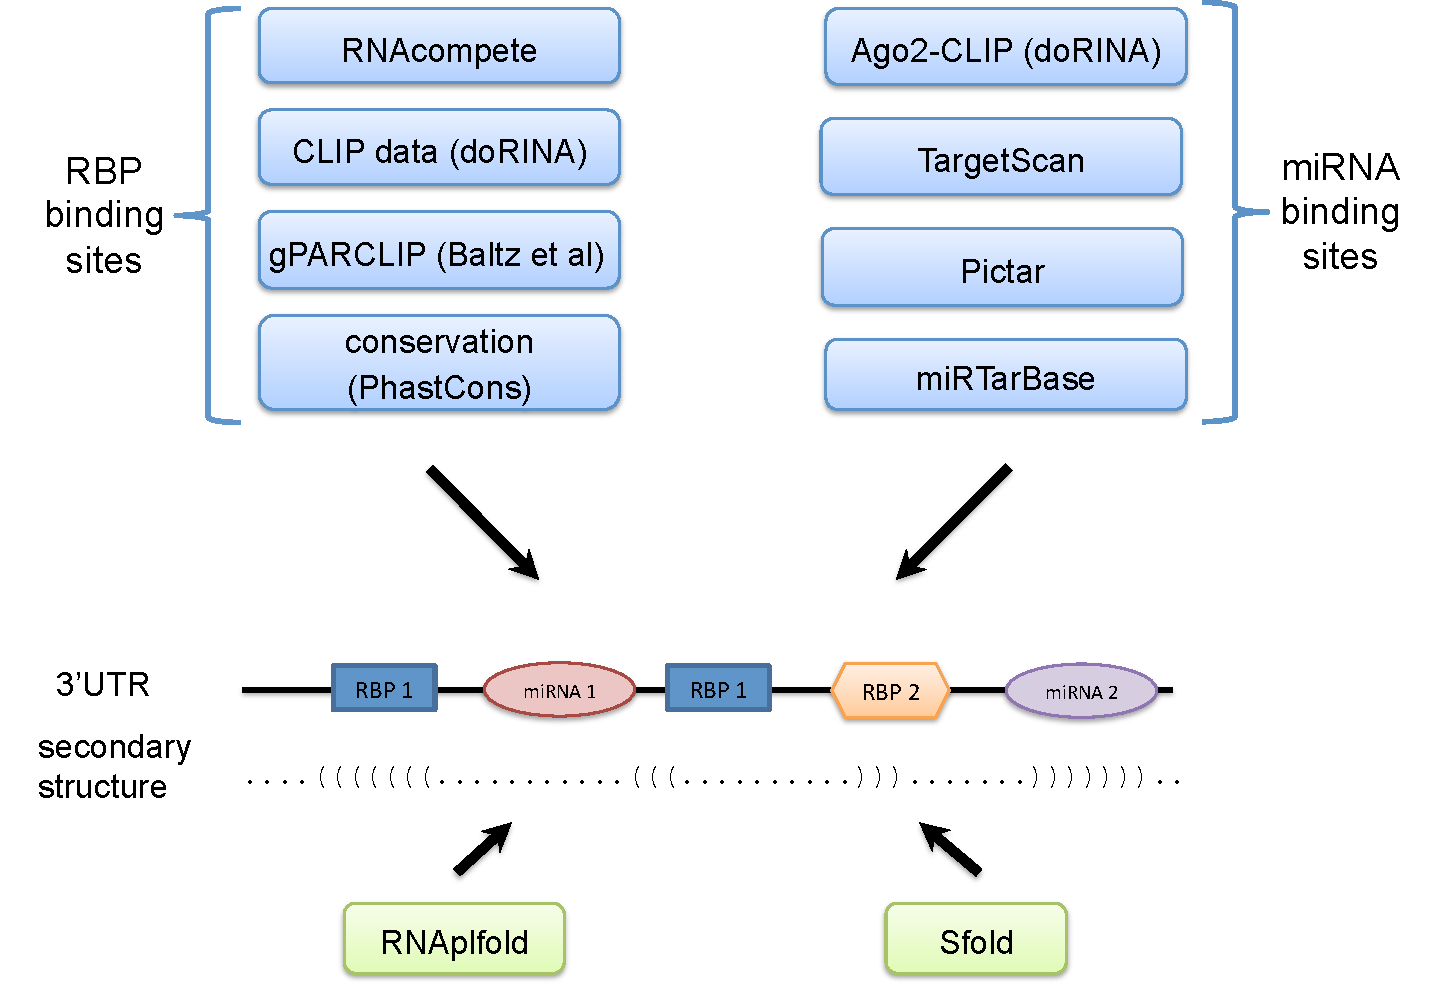
\includegraphics[width=0.7\textwidth]{ch3_materials_methods/figures/Figure1}

\caption[]{Mapping of RBP and miRNA binding sites on human 3'UTRs. RBP binding sites are mapped by leveraging RNAcompete PFMs, CLIP- and PARCLIP-determined peaks and PhastCons conservation scores. miRNA binding sites are mapped by combining TargetScan and PicTar predictions with Ago-CLIP datasets and experimentally-verified interactions in miRTarBase database. Also, the secondary structure of the 3'UTRs are predicted with RNAplfold and Sfold. In particular, accessibility of a site is calculated by RNAplfold, and the probability of a site to form a stem-loop by binding to another site is calculated by Sfold.}
\label{overview}
\end{figure}
%\shorthandon{=}


The set of expressed RBPs and miRNAs vary widely between different cell lines. As such, it is important to consider only those factors that are expressed in the corresponding cell line in the analysis of  the datasets above. We used the following sources to define the set of expressed RBPs and miRNAs in a given cell type:
\begin{itemize}
\item HEK293 cells: 
\begin{itemize}
\item RBPs: quantitative mass spectrometry results  \cite{baltz_12}.
\item miRNAs: top 100 expressed miRNAs identified with small-RNA sequencing \cite{hafner_10}.
\end{itemize}
\item HeLa cells:
\begin{itemize}
\item RBPs: immunohistochemistry results from Human Protein Atlas database \cite{proteinatlas}.
\item miRNAs: top 100 expressed miRNAs identified with small-RNA sequencing \cite{lebedeva_11}.
\end{itemize}
\item MCF7 cells:
\begin{itemize}
\item RBPs: immunohistochemistry results from Human Protein Atlas database.
\item miRNAs: top 100 expressed miRNAs identified with small-RNA sequencing \cite{anbalagan_14}.
\end{itemize}
\item BEAS-2B cells:
\begin{itemize}
\item RBPs: immunohistochemistry results from Human Protein Atlas database.
\item miRNAs:  top 100 expressed miRNAs identified with small-RNA sequencing \cite{zhao_14}.
\end{itemize}
\end{itemize}

For datasets that contain measurements mapped to gene IDs other than human RefSeq transcript IDs, we used the Synergizer tool for ID conversion \cite{synergizer}. 

We also checked the overlap in the set of expressed RBPs across the cell lines. Tables \ref{tbl:expressed_rbps} and \ref{tbl:expressed_mirnas} show the number of expressed RBPs and miRNAs in each cell line along with the percent overlap of expressed RBPs in different cell lines.
\hfill

\begin{table}[H]
\caption[Number of expressed RBPs in each cell line]{The numbers within parenthesis correspond to the total number of RBPs expressed in that cell line. Besides, percent of overlapping expressed RBPs between each pair of cell lines are shown. For example, \%95.65 of expressed RBPs in HEK293 cells are also expressed in HeLa cells. On the other hand, \%80.73 of expressed RBPs in HeLa cells are also expressed in HEK293 cells.}
\begin{tabular*}{\textwidth}{l @{\extracolsep{\fill}} c c c c}
%\rowcolor{LightCyan}
Cell types &  HEK293 (92) & HeLa (109) & BEAS2B (97) & MCF7 (102) \\ [0.5ex]
\hline\hline
HEK293 (92) & \cellcolor{Gray} & \%95.65 & \%90.22 & \%93.48 \\
\hline
HeLa (109) & \%80.73 & \cellcolor{Gray} & \%88.99 & \%93.58 \\
\hline
BEAS2B (97) & \%85.57 & \%100 & \cellcolor{Gray} & \%97.94 \\
\hline
MCF7 (102) & \%84.31 & \%100 & \%93.14 & \cellcolor{Gray} \\ 
\hline
\end{tabular*}
\label{tbl:expressed_rbps}
\end{table}

\begin{table}[H]
\caption[Number of expressed miRNAs in each cell line]{The numbers within parenthesis correspond to the total number of miRNAs expressed in that cell line. Besides, percent of overlapping expressed miRNAs between each pair of cell lines are shown. For example, \%68.29 of expressed miRNAs in HEK293 cells are also expressed in HeLa cells. On the other hand, \%62.92 of expressed miRNAs in HeLa cells are also expressed in HEK293 cells.}
\begin{tabular*}{\textwidth}{l @{\extracolsep{\fill}} c c c c}
%\rowcolor{LightCyan}
Cell types &  HEK293 (82) & HeLa (89) & BEAS2B (78) & MCF7 (100) \\ [0.5ex]
\hline\hline
HEK293 (82) & \cellcolor{Gray} & \%68.29 & \%64.63 & \%50 \\
\hline
HeLa (89) & \%62.92 & \cellcolor{Gray} & \%57.3 & \%52.81 \\
\hline
BEAS2B (78) & \%67.95 & \%65.38 & \cellcolor{Gray} & \%48.72 \\
\hline
MCF7 (100) & \%41 & \%47 & \%38 & \cellcolor{Gray} \\ 
\hline
\end{tabular*}
\label{tbl:expressed_mirnas}
\end{table}

It is clear from tables \ref{tbl:expressed_rbps} and \ref{tbl:expressed_mirnas} that the high percent of RBPs are expressed in all four cell lines. Each pair of cell lines have over \%90 overlapping expressed RBPs between each other. It is not the same in case of miRNAs though. We compared the expressed miRNAs between each cell types and observed that around half of them are shared between each pair of cell lines.

\section{Predicting the RNA secondary structure of binding sites}
\label{sec:structure}
To determine whether binding sites are accessible, we predicted RNA secondary structure of human 3'UTRs with RNAplfold \cite{RNAplfold}. Since the flanking regions can affect secondary structure, we folded the 3'UTRs together with the upstream 200nt-long flanking sequence from coding region. Lange et al. has previously shown that local folding with a window length of 200 and base pair span of 150 gives optimal results compared to using other parameters or global folding \cite{lange_12}. As such, we applied local folding by running RNAplfold with the parameters $\text{-W } 200$ and $\text{-L } 150$ where '-W' specifies the length of the local window and '-L' restricts the maximal base pair span. We used the base pair probabilities output from RNAplfold to determine accessibility. Namely, we calculated the average probability of being in unpaired context across the site and classified the site as accessible if this value is greater than $0.6$ and inaccessible if the value is less than $0.4$. 

As in the example of PUM1-miR-221 (or miR-222) interplay \cite{kedde_10}, factors can act in cooperation by binding to the two sides of the same stem-loop. In this way, one of the factors can allow the other factor to bind its site by changing the secondary structure (i.e., accessibility) of the region. To identify similar potential cooperative interactions, we calculated the number of base pairs that can be formed between each pair of sites by considering reverse complementarity only. We deemed the pairs of sites that have $\geq 5$ base pairs as potential interactors. As one site can be reverse complementary to several other sites, we need to choose the partner site that is most likely to form a stem-loop. To find a quantitative metric for this purpose, we used SFOLD to generate 1000 sample structures from the Boltzmann distribution of all possible structures for each running window of length 200nt. For each pair of binding sites, we considered those windows that both sites are located in, and parsed all the sampled structures of each window to calculate the average number of base pairs formed between the two sites. This value reflects the probability that the two sites will form a stem-loop. 

In order to determine the pairs of sites that could form a stem-loop, we sorted the potential interacting sites (determined by reverse complementarity only) according to SFOLD-calculated probabilities, and filtered out those that have a probability less than 0.1. We started from the top of this list and selected pairs of sites iteratively. We ignored alternative possible interacting sites of an already selected site. For example, let's assume that a particular 3'UTR contains three sites labeled as A, B and C, and each pair of these sites can form a stem-loop with more than  $\geq 5$ base pairs. Let's also assume that the Sfold-calculated probabilities for these pairs are as follows: A-B: 0.3, B-C: 0.6, A-C: 0.4. With our procedure, B-C pair would score the highest and get selected, whereas A-B and A-C pairs would be ignored as B and C are already considered. 

\section{Testing for significance}
We used two-tailed Mann-Whitney U test (also called Wilcoxon rank-sum test) to compare various properties (e.g. log fold change, stability) of sets of transcripts (see Results section), and we used Wilcoxon signed-rank test to compare the area under the ROC curve (AUROC) values of different logistic regression models.

\section{Determining RBP and miRNA binding sites co-occurrence}

To determine the co-occurrence between binding sites of a factor with all other factors (i.e., all RBPs and miRNAs), we followed a similar method discussed in Jiang et al. \cite{jiang_13}. At first step, for each site of a factor, we calculated the number of neighboring sites of other factors in each 50-nt-window 500-nt on either side of the site. Next, we calculated the impractical P-value by comparing this count to the distribution of counts obtained when factor identities are shuffled 10000 times (keeping the site positions fixed). We repeated this permutation test three times, using different shuffling types: (i) shuffling the factor identities of sites that are located on the same chromosome; (ii) classifying the sites into three groups based on AU-content (i.e., $<3$,  $\geq 3$ and $< 6$, $\geq 6$ ) and shuffling the factor identities of the sites in the same group; (iii) classifying the sites into 10 groups according to their relative position within the 3'UTRs and shuffling the factor identities of the sites in the same group (see \cite{jiang_13} for more details). In order to correct the P-values for multiple testing, we converted them into q-values which are a measure of significance in terms of false discovery rate rather than the false positive rate \cite{qvalue}.

\section{Predicting stability and expression using logistic regression}

We used a logistic regression model in order to consider the effect of multiple factors on stability and gene expression levels. We used the following datasets: (i) Effect of 3'UTR segments to mRNA half-lives and steady-state mRNA abundance in BEAS-2B immortalized human bronchial epithelial cells (Zhao dataset, \cite{zhao_14}) (ii)  mRNA half-lives  in HEK293 and MCF7 cells (Schueler dataset, \cite{schueler_14}). We sorted 3'UTR segments or transcripts based on half-lives or abundance and filtered out those that do not have any miRNA or RBP site. We classified the top 500 transcripts as one class (stable or highly expressed) and the bottom 500 transcripts as the other class (unstable or lowly expressed). We labeled the sequences in the first class with 1 and the second class with 0. Our features consist of counts of dinucleotides and counts of sites of factors where factors are grouped as \textit{miRNAs}, \textit{activators}, and \textit{repressors}. We defined the \textit{activators} and \textit{repressors} as sets of RBPs that are known to increase or decrease stability in literature, respectively. Namely, \textit{activators} group consists of the RBPs  HNRNPL, PABPC1, PABPC3, PABPC4, PABPC5, PABPN1, RBFOX1, TIA1, HuR, IGF2BP2 and IGF2BP3; and \textit{repressors} group consists of the RBPs CUGBP1, MBNL1, HNRNPC, KHSRP, ZFP36, AUF1, PUM1 and PUM2. We used the glmnet package to fit a logistic regression model with L2 regularization. We repeated 10-fold cross validation (CV) 10 times and plotted the interpolated area under ROC curve (AU-ROC) of 100 curves.

To run logistic regression with L2 regularization, we used the glmnet package \cite{glmnet} with alpha parameter set to 0. Within each cross-validation run, we ran the \textit{cv.glmnet} function to determine the optimal lambda (i.e. regularization constant) value. 
% CHAPTER 4
\chapter{RESULTS AND DISCUSSION}
\label{chp:chapter4}

In the first step, we assess how accessibility and conservation differ between experimentally supported sites and other sites that are only computationally predicted. Initially, we perform this analysis considering CLIP-supported sites of PUM2, HuR, IGF2BP1-3 and QKI. Next, we inquire the effect of competition between binding sites of HuR and binding sites of other factors in term of mRNA abundance. Also we compare HuR CLIP-supported sites with other sites which are not experimentally validated. In order to investigate the possible interactions between RBPs and miRNAs, we analyze the co-occurrence of binding sites of all factors with each other. Furthermore, we focus on PUM1(2) and analyze the effect of number of PUM1(2) binding sites on the stability of its target mRNAs. Besides, we investigate the effect of situation in which PUM1(2) binding sites tend to localize close to each other on the expression of transcripts. We show that number of PUM1(2) sites along with their distance from each other may play crucial role in stability of their target mRNAs. Finally, we use logistic regression with features compiled from the counts of sites of factors and dinucleotides to accurately predict the stability and steady-state abundance of mRNAs.

\section{Overview of our compendium of RBP and miRNA binding sites}

As discussed earlier in the materials and methods section, we mapped RBP and miRNA binding sites on human 3'UTR. Figure \ref{rbp_stat} shows the venn diagram of the distribution of RBP binding sites supported by CLIP and/or gPARCLIP. All of the RBP binding sites comes from RNAcompete method, which about \%67 of them are supported by experimental methods. Among experimentally validated binding sites, the majority of them are from gPARCLIP method. Furthermore, figure \ref{mirna_stat} shows the venn diagram of the overlap between miRNA binding sites predicted by TargetScan and/or PicTar methods. Also it shows the intersection between number of computationally predicted miRNA binding sites and experimentally validated miRNA targets from mirTarBase and AGO2CLIP methods. As discussed earlier, we used both TargetScan and PicTar computational methods to predict miRNA binding sites. Almost \%93 of miRNA binding sites come from TargetScan method and the rest of them are supported by PicTar. There are 2228 miRNA binding sites which are supported by both of these methods.

%\shorthandoff{=}
\begin{figure}[H]
	\centering
   	\subfloat[]{
   	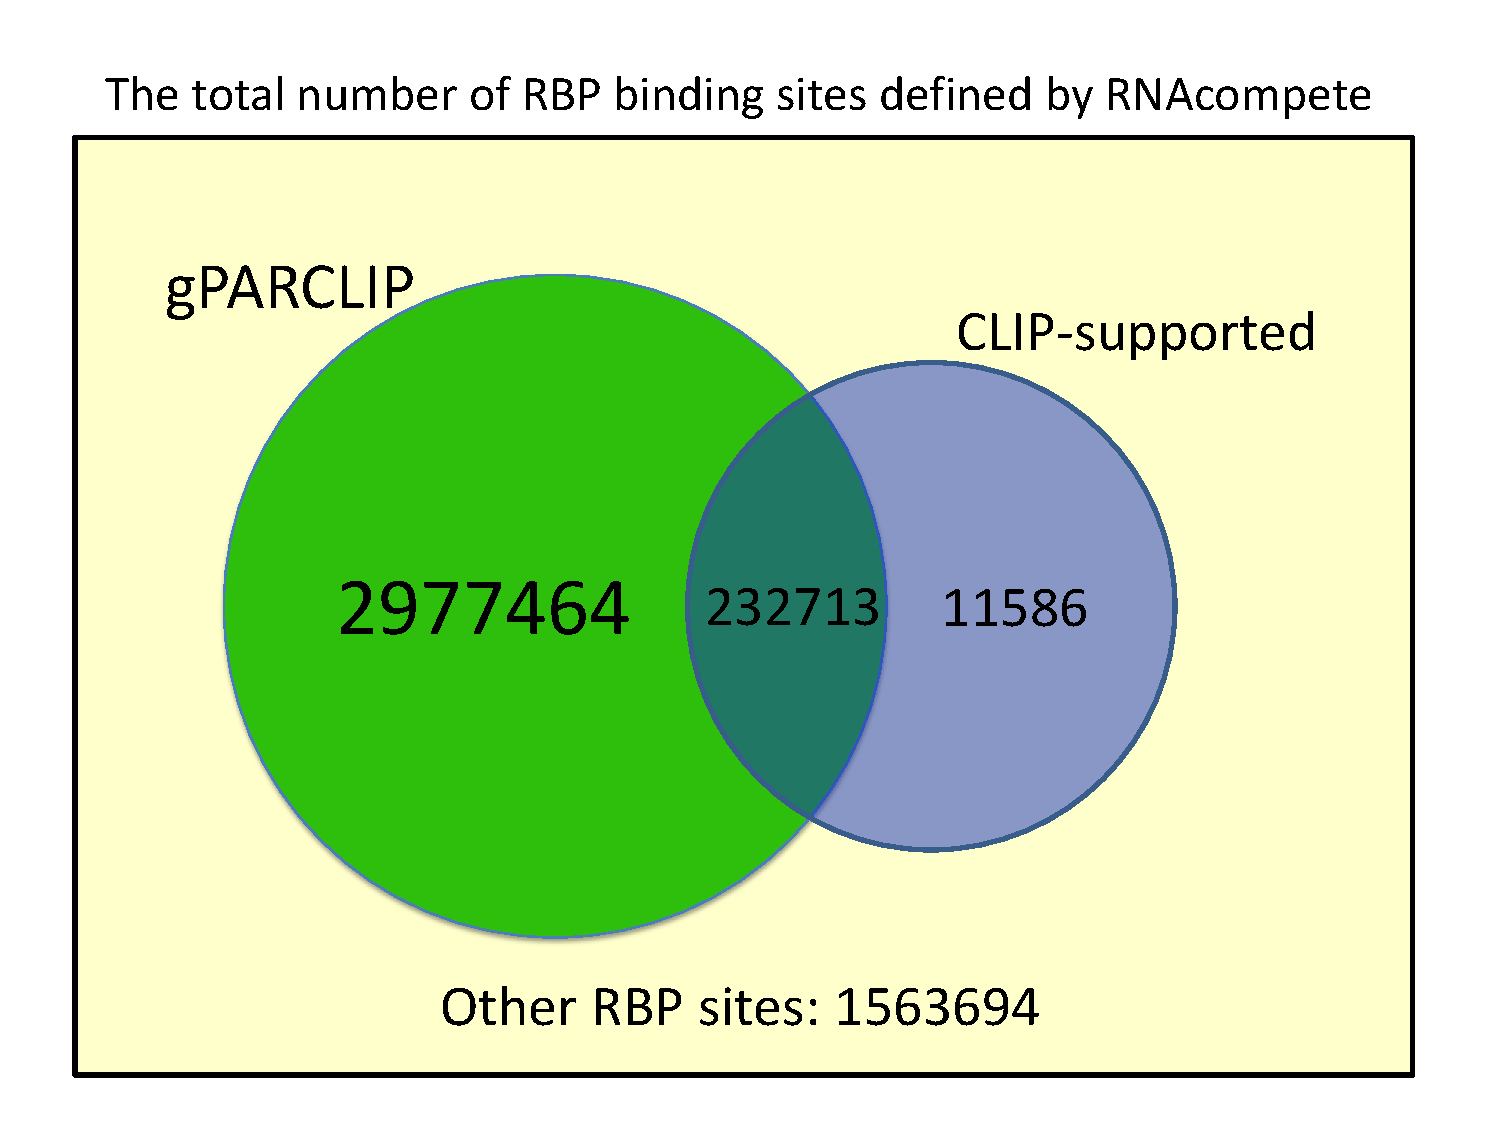
\includegraphics[width=0.5\textwidth,clip]{ch4_results_discussion/figures/rbp_sites_stat.pdf}
    \label{rbp_stat}
}
\quad
	\subfloat[]{
	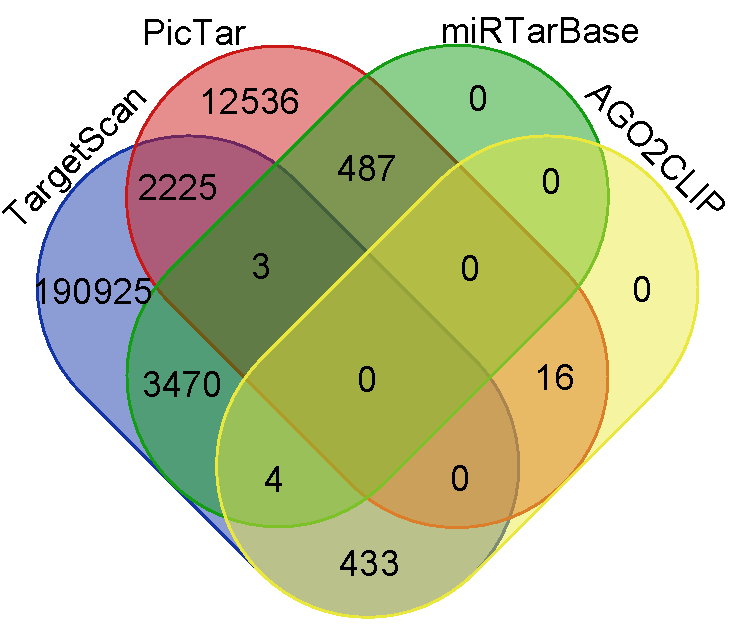
\includegraphics[width=0.5\textwidth,clip]{ch4_results_discussion/figures/mirna_sites_stat.pdf}
    \label{mirna_stat}
}
\caption[Comparison of binding sites supported by CLIP and gPARCLIP]{Venn diagram of the overlap between binding sites supported by CLIP-based techniques and gPARCLIP methods. \subref{rbp_stat} Comparison of the cumulative distribution of RBP binding sites supported by CLIP and/or gPARCLIP methods. \subref{mirna_stat} Comparison of the cumulative distribution of miRNA binding site abundance supported by any of TargetScan, PicTar, miRTarBase, and AGO2CLIP methods.}
\label{sites_statistic}
\end{figure}
%\shorthandon{=}

\clearpage
\section{Accessibility and conservation scores of binding sites of RBPs}

In this analysis, our goal was to observe the probable role of accessibility and/or conservation in differentiating RBP binding sites that are located in CLIP-determined peaks from other potential sites that are not located in CLIP-determined peaks. In order to classify potential binding sites of HuR, we scanned RNAcompete top 10 n-mers and determined following RNAcompete IDs as HuR motifs in our analysis: RNCMPT00112, RNCMPT00117, RNCMPT00136, RNCMPT00032 and RNCMPT00274. Table \ref{tbl:hur_motifs} shows the motifs for HuR RNAcompete IDs. Because RNAcompete has not been performed for PUM2, but for its Drosophila homolog Pumilio, we used the Pumilio motif as a substitute. Among the multiple RNAcompete motifs inferred for Pumilio, we chose the one (i.e., RNCMPT00104) that is most consistent with \textit{in vivo} binding data (see Supplementary Table 6 of RNAcompete paper). In addition to this motif, we also downloaded and used consensus motifs from RBPDB database for PUM1 and PUM2 proteins. PUM1 and PUM2 proteins are from same human PUF family and because of this fact they are known to have similar binding site specificities. In our upcoming analysis we used PUM1 motif to scan for PUM2 sites and vice versa. Furthermore, we scanned RNAcompete and determined RNCMPT00033 and RNCMPT00172 RNAcompete IDs as IGF2BP1-3 motifs. Besides, we considered RNAcompete ID RNCMPT00047 as the QKI motif in our analyses.

%\shorthandoff{=}
\begin{table}[H]
\centering
\setlength\extrarowheight{10pt}
\caption[RNAcompete HuR motifs]{RNAcompete HuR motifs}
\resizebox{0.65\textwidth}{!}{
\begin{tabular}{c | c | c}
RNAcompete ID & IUPAC & Motif \\ [0.7ex] 
\hline
RNCMPT00112 & UUWGUUU & \begin{center}
\includegraphics[scale = 0.25]{ch4_results_discussion/figures/hur_motif/RNCMPT00112.png}\end{center} \\[0.5ex]

RNCMPT00117 & UUURKUU & \begin{center}
\includegraphics[scale = 0.25]{ch4_results_discussion/figures/hur_motif/RNCMPT00117.png}\end{center} \\[0.5ex]

RNCMPT00274 & UUUUUUK & \begin{center}
\includegraphics[scale = 0.25]{ch4_results_discussion/figures/hur_motif/RNCMPT00274.png}\end{center} \\[0.5ex]

RNCMPT00032 & UUDUUUU & \begin{center}
\includegraphics[scale = 0.25]{ch4_results_discussion/figures/hur_motif/RNCMPT00032.png}\end{center} \\[0.5ex]

RNCMPT00136 & UUKRUUU & \begin{center}
\includegraphics[scale = 0.25]{ch4_results_discussion/figures/hur_motif/RNCMPT00136.png}\end{center} \\

\end{tabular} %
}
\label{tbl:hur_motifs}
\end{table}
%\shorthandon{=}

Our hypothesis in this analysis was that experimentally validated sites should have higher accessibility and conservation scores compared to other sites. We classified the transcripts into two groups based on CLIP-determined peaks. The first group contained binding sites which reside in CLIP peaks (i.e., CLIP-supported sites) and the other group contained binding sites which are not CLIP-supported (i.e., other sites). Next we compared the cumulative distribution of accessibility and conservation scores between these two groups. (see Figures ~\ref{HuR_accessibility}, ~\ref{HuR_conservation}, and ~\ref{PUM_accessibility_and_conserv})

%\shorthandoff{=}
\begin{figure}[H]
	\centering
   	\subfloat[]{
   	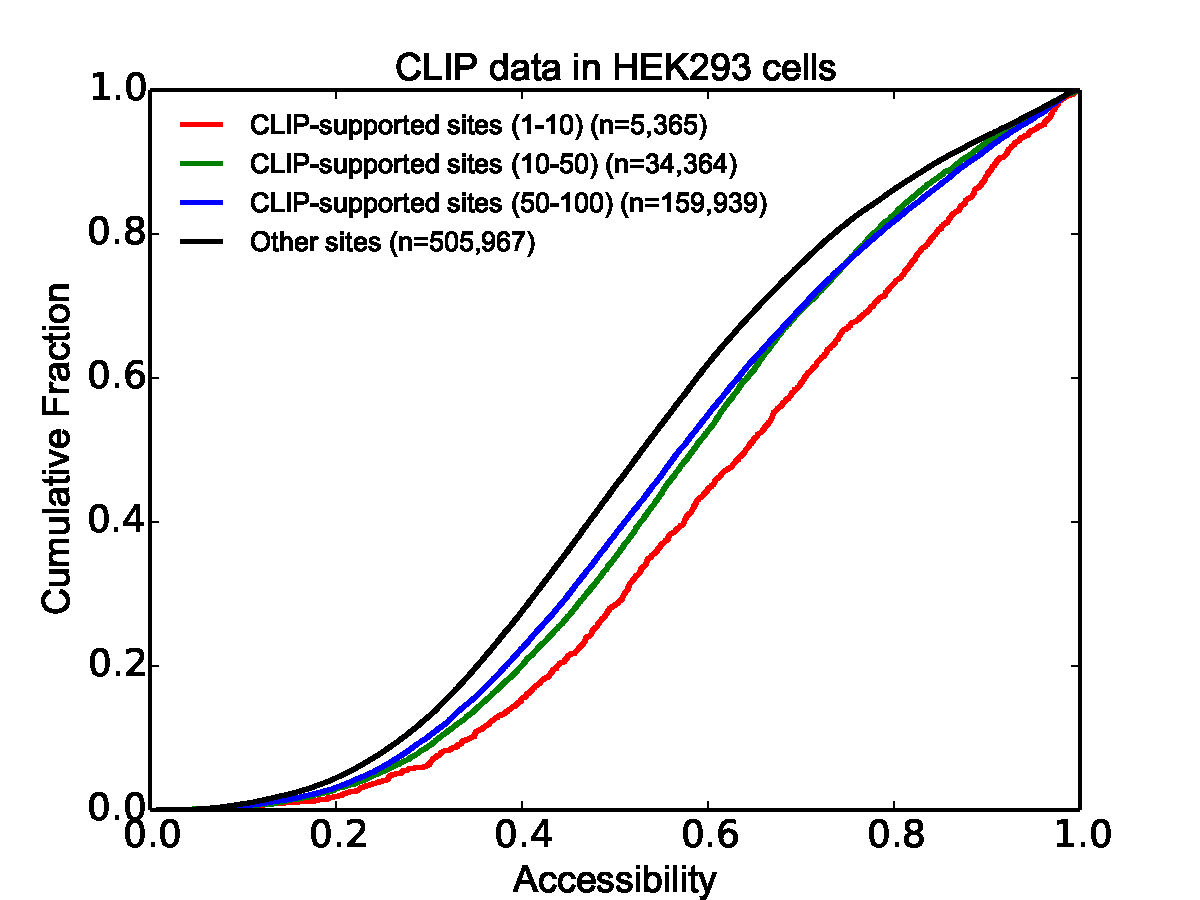
\includegraphics[width=0.55\textwidth,clip]{ch4_results_discussion/figures/Figure2a.pdf}
    \label{HuR_accessibility_HEK293}
}
\quad
	\subfloat[]{
	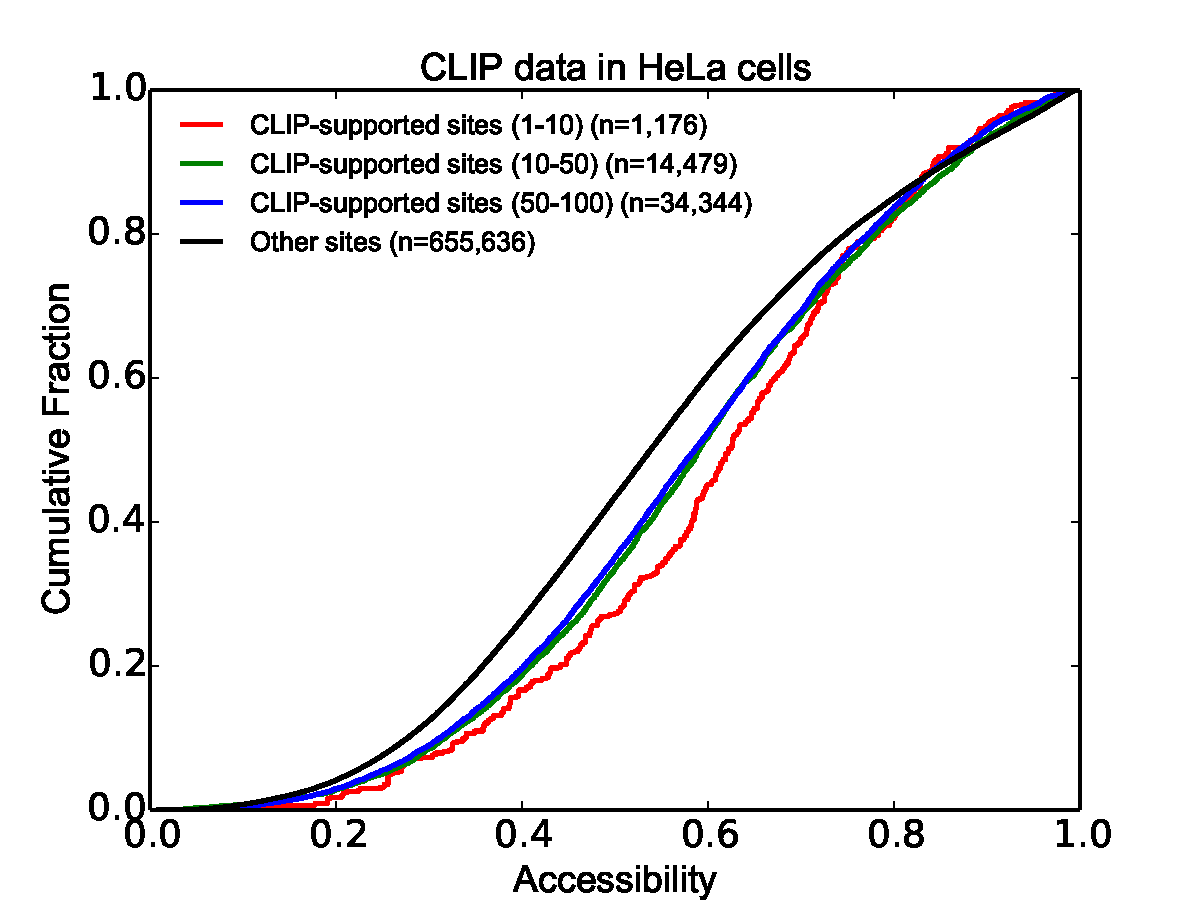
\includegraphics[width=0.55\textwidth,clip]{ch4_results_discussion/figures/Figure2b.pdf}
    \label{HuR_accessibility_HeLa}
}
\caption[Accessibility of HuR protein]{Comparison of CLIP-supported and not CLIP-supported sites (i.e., other sites) of HuR in terms of accessibility. For accessibility analysis, CLIP-supported sites are classified into different groups based on the scores of the peaks that they are located in. \subref{HuR_accessibility_HEK293} Cumulative density fraction of accessibility scores of CLIP-supported sites and other sites where CLIP experiment is performed in HEK293 cells. \subref{HuR_accessibility_HeLa} Cumulative density fraction of accessibility scores of CLIP-supported sites and other sites where CLIP experiment is performed in HeLa cells.}
\label{HuR_accessibility}
\end{figure}
%\shorthandon{=}

Either considering PARCLIP data from HEK293 cells \cite{hafner_10} or HeLa cells \cite{lebedeva_11}, we noticed that the CLIP-supported HuR sites are more accessible. This result is in accordance with previous studies \cite{hur_accessibility}. On the other hand, we grouped these CLIP-supported sites according to their peak score (i.e. percentiles downloaded from doRINA database) to see their effect in much detail and as expected, we noticed that the sites that reside in peaks with higher scores are more accessible compared to other CLIP-supported sites (MannWhitneyU two-tailed test P-value = $1.1E-203$ for HEK293 cells and P-value = $4.5E-35$ for HeLa cells)(See Figures \ref{HuR_accessibility_HEK293} and \ref{HuR_accessibility_HeLa}). Next, we repeated the same type of analysis to investigate the effect of PhastCons conservation scores on CLIP-supported sites. We observed that conservation scores significantly differ between CLIP-supported sites and other sites of HuR protein either considering HEK293 CLIP data (P-value = $6.1E-16$) or HeLa CLIP data (P-value $\approx 0$) (See Figures \ref{HuR_conservation_HEK293} and \ref{HuR_conservation_HeLa} respectively). The difference is much more significant in HeLa cells compared to HEK293 cells.

Figure \ref{PUM_accessibility} shows that PUM1(2) experimentally validated sites are less accessible compared to other sites (P-value = $1.74E-10$). PUM1 is known to bind single-stranded motifs \cite{wang_02} and to downregulate its target mRNAs. PUM2 is expected to have a similar binding preferences as PUM1. We considered PUM2 CLIP-supported sites for this analysis. However, as \ref{PUM_accessibility} shows, we observed the opposite where PUM2 CLIP-supported sites are less accessible compared to other sites. In order to investigate it in further detail, we distinguished CLIP-supported sites according to their peak scores. We observed that sites in the high scoring peaks (percentile 1-10) are less accessible compared to sites located in low scoring peaks (Percentile 50-100) with a P-value = $0.002$. Figure \ref{PUM_accessibility} shows the accessibility score distribution of sites in distinguished groups. In case of conservation, as shown in Figure ~\ref{PUM_conservation}, CLIP-supported sites are significantly more conserved than other sites (P-value $\approx 0$).

\clearpage
%\shorthandoff{=}
\begin{figure}[H]
	\centering
	\subfloat[]{
	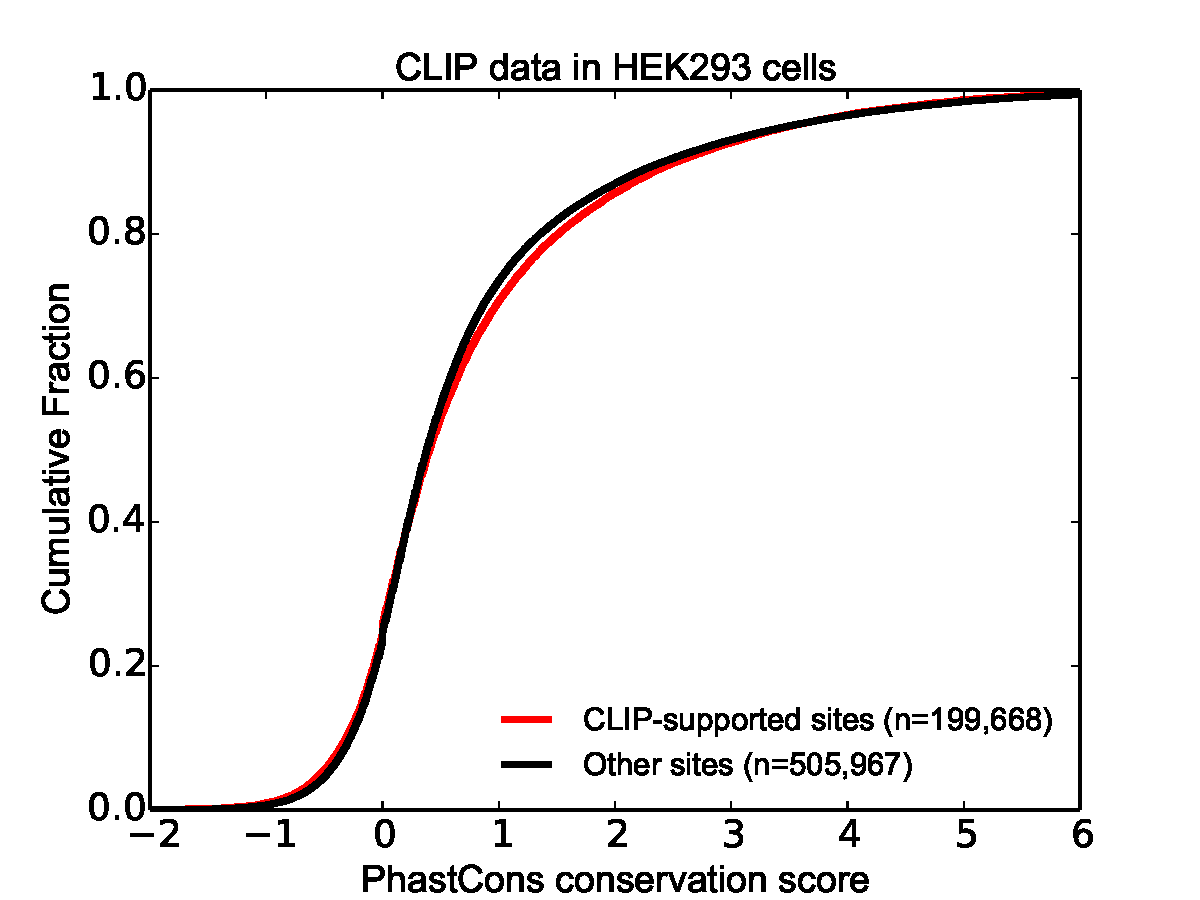
\includegraphics[width=0.7\textwidth,clip]{ch4_results_discussion/figures/Figure2c.pdf}
    \label{HuR_conservation_HEK293}
}
\quad
	\subfloat[]{
    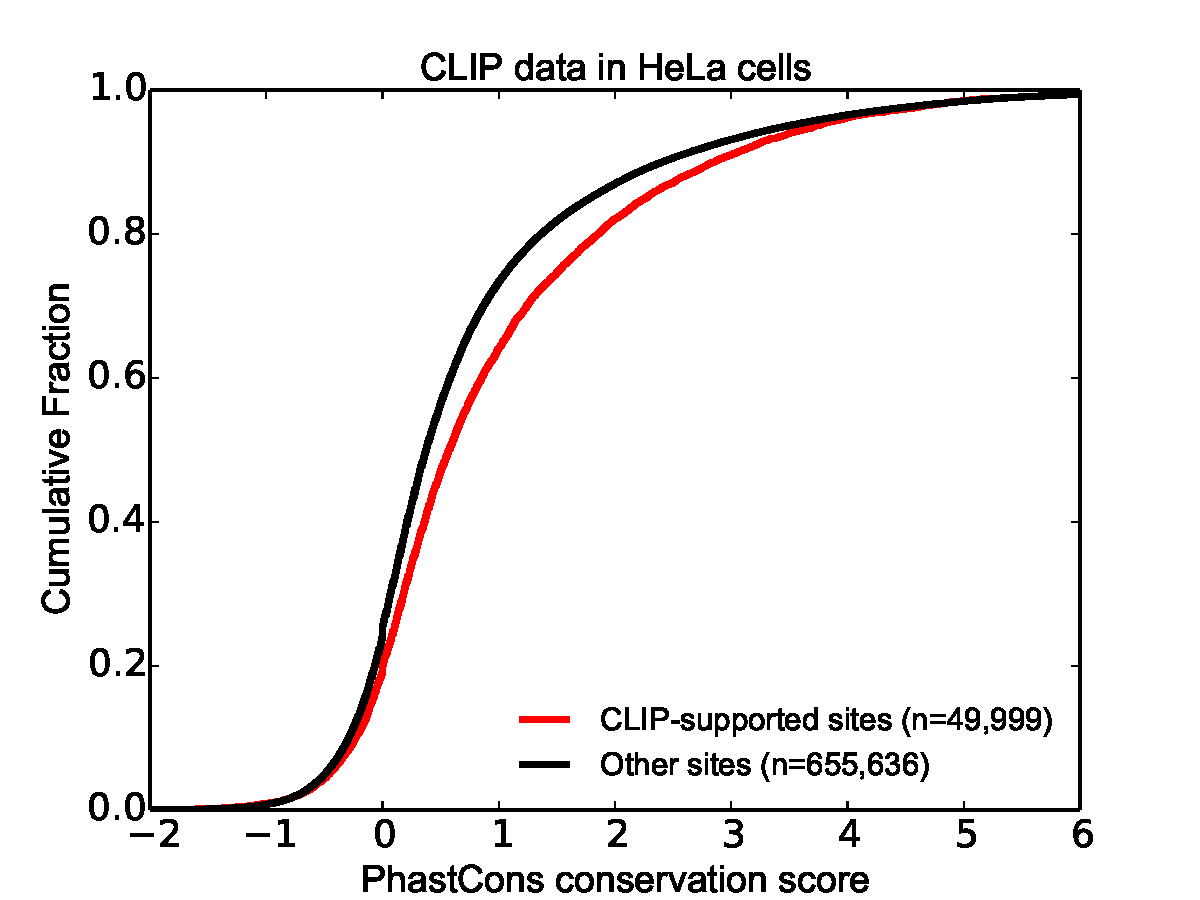
\includegraphics[width=0.7\textwidth,clip]{ch4_results_discussion/figures/Figure2d.pdf}
    \label{HuR_conservation_HeLa}
}
\caption[Conservation scores of HuR protein]{Comparison of CLIP-supported sites and not CLIP-supported sites (i.e., other sites) of HuR in terms of conservation scores. \subref{HuR_conservation_HEK293} Cumulative density fraction of conservation scores of CLIP-supported sites and other sites where CLIP experiment is performed in HEK293 cells. \subref{HuR_conservation_HeLa} Cumulative density fraction of conservation scores of CLIP-supported sites and other sites where CLIP experiment is performed in HeLa cells.}
\label{HuR_conservation}
\end{figure}
%\shorthandon{=}

\clearpage

%\shorthandoff{=}
\begin{figure}[H]
	\centering
	\subfloat[]{
    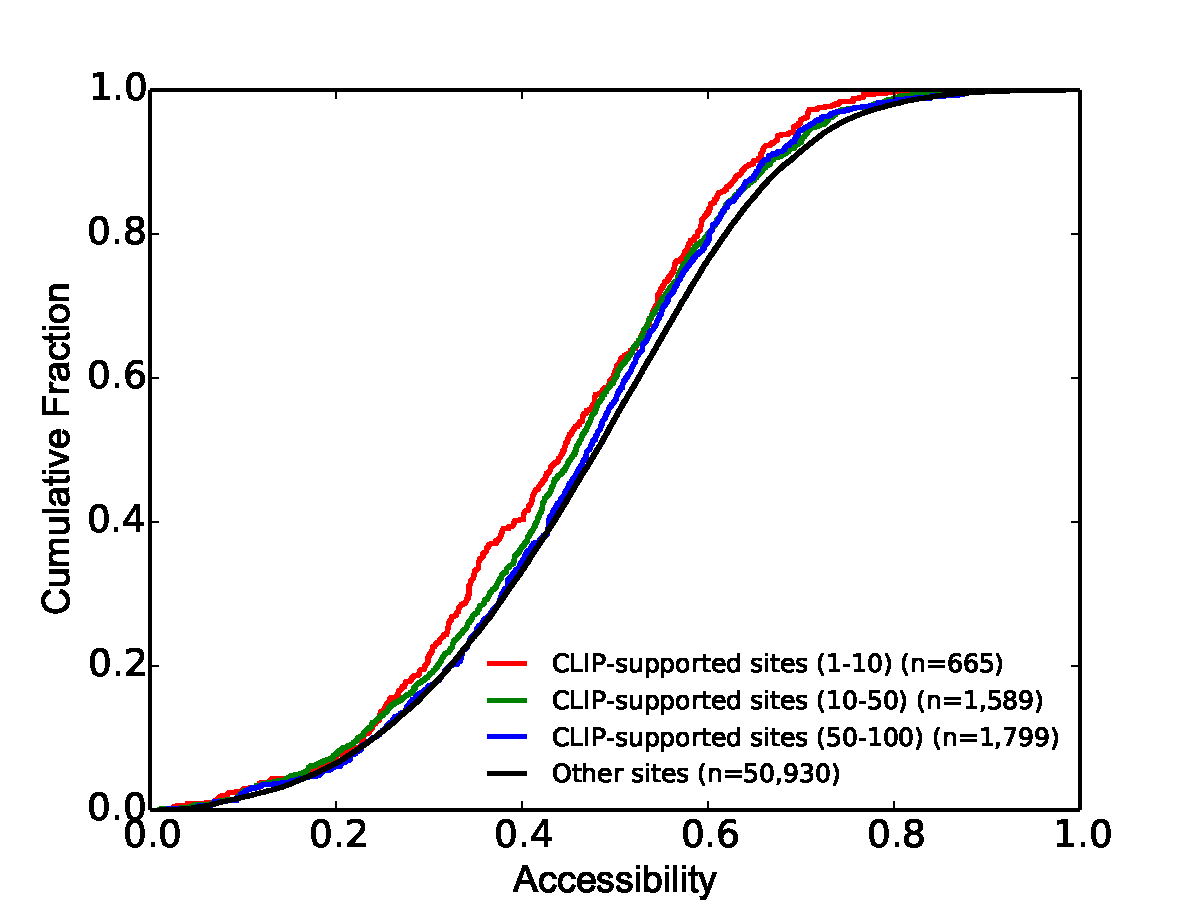
\includegraphics[width=0.7\textwidth,clip]{ch4_results_discussion/figures/Figure3a}
    \label{PUM_accessibility}
}
\quad
	\subfloat[]{
	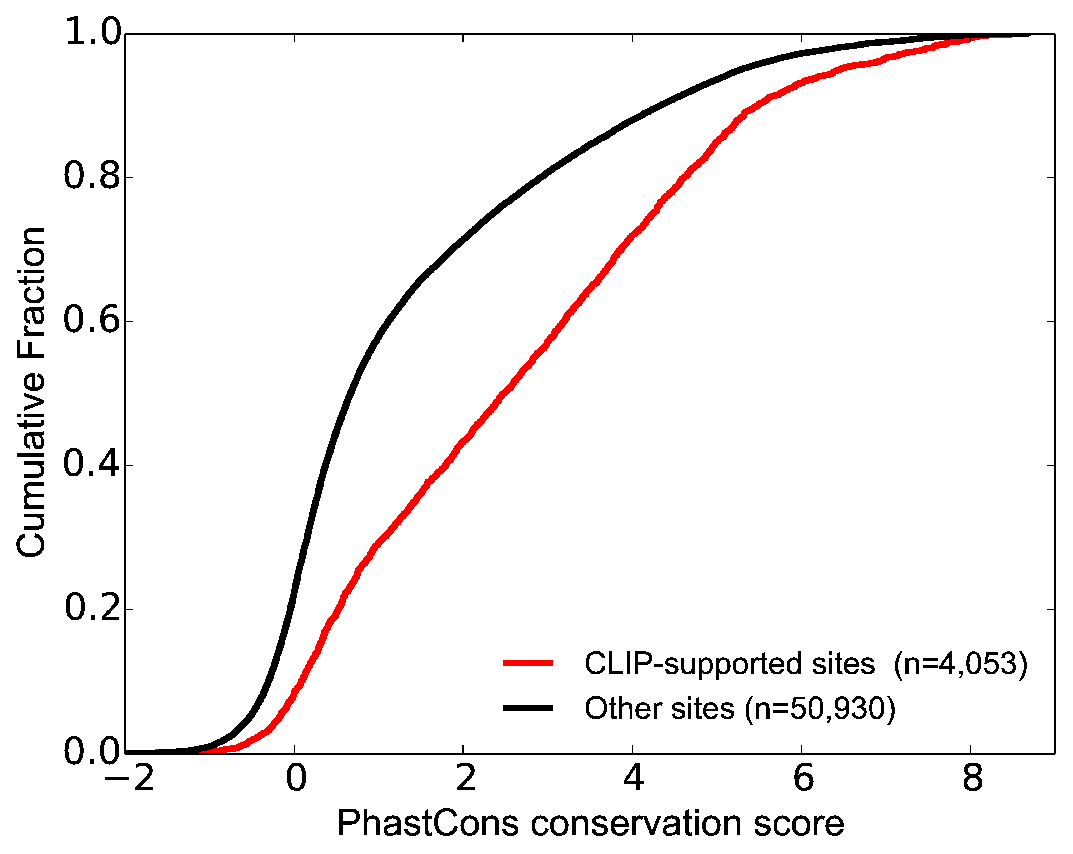
\includegraphics[width=0.7\textwidth,clip]{ch4_results_discussion/figures/Figure3b}
    \label{PUM_conservation}
}
\caption[Accessibility and conservation scores of PUM protein]{Comparison between CLIP-supported and other sites of PUM1(2) in terms of accessibility and conservation. \subref{PUM_accessibility} Cumulative density fraction of accessibility scores of CLIP-supported sites and other sites. \subref{PUM_conservation} Cumulative density fraction of conservation scores of CLIP-supported sites and other sites.}
\label{PUM_accessibility_and_conserv}
\end{figure}
%\shorthandon{=}

\clearpage
Furthermore, we repeated this analysis with QKI and IGF2BP1-3 RBPs. Figure \ref{IGF2BP_accessibility_and_conserv} shows that experimentally validated IGF2BP1-3 sites are more conserved compared to other sites (P-value = $4.4E-16$). On the other hand, in case of accessibility, we observed that CLIP-supported binding sites of IGF2BP1-3 are less accessible (P-value = $4.4E-16$). Figure \ref{QKI_accessibility_and_conserv} shows the comparison between CLIP-supported and other binding sites of QKI. We observed that CLIP-supported QKI binding sites are significantly more conserved compared to other QKI binding sites (P-value = $7.5E-09$). Besides, CLIP-supported QKI binding sites are more accessible (P-value = $2.7E-03$).

%\shorthandoff{=}
\begin{figure}[H]
	\centering
	\subfloat[]{
    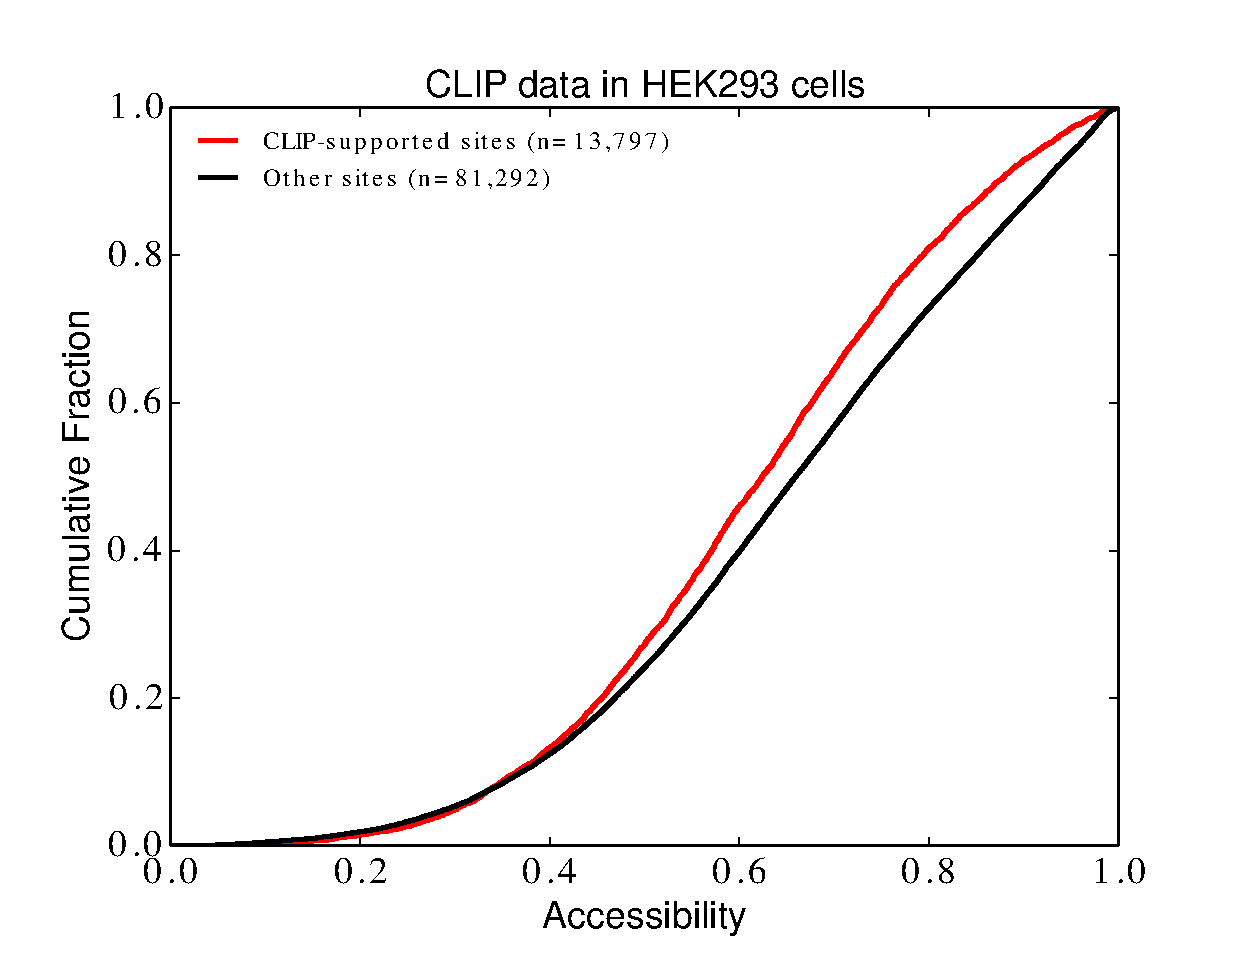
\includegraphics[width=0.65\textwidth,clip]{ch4_results_discussion/figures/IGF2BP_rnaplfold_accessibility_analysis_HEK293_2015_8_28.eps}
    \label{IGF2BP_accessibility}
}
\quad
	\subfloat[]{
	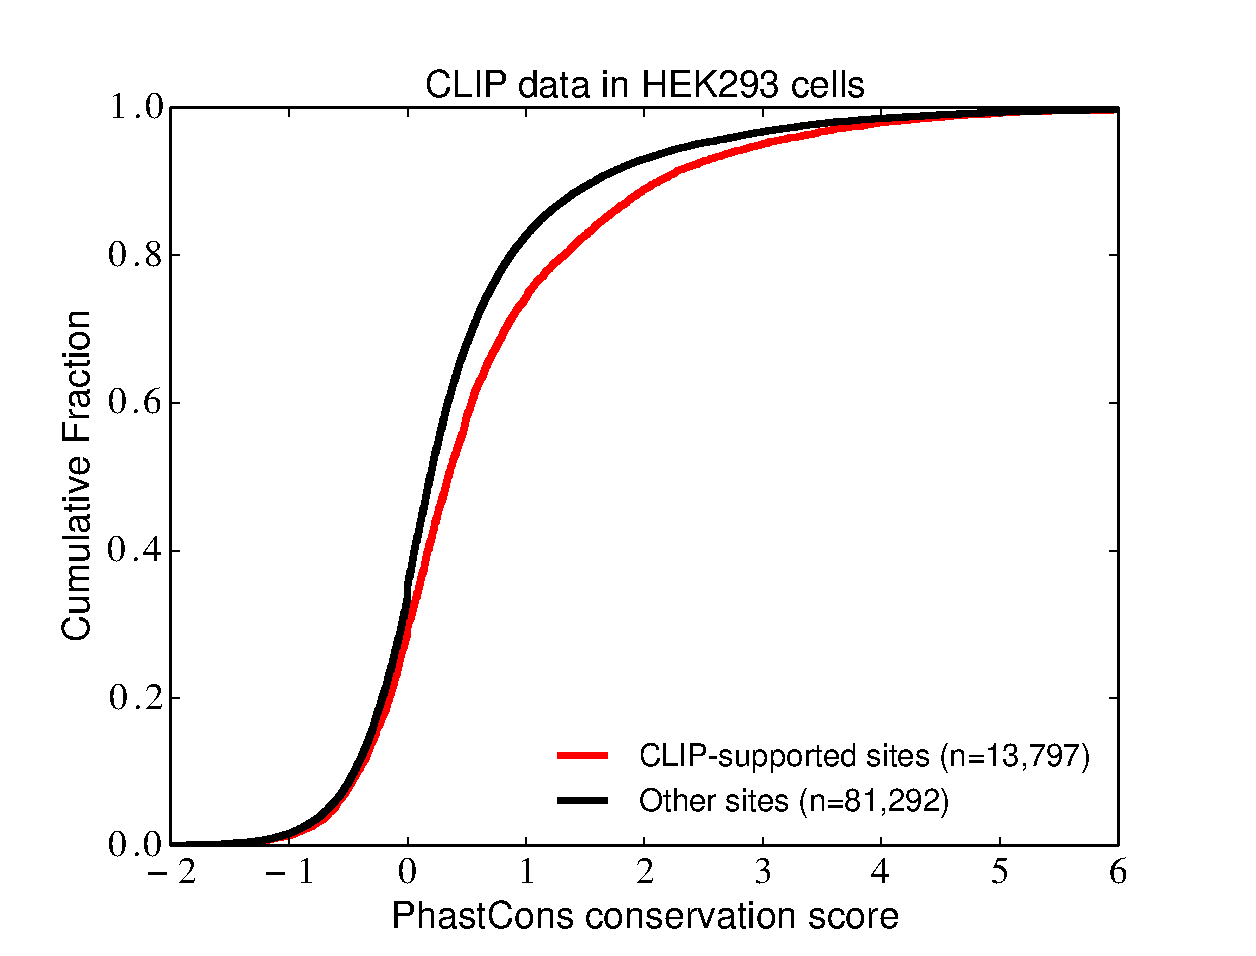
\includegraphics[width=0.65\textwidth,clip]{ch4_results_discussion/figures/IGF2BP_conservation_effect_HEK293_Aug27.eps}
    \label{IGF2BP_conservation}
}
\caption[Accessibility and conservation scores of IGF2BP1-3 protein]{Comparison between CLIP-supported and other sites of IGF2BP1-3 in terms of accessibility and conservation. \subref{IGF2BP_accessibility} Cumulative density fraction of accessibility scores of CLIP-supported sites and other sites. \subref{IGF2BP_conservation} Cumulative density fraction of conservation scores of CLIP-supported sites and other sites.}
\label{IGF2BP_accessibility_and_conserv}
\end{figure}
%\shorthandon{=}


%\shorthandoff{=}
\begin{figure}[H]
	\centering
	\subfloat[]{
    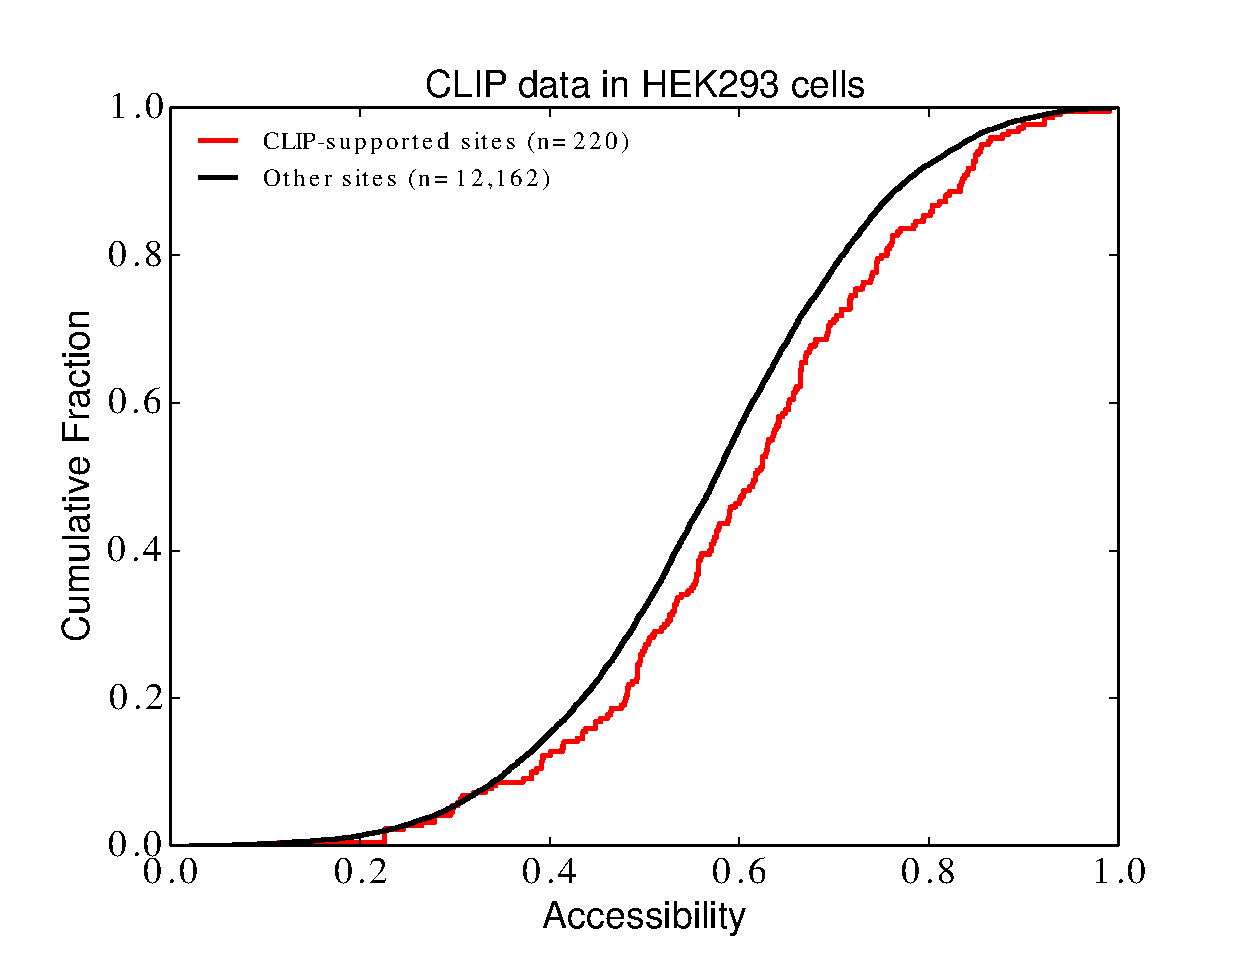
\includegraphics[width=0.65\textwidth,clip]{ch4_results_discussion/figures/QKI_rnaplfold_accessibility_analysis_HEK293_2015_8_28.eps}
    \label{QKI_accessibility}
}
\quad
	\subfloat[]{
	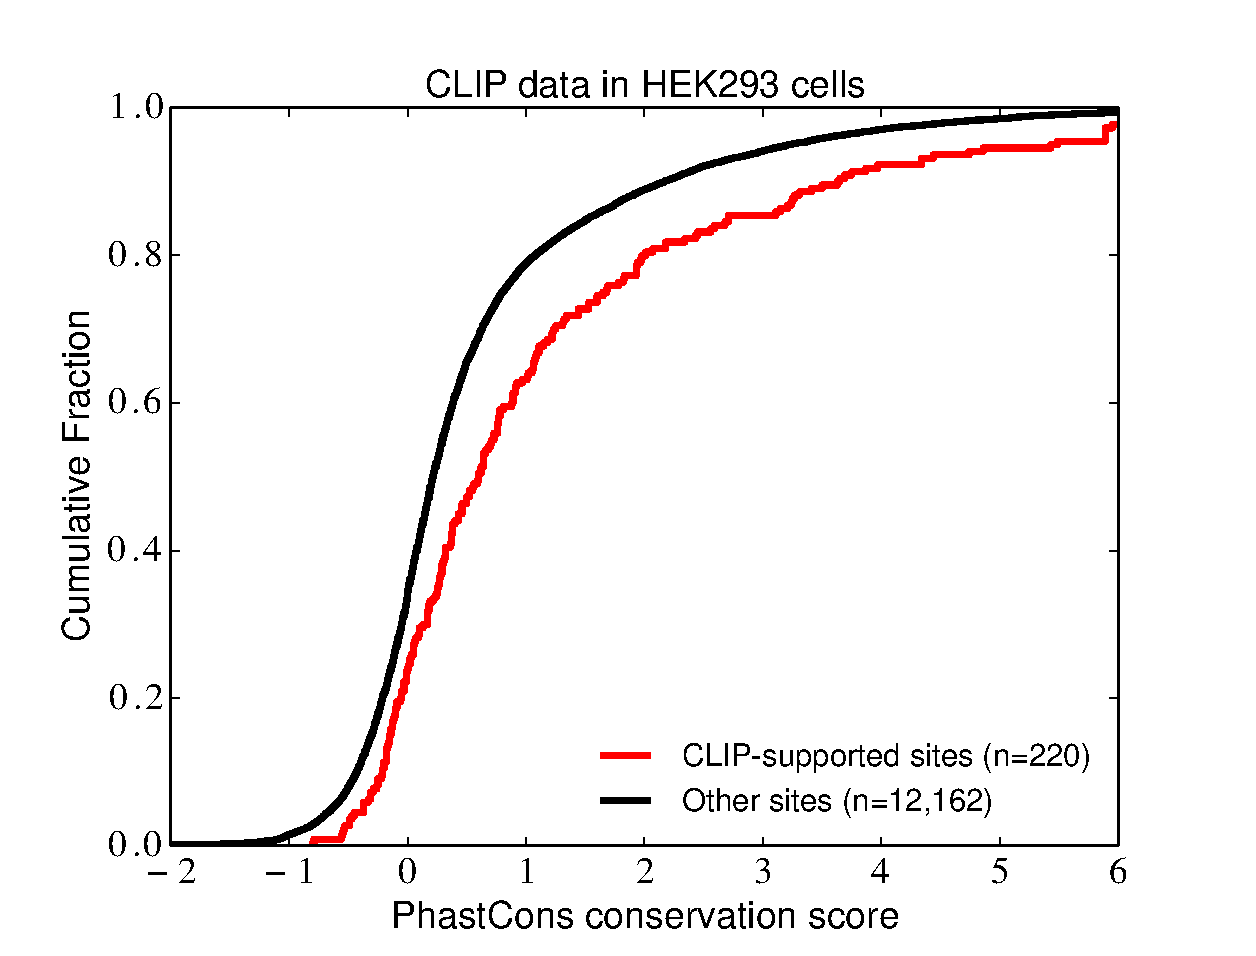
\includegraphics[width=0.65\textwidth,clip]{ch4_results_discussion/figures/QKI_conservation_effect_HEK293_Aug27.eps}
    \label{QKI_conservation}
}
\caption[Accessibility and conservation scores of QKI protein]{Comparison between CLIP-supported and other sites of QKI in terms of accessibility and conservation. \subref{QKI_accessibility} Cumulative density fraction of accessibility scores of CLIP-supported sites and other sites. \subref{QKI_conservation} Cumulative density fraction of conservation scores of CLIP-supported sites and other sites.}
\label{QKI_accessibility_and_conserv}
\end{figure}
%\shorthandon{=}

As discussed before, we distinguished CLIP-supported sites of PUM2 and HuR according to their CLIP score in accessibility analysis. However, in case of QKI and IGF2BP1-3 binding sites, we considered all CLIP-supported binding sites in one single group. That is because there are little amount of CLIP-supported binding sites and distinguishing them into several groups makes it harder to investigate the effect of CLIP-supported sites in case of accessibility and conservation.

Generally, we investigated the effect of CLIP-supported sites of RBPs in case of accessibility and conservation. In the following section, we utilize knockdown datasets to further investigate effect of CLIP-supported sites on expression of mRNAs.

%change the title
\section{Analysis of knockdown datasets}

In this series of analyses we aim to assess the effect of CLIP-supported sites and consequences of competition between particular RBPs and other factors on the expression of mRNAs. We repeated this analysis for HuR, QKI, and IGF2BP1-3 proteins for which knockdown datasets are available. We used log fold expression changes of transcripts upon HuR depletion in HEK293 and HeLa cells from \cite{mukharjee_11} and \cite{lebedeva_11} respectively. As for QKI and IGF2BP1-3, we used knockdown datasets from Hafner et al. in HEK293 cells \cite{hafner_10}.

Mukharjee et al. \cite{mukharjee_11} has shown that even transcripts with only intronic HuR sites still show reduced expression upon HuR knockdown in HEK293 cells. Our aim is to understand the function of HuR sites in 3'UTs. Therefore, we decided to filter out those transcripts that contain intronic HuR sites in order to avoid their concealed effects throughout the following analyses related to HuR.

\subsection{Effect of CLIP-supported sites on transcripts expression}
 
In this analysis our aim was to investigate the effect of experimentally validated RBP sites on expression of transcripts compared to the effect of other sites of that RBP which are not CLIP-supported. Expression log fold changes upon knockdown of a single factor provides valuable information about that factor's behavior. HuR increases the stability of its target mRNAs. Therefore, we expected to see higher destabilization in transcripts containing experimentally validated HuR sites compared to other sites in which HuR was knocked down.

In order to illustrate our expectations, we classified transcripts into three groups: (i) those that have at least one CLIP-supported HuR site; (ii) those that have one or more predicted HuR sites but none of them are CLIP-supported; and (iii) those that have no HuR sites at all. Figure ~\ref{HuR_CLIPsupport} shows the cumulative distribution of LFC of the transcripts belonging to these groups. Considering the distribution of LFC of the transcripts having no HuR sites at all as our baseline, we observed that transcripts in the first group are more destabilized upon HuR Knockdown compared to those transcripts in the second group. (Figure \ref{HuR_CLIPsupport_HEK293}, P-value = $1.8E-81$) and  (Figure \ref{HuR_CLIPsupport_HeLa}, P-value = $5.2E-05$)

\clearpage
%\shorthandoff{=}
\begin{figure}[H]
	\centering
	\subfloat[]{
	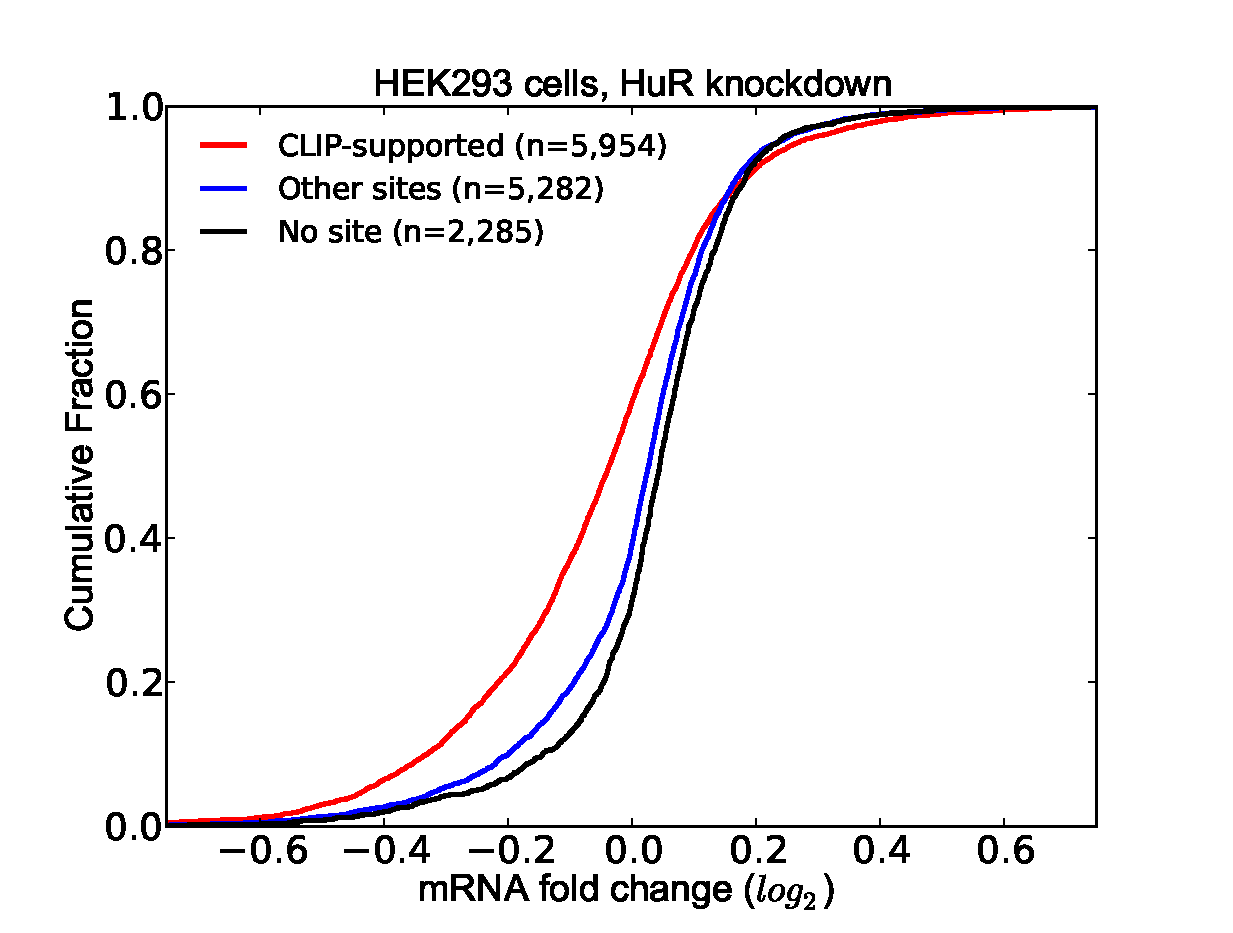
\includegraphics[width=0.65\textwidth,clip]{ch4_results_discussion/figures/Mukharjee_HEK293_CLIP_supported_notsupported_HuRAll_ConsTHNone_Excluded_allgroups_2015_8_20.eps}
    \label{HuR_CLIPsupport_HEK293}
}
\quad
	\subfloat[]{
    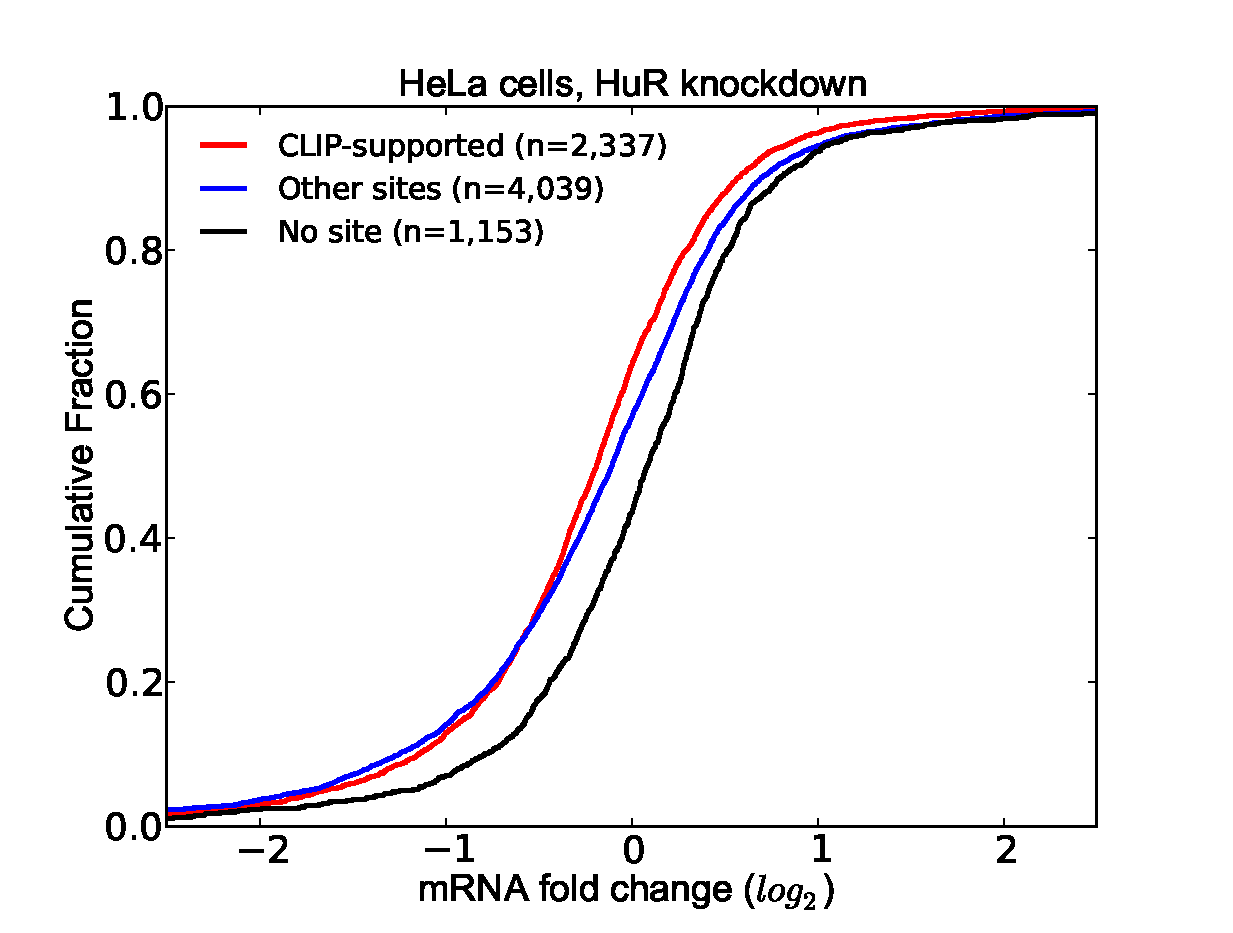
\includegraphics[width=0.65\textwidth,clip]{ch4_results_discussion/figures/Lebedeva_HeLa_CLIP_supported_notsupported_HuRAll_ConsTHNone_Excluded_allgroups_2015_8_20.eps}
    \label{HuR_CLIPsupport_HeLa}
}
\caption[Comparison between CLIP-supported HuR sites and Other sites]{Comparison of the effect of HuR depletion on transcripts that contain CLIP-supported HuR sites against those that do not contain CLIP-supported HuR sites. X axis shows the log fold change of transcripts upon HuR depletion. \subref{HuR_CLIPsupport_HEK293} Response of mRNAs to the loss of HuR in HEK293 cells. \subref{HuR_CLIPsupport_HeLa} Response of mRNAs to the loss of HuR in HeLa cells. }
\label{HuR_CLIPsupport}
\end{figure}
%\shorthandon{=}

We also repeated this analysis with QKI and IGF2BP1-3 RBPs in order to further approve our findings with HuR. Figure \ref{QKI_CLIP-supported} shows the comparison between expression of transcripts that contain CLIP-supported QKI binding sites and those that do not contain CLIP-supported QKI binding sites in case of QKI knockdown. Hafner et al. \cite{hafner_10} provides two siRNA dataset for QKI knockdown and here we calculated the average values from these two siRNA knockdown datasets and used it to investigate the effect of CLIP-supported QKI binding sites on expression of their target mRNAs. 

%\shorthandoff{=}
\begin{figure}[H]
	\centering
	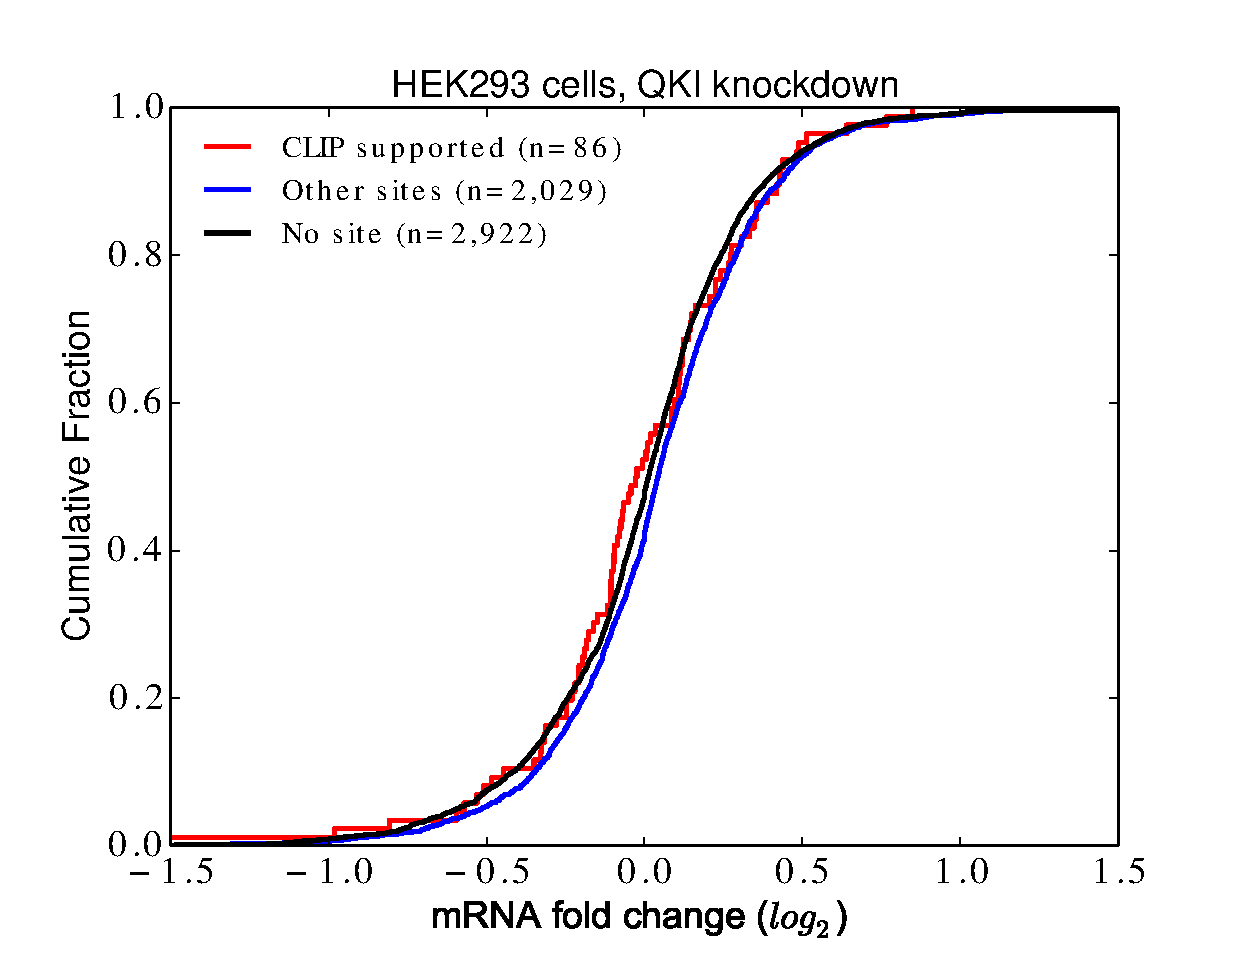
\includegraphics[width=0.8\textwidth,clip]{ch4_results_discussion/figures/Hafner_HEK293_QKI_SetAB_avg_CLIP_supported_notsupported_THNone_corrected_2015_8_28.eps}
\caption[Comparison between CLIP-supported QKI sites and other sites]{Comparison of the effect of QKI depletion on transcripts that contain CLIP-supported QKI sites against those that do not contain CLIP-supported QKI sites. X axis shows the log fold change of transcripts upon QKI depletion. It shows the response of mRNAs to the loss of QKI in HEK293 cells}
\label{QKI_CLIP-supported}
\end{figure}
%\shorthandon{=}

%\shorthandoff{=}
\begin{figure}[H]
	\centering
	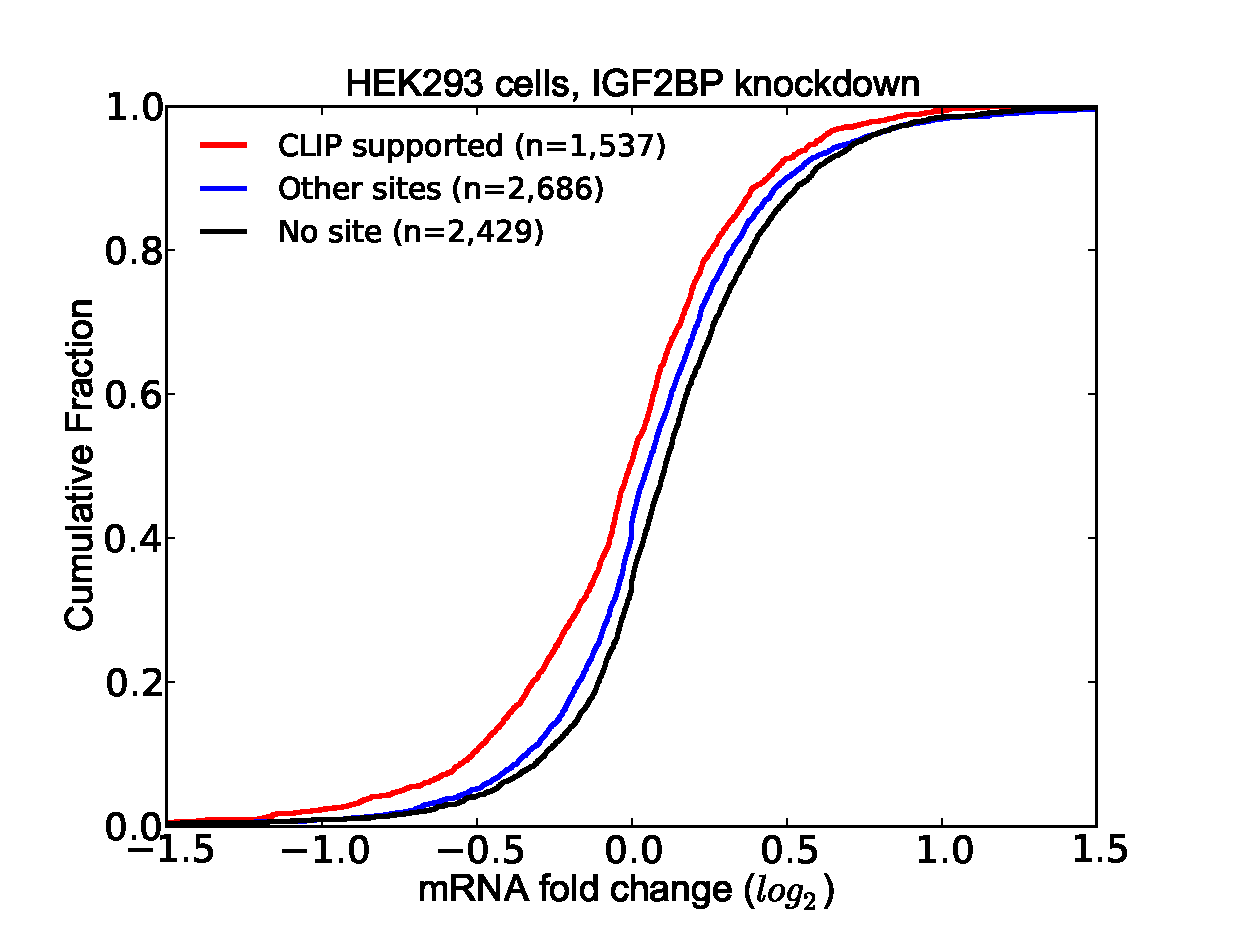
\includegraphics[width=0.8\textwidth,clip]{ch4_results_discussion/figures/Hafner_HEK293_IGF2BP1-2_CLIP_supported_notsupported_THNone_2015_8_28_corrected.eps}
\caption[Comparison between CLIP-supported IGF2BP1-3 sites and other sites]{Comparison of the effect of IGF2BP1-3 depletion on transcripts that contain CLIP-supported IGF2BP1-3 sites against those that do not contain CLIP-supported IGF2BP1-3 sites. X axis shows the log fold change of transcripts upon IGF2BP1-3 depletion. It shows the response of mRNAs to the loss of IGF2BP1-3 in HEK293 cells}
\label{IGF_CLIP-supported}
\end{figure}
%\shorthandon{=}

As figure \ref{QKI_CLIP-supported} shows, we couldn't observe a net effect on the expression of QKI target mRNAs. There is no significant difference between log fold change of transcripts in groups 1 and 2 (P-value = $0.17$). Indeed, the roles of QKI on splicing is well established; however, its effect to stability is not well determined. Hafner et al. \cite{hafner_10} has found that QKI decreases stability. On the other hand, another study by Teplova et al. \cite{teplova_2013} have analyzed the same datasets and showed that QKI increases stability. Therefore, we decided to exclude this RBP from our analyses.

Figure \ref{IGF_CLIP-supported} shows the effect of CLIP-supported IGF2BP1-3 sites on abundance of its target mRNAs. IGF2BP1-3 is known to increase the stability of its target mRNAs. Indeed, we observed that the transcripts which contain CLIP-supported IGF2BP1-3 binding sites are more destabilized upon IGF2BP1-3 knockdown compared to transcripts in second group (P-value = $6.84E-14$).

\subsection{The effect of competition to HuR function}

Transcripts are known to be occupied by several RBPs and miRNAs concurrently. In this analysis, we aim to determine the outcome of HuR competition with other factors. We suppose that two factors may involve in a competitive situation when they both target the same region. If the binding sites of these factors overlap with each other, we consider them as putative competitors. As such, In the initial step, we defined a HuR site to be overlapping if there was another factor (RBP or miRNA) which targets the same region. Next, we classified the transcripts into three groups: (i) transcripts that have at least one CLIP-supported HuR site that is not overlapping with any other site (no competition); (ii) transcripts that have at least one CLIP-supported HuR site but all HuR sites including the CLIP-supported ones are overlapping with sites of other factors (competition); and (iii) transcripts that have no HuR site at all. In order to filter out the effect of transcripts that contain intronic HuR sites, we excluded them in the initial step. Figure \ref{HuR_competition} illustrates that transcripts in \textit{no competition} group are destabilized more after HuR knockdown compared to the transcripts in \textit{competition} group. This observation holds true for HuR knockdown dataset both from HEK293 and HeLa cell lines. (P-value = $1.4E-05$ and $7.5E-05$ respectively)

\clearpage
%\shorthandoff{=}
\begin{figure}[H]
	\centering
	\subfloat[]{
	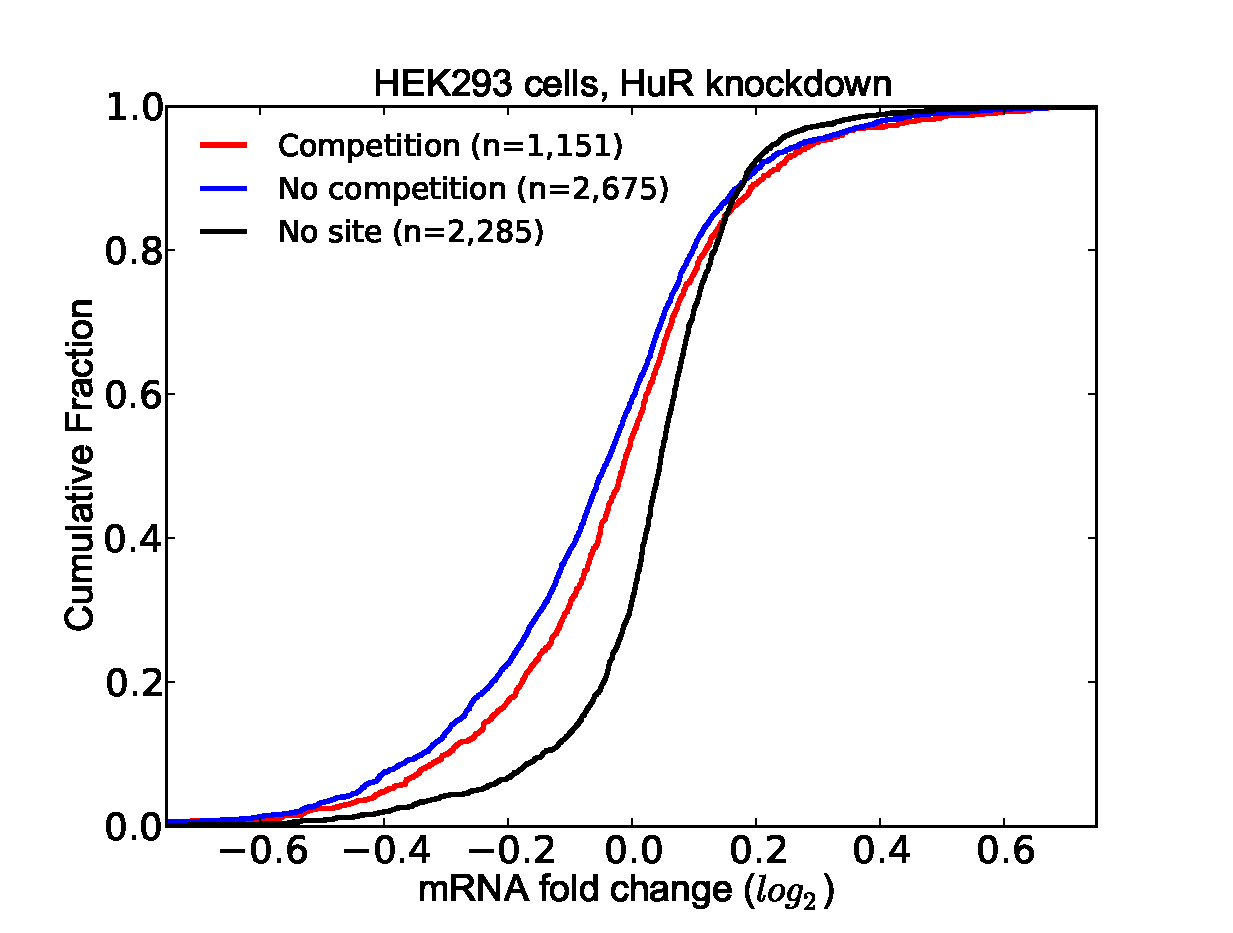
\includegraphics[width=0.75\textwidth,clip]{ch4_results_discussion/figures/HuR_Mukharjee_HEK293_competition_allsites_ConsTHNone_overlap_ExcludedAll_Expressedtop1002015_8_20.eps}
    \label{HuR_competition_HEK293}
}
\quad
	\subfloat[]{
    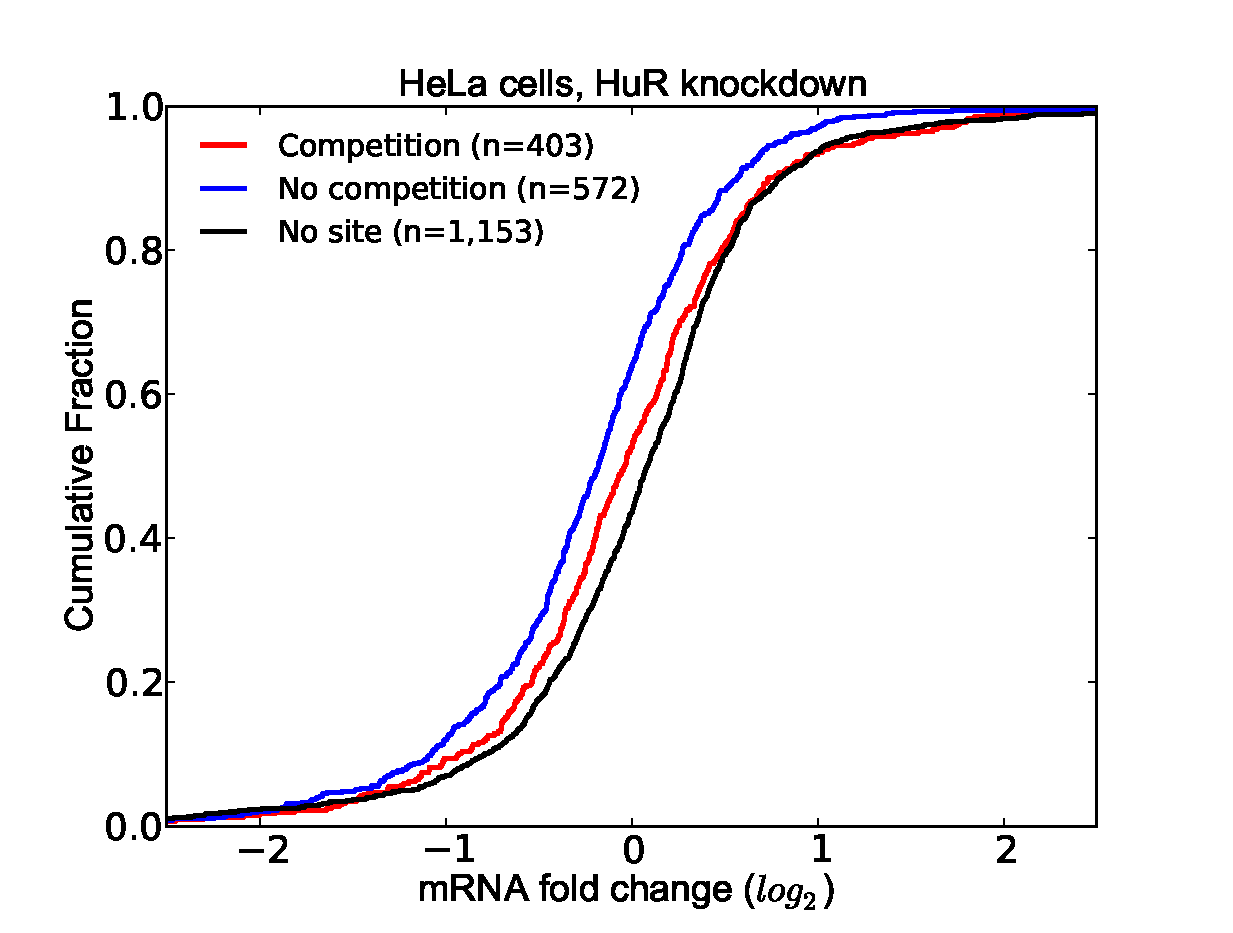
\includegraphics[width=0.75\textwidth,clip]{ch4_results_discussion/figures/HuR_Lebedeva_HeLa_competition_allsites_ConsTHNone_overlap_ExcludedAll_Expressedtop1002015_8_20.eps}
    \label{HuR_competition_HeLa}
}
\caption[Competition effect on HuR sites]{The effect of competition between HuR binding sites and other factors binding sites on expression of mRNAs. \subref{HuR_competition_HEK293} Response of mRNAs to the loss of HuR in HEK293 cells. \subref{HuR_competition_HeLa} Response of mRNAs to the loss of HuR in HeLa cells.}
\label{HuR_competition}
\end{figure}
%\shorthandon{=}

Here, we assess the effect of competition of HuR binding sites with other factors. We demonstrated that transcripts where all HuR binding sites are in competition with other factors, show less change in case of expression upon HuR knockdown.

\section{Analysis of co-occurrence of motifs}

%In this set of analysis we aim to determine whether sites of a pair of factors (RBP and miRNA) co-occur within a certain distance more often than expected by chance. We followed a similar method discussed in Jiang et al. \cite{jiang_13} At first step, for each site of a factor, we calculated the number of neighboring sites of other factors in each 50-nt-window 500-nt on either side of the site. Next, we calculated the impractical P-value by comparing this count to the distribution of counts obtained when factor identities are shuffled 10000 times (keeping the site positions fixed). We repeated this permutation test three times, using different shuffling types: (i) shuffling the factor identities of sites that are located on the same chromosome; (ii) classifying the sites into three groups based on AU-content (i.e., $<3$,  $\geq 3$ and $< 6$, $\geq 6$ ) and shuffling the factor identities of the sites in the same group; (iii) classifying the sites into 10 groups according to their relative position within the 3'UTRs and shuffling the factor identities of the sites in the same group (see \cite{jiang_13} for more details). In order to correct the P-values for multiple testing, we converted them into q-values which are a measure of significance in terms of false discovery rate rather than the false positive rate \cite{qvalue}. After calculating the q-values, for each interested factor, we defined its interacting factors. we considered a factor as an interacting one when it has at least one window with q-value less than 0.05 in each permutation test.
In this set of analysis we aim to determine whether sites of a pair of factors (RBP and miRNA) co-occur within a certain distance more often than expected by chance. As discussed in the methods chapter, we calculated the impractical P-value for each window and converted them into q-values to correct for multiple testing. Here, for each interested factor, we defined its interacting factors by considering those factors which have at least one window with q-value less than $0.05$ in each permutation test.

We extended the co-occurrence analysis that Jiang et al. performed to include interactions between a set of 10 RBPs and 21 miRNAs with all the factors (i.e., all RBPs and miRNAs). The reason for selecting these specific RBPs and miRNAs is that either they are known to interact with other factors or there were datasets which measure genome-wide effects upon their knockdown or transfection. Table \ref{tbl:list_rbp_mirna} at Appendix \ref{chp:appendixA} lists these RBPs and miRNAs.%Q-values and ratios of counts of factor site for each window and for each permutation shuffle can be found in Supplementary Table S2 and S3, respectively.

%\shorthandoff{=}
\begin{figure}[H]
	\centering
	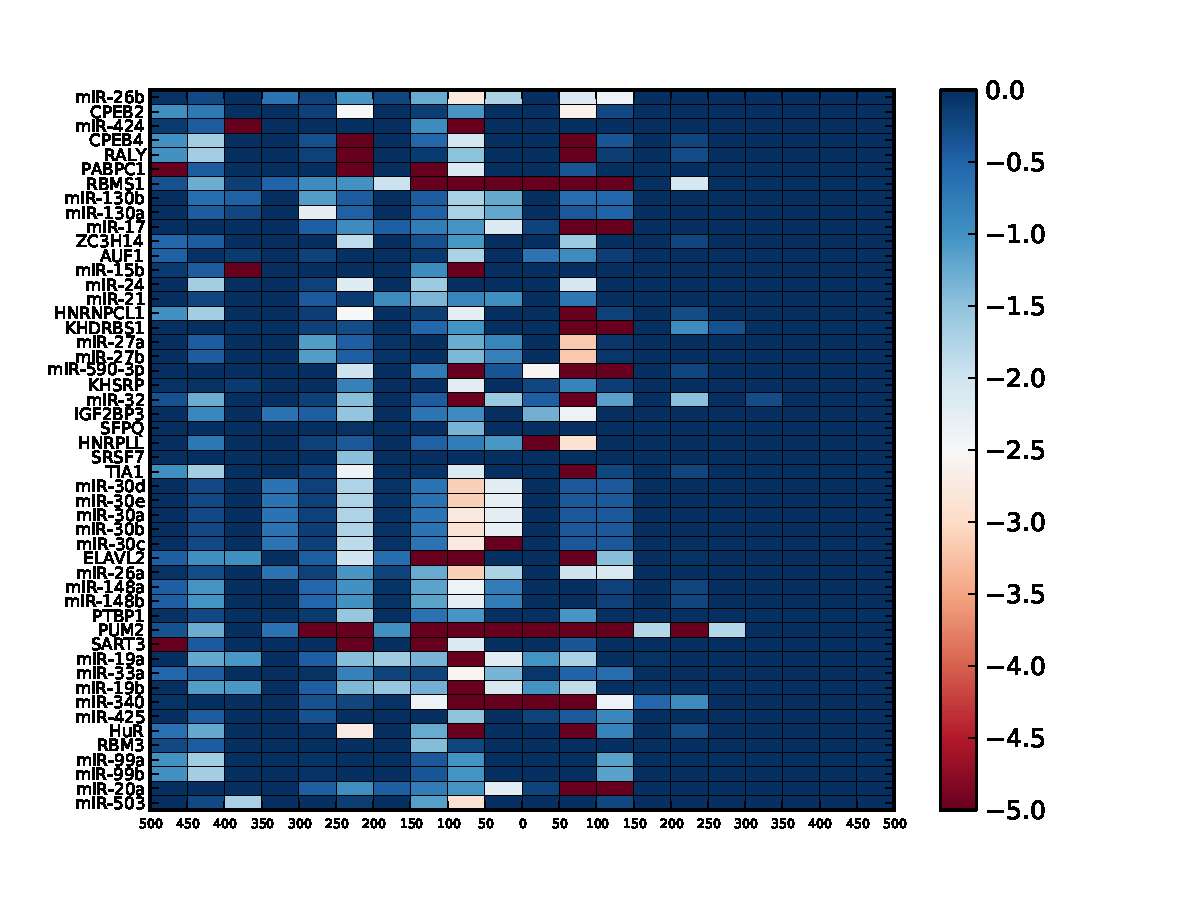
\includegraphics[width=1.15\textwidth,clip]{ch4_results_discussion/figures/PUM1_normal_expressed_heatmap_qvalues0.pdf}
\caption[Interaction of PUM1 protein with its interacting factors]{Q-values of co-occurrence analysis between binding sites of PUM1 and binding sites of its interacting factors (Normal shuffle).}
\label{PUM_qvalue_heatmap}
\end{figure}
%\shorthandon{=}
\clearpage
Figure \ref{PUM_qvalue_heatmap} shows the q-value heatmap of the co-occurrence between PUM1 binding sites and other interacting factors. Each row represents a factor interacting with PUM1 and there are 20 windows in each row (10 windows in upstream and 10 windows in downstream of PUM1 sites, 5o nt long each). Y-axis shows the q-values calculated from impractical P-values. Lower values represent significant number of binding sites of the interacting factor. We observed that some factors, specifically miRNAs, tend to localize near the binding sites of PUM1. PUM1(2) is known to interact with miRNAs and there are several prominent examples of their cooperative interaction, including its collaboration with miR-221/222 to repress the expression of their target p27 gene. We suppose that they are similar interactions between PUM1(2) and miRNAs. We aim to investigate this phenomenon in detail. First, we determined miRNAs interacting with PUM1(2), considering q-values from previous co-occurrence analysis. Next, we assess the effect of their interaction on mRNA half-life measurement in HEK293 cells (Schueler dataset, \cite{schueler_14}). We classified the transcripts into five groups: (i) those that do not have any PUM1(2) or miRNA sites (-PUM -miRNA); (ii) those that contain at least one CLIP-supported PUM1(2) site but do not contain any site of an interacting miRNA (+PUM -miRNA); (iii) those that contain at least one interacting miRNA site but do not contain any PUM1(2) sites (-PUM +miRNA); (iv) those that contain at least one CLIP-supported PUM1(2) site and at least one site of an interacting miRNA (+PUM +miRNA (not stem-loop)); and (v) a subset of the transcripts in group (iv) where there exists at least one pair of PUM1(2)-miRNA site that forms a stem-loop (+PUM +miRNA (stemloop)).

%\shorthandoff{=}
\begin{figure}[H]
	\centering
	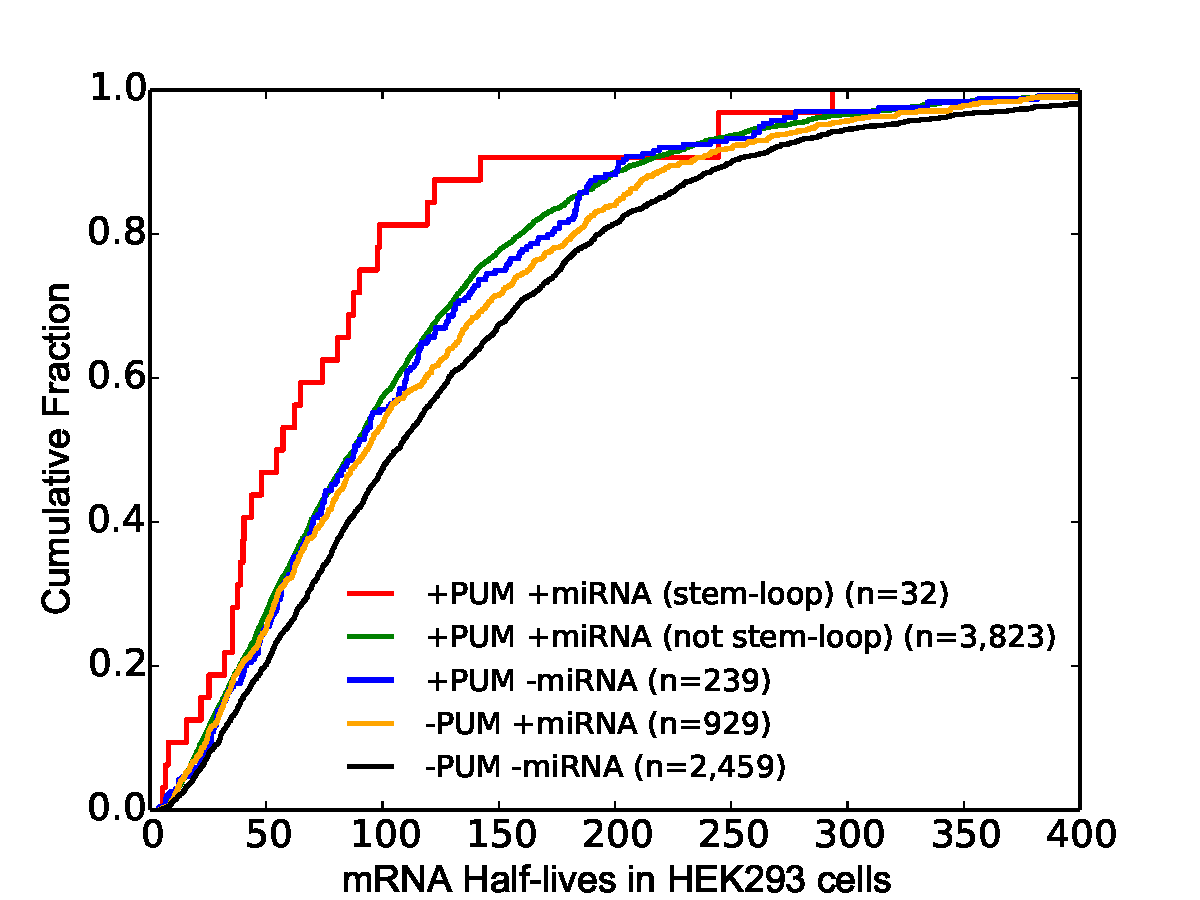
\includegraphics[width=0.7\textwidth,clip]{ch4_results_discussion/figures/Figure6}

\caption[Effect of co-occurrence of PUM1(2) and miRNA sites to mRNA half-life]{Effect of co-occurrence of PUM1(2) and miRNA sites to mRNA half-life. Transcripts where PUM1(2) and miRNA sites are predicted to be in cooperation with each other (+PUM +miRNA (stem-loop)) have significantly shorter half-lives compared to other transcripts.}
\label{PUM_revcomp}
\end{figure}
%\shorthandon{=}

Figure \ref{PUM_revcomp} shows the comparison of the distribution of half-lives for these five groups. We observed that transcripts in +PUM +miRNA (stem-loop) group have significantly shorter half-lives compared to those in +PUM +miRNA (not stemloop) group (P-value = $0.0061$), +PUM -miRNA group (P-value = $0.0126$) and -PUM +miRNA group (P-value = $0.005$). Also, the difference between the half-lives of the groups +PUM -miRNA and +PUM +miRNA (not stem-loop) is not significant (P-value = $0.52$) pointing out that the functional effect of co-occurrence of PUM1(2) and interacting miRNAs is only seen when they form a stem-loop. This observation suggests that the cooperation between PUM1(2) and miRNAs is a widespread phenomenon.

As figure \ref{PUM_qvalue_heatmap} shows, PUM1(2) and miRNA binding sites are tend to be close to each other. It increases the chance to form stem-loops and therefore increases the possibility of collaboration interaction between these factors. As such, it leads to faster degradation of transcript half-lives. We plotted similar heatmaps for each factor, considering all three shuffle types. Appendix \ref{chp:appendixB} contains a selected number of those heatmaps.

\section{Analyzing preferences of PUM binding sites}

\subsection{PUM1(2) tends to bind to the 3'-end of its target mRNAs}

As a follow-up, we investigated the q-values from previous analysis and interestingly noticed that windows in the downstream of PUM1 binding sites are not significant for almost all interacting factors. It also holds true for PUM2, considering all three shuffle types. One possible explanation for this issue is that PUM1(2) tends to bind to the end of transcripts. As a result of that, they are no or little amount of other binding sites in the downstream of PUM1(2) sites. In order to further prove our hypothesis, we divided each transcript containing PUM1(2) into ten equal windows and counted the number of PUM1(2) in each window. Next, we added them up to get the total amount of binding sites in each window. We observed that windows in the downstream of the transcripts contain higher amount of PUM1(2) binding sites compared to other windows. This phenomenon is also accordance with a similar finding in Jiang et al. \cite{jiang_13}.

\subsection{Effect of number of binding sites of PUM1(2) and its interacting miRNAs on stability of transcripts}

We already determined that some factors might interact with PUM1(2). MiRNAs decrease expression of their target transcripts and as we mentioned in previous section, some of these miRNAs are likely to interact with PUM1(2) to effect stability of their target mRNAs. In this analysis we aim to investigate the effect of such interactions on stability of transcripts. 

In the co-occurrence analysis, we determined interacting factors for each factor of interest. Here we only consider miRNAs among interacting factors of PUM1(2) because their effect on transcripts are similar. Besides, we suppose that these interacting factors should be in certain distance to get involved in a cooperative interaction. Therefore, we define interacting miRNAs by only considering factors in 200 nt range of each PUM1(2) protein. We grouped transcripts in case of their PUM1(2) and interacting miRNA sites count and then compared them using the mRNA half-life measurement in HEK293 cells. We classified transcripts as follows: (i) those that have no PUM1(2) site at all. (ii) those transcript which contain at least two up to five sites. {iii} those transcripts which contain more than five sites.

%\shorthandoff{=}
\begin{figure}[H]
	\centering
	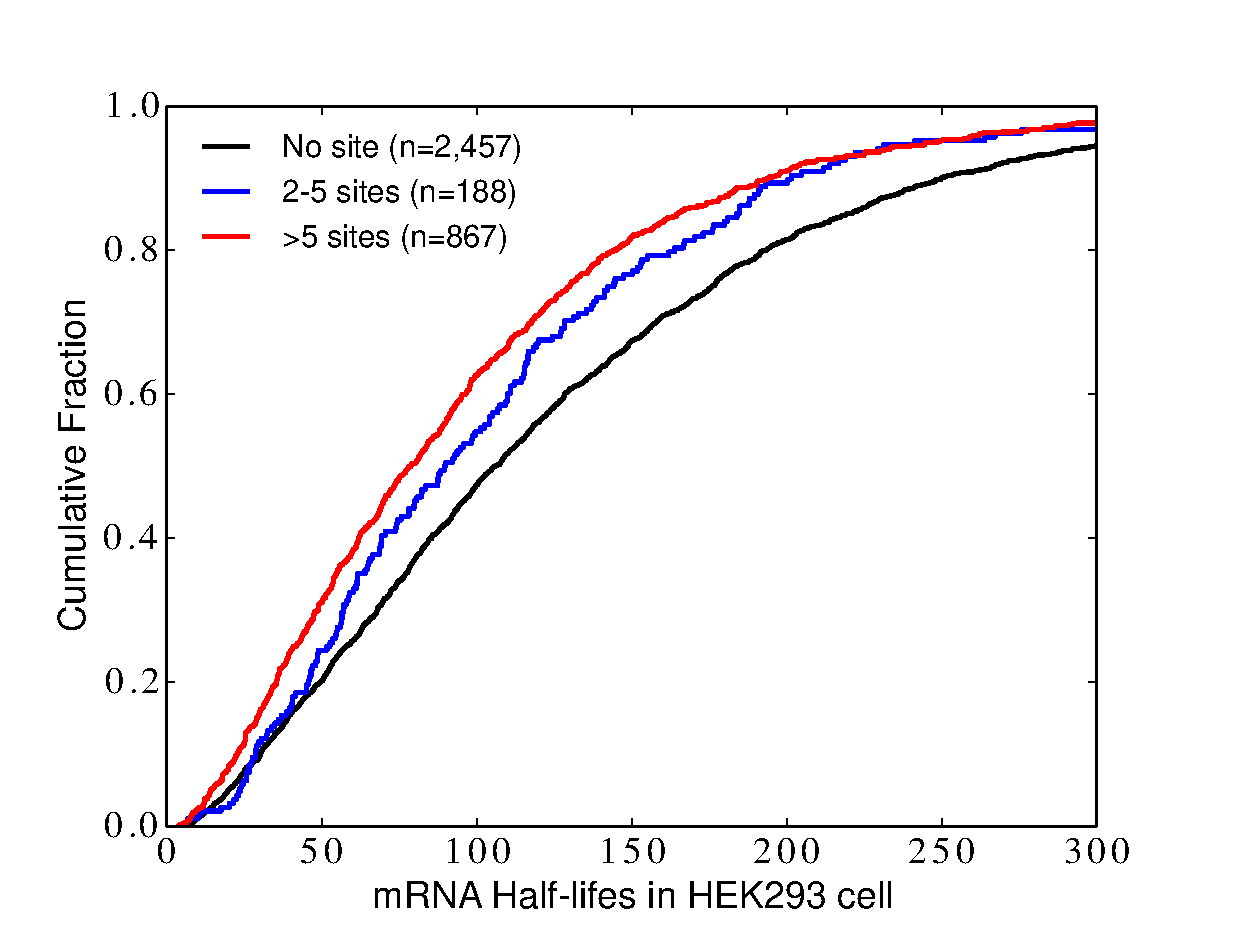
\includegraphics[width=0.7\textwidth,clip]{ch4_results_discussion/figures/pum_plus_intmiRNAs_number_of_sites}

\caption[Effect of binding sites of PUM1(2) and its interacting miRNAs count on expression of transcripts]{Functional effect of number of PUM1(2) and its interacting miRNA sites on transcripts. Transcripts with more binding sites of PUM1(2) and its interacting miRNAs have significantly shorter half-lives compared to other transcripts.}
\label{PUM_number_of_sites}
\end{figure}
%\shorthandon{=}

Figure \ref{PUM_number_of_sites} shows the differences between these groups. We observe that transcripts in group three have shorter half-lives compared to those transcripts with two up to five sites and also those with no PUM1(2) sites at all (P-values = $0.03$ and $7.91E-20$ respectively). This analysis demonstrates that the more PUM1(2) and its interacting miRNAs sites exist in a transcript, the higher possibility there is that it will downregulate faster.

\subsection{The effect of distance between binding sites of PUM1(2) on stability of mRNAs}

It is also clear from the figure \ref{PUM_qvalue_heatmap} that PUM1 binding sites are close to each other. Q-values are significant in 150nt up and down stream of the PUM1 binding sites when we consider its own sites as interacting factors. We suppose that this is because PUM1(2) interacts with itself. In order to further investigate this issue, we analyzed the effect of number of PUM1(2) binding sites on transcripts stability. Also we assessed the difference between two conditions in which PUM1(2) binding sites co-occur in close ranges whereas they are not close to each other.

In order to investigate our hypothesis, first we need to classify sites as \textit{close} and \textit{not close} to each other. We determined two sites as \textit{close} to each other when there was at most 50 nucleotides between the starting position of those sites, otherwise we considered them as \textit{not close}. The reason for considering this threshold is that we are trying to focus on those PUM1(2) sites which are inside same stem loop otherwise they will be unlikely to cooperate with each other. We classified transcripts into three groups: (i) those that do not contain any PUM1(2) sites. (ii) those that contain two or more PUM1(2) sites and there is at least two sites which are close to each other. (iii) those that contain two or more PUM1(2) sites but none of them are close to each other. Figure \ref{pum_close_not_close} shows the mRNA half-life measurement in HEK293 cells for these three groups. We observe that transcripts with more than two sites (close) have significantly shorter half-lives compared to those with more than two sites but with no close sites (not close) (P-value = $2.98E-05$). Besides, both first and second groups have significantly shorter half-lives compared to the transcripts with no PUM1(2) sites at all (P-values = $1.04E-22$ and $2.6E-04$ respectively). This observation represents that transcripts with close PUM1(2) sites tend to have shorter half-lives and the reason for this is likely because PUM1(2) binding sites are cooperatively interacting with each other.

%\shorthandoff{=}
\begin{figure}[H]
	\centering
	\subfloat[]{
	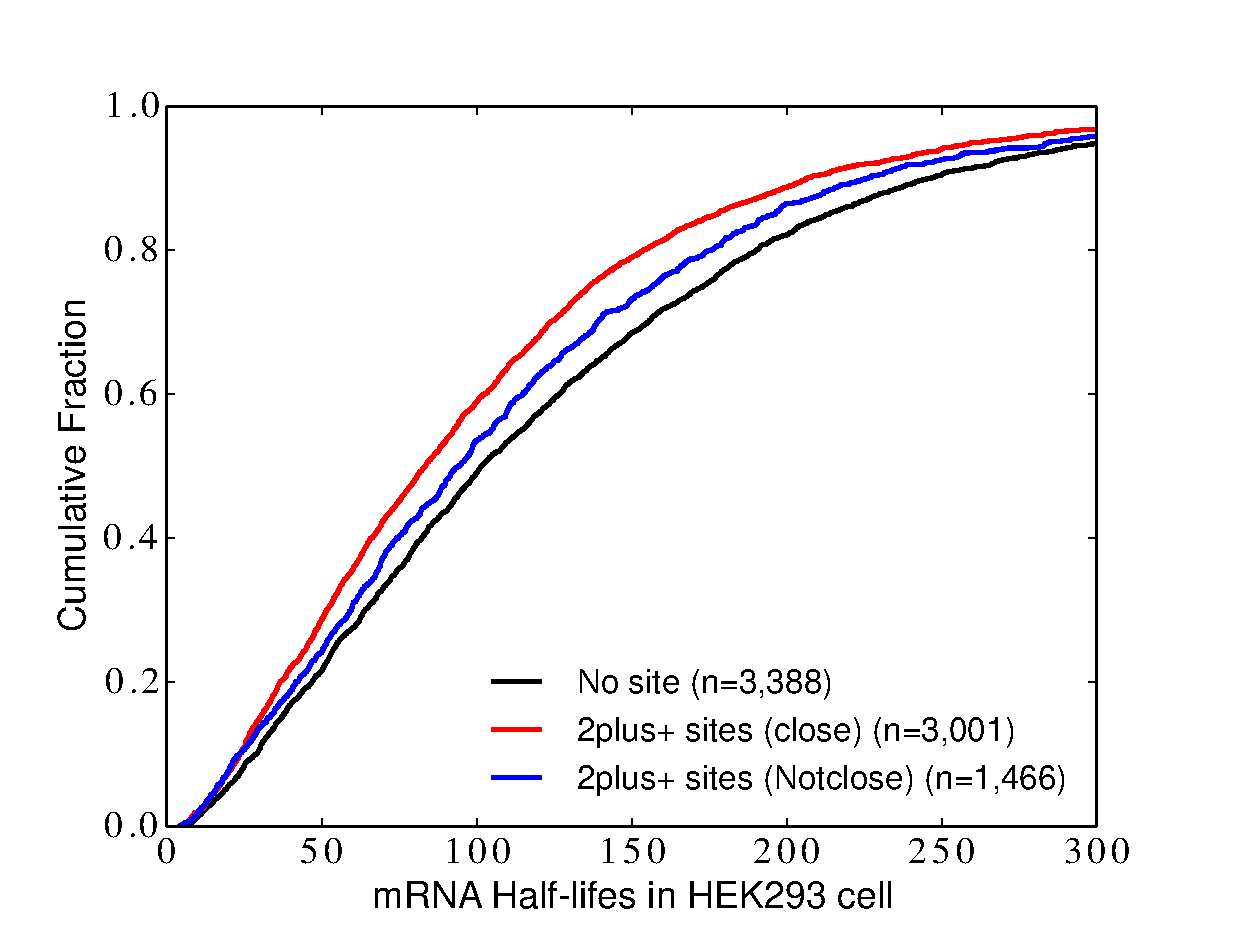
\includegraphics[width=0.9\textwidth,clip]{ch4_results_discussion/figures/pum_close_notclose}
    \label{pum_close_not_close}
}
\caption[Effect of close and not close PUM binding sites on expression of transcripts]{Functional effect of close PUM1(2) sites on stability of mRNAs. Transcripts where PUM1(2) binding sites are close to each other have significantly shorter half-lives compared to other transcripts where there are no close PUM1(2) sites.}
\end{figure}
%\shorthandon{=}

Although the result for this analysis shows that transcripts with close PUM1(2) sites are destabilizing faster than those with no close PUM1(2) sites at all. However, the disadvantage of this analysis is that we ignore the fact that this difference may be not clearly because of interaction between close PUM1(2) sites. Actually when we compare the transcripts in first and second groups, we are not clearly sure that the difference is due to the phenomenon of close sites. It might be related to the number of PUM1(2) sites. One solution is to restrict the number of PUM sites and then re-plot the figure but it leads to data loss and weakens the output. Another solution is to distinguish the results according to number of close sites. However, this time we should make number of sites restrict. Actually, there are two variables here, number of sites and number of close sites. In order to get a better result, we should take these two variables in to consideration at the same time. However, this approach reduces the transcripts count and makes the result not reliable. In the future, we may reintroduce this analysis for larger group of transcripts to get much more reliable result.

\clearpage
\section{Predicting stability and gene expression with a logistic regression model}

In this analysis, we took into account the effect of multiple factors to predict stability and gene expression levels. Figure \ref{zhao_nostr_nogparclip} compares the AU-ROC curves of three models that predict half-life or steady-state mRNA abundance in Zhao dataset: (i) \textit{miRNAs}, \textit{activators} and \textit{repressors} are used as features (miRNAs + RBPs); (ii) counts of 16 2-mers that represent dinucleotide content are used as features (dinucleotide content); (iii) the combination of features used in model (i) and (ii) are used (dinucleotide content + miRNAs + RBPs). 

%\shorthandoff{=}
\begin{figure}[H]
	\centering
	\subfloat[]{
	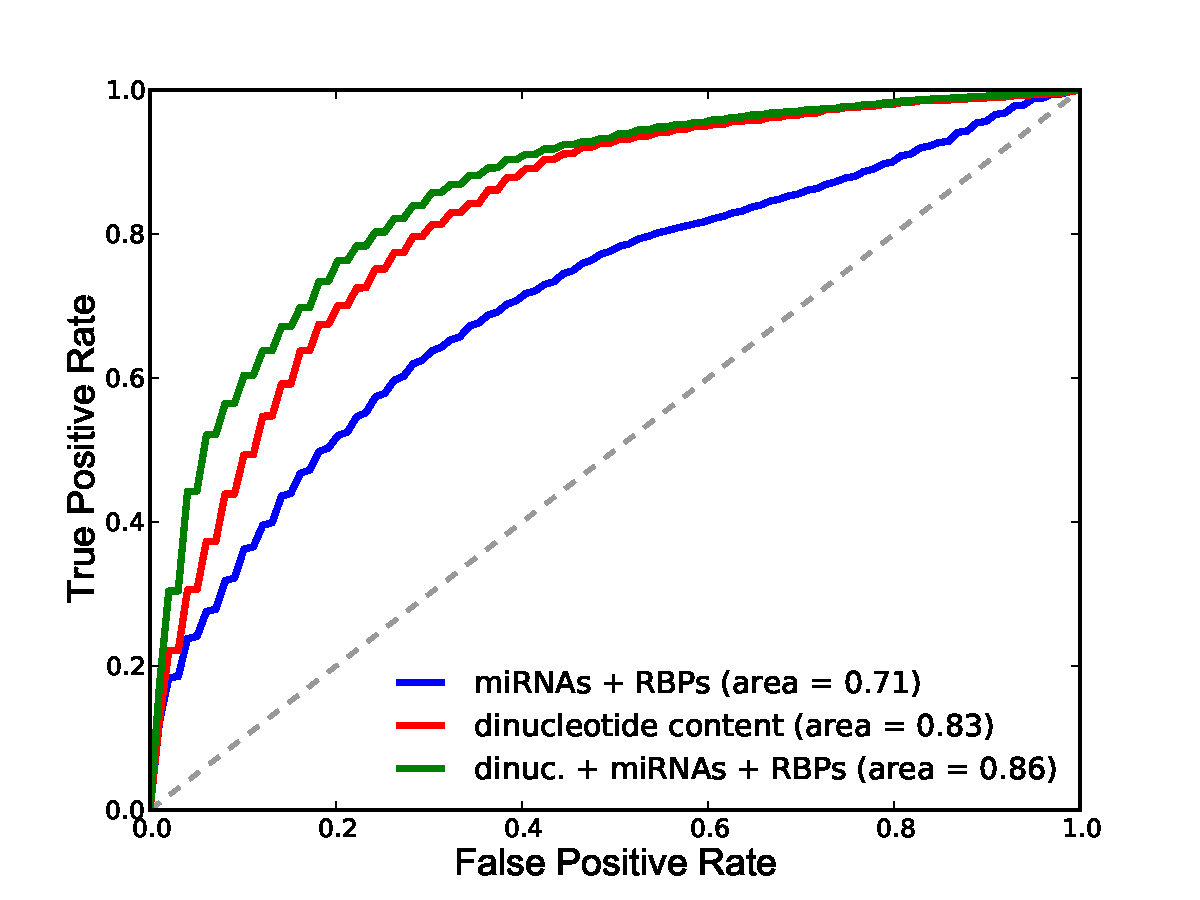
\includegraphics[width=0.6\textwidth,clip]{ch4_results_discussion/figures/Figure7a}
    \label{zhao_halflife_nostr_nogparclip}
}
\quad
	\subfloat[]{
    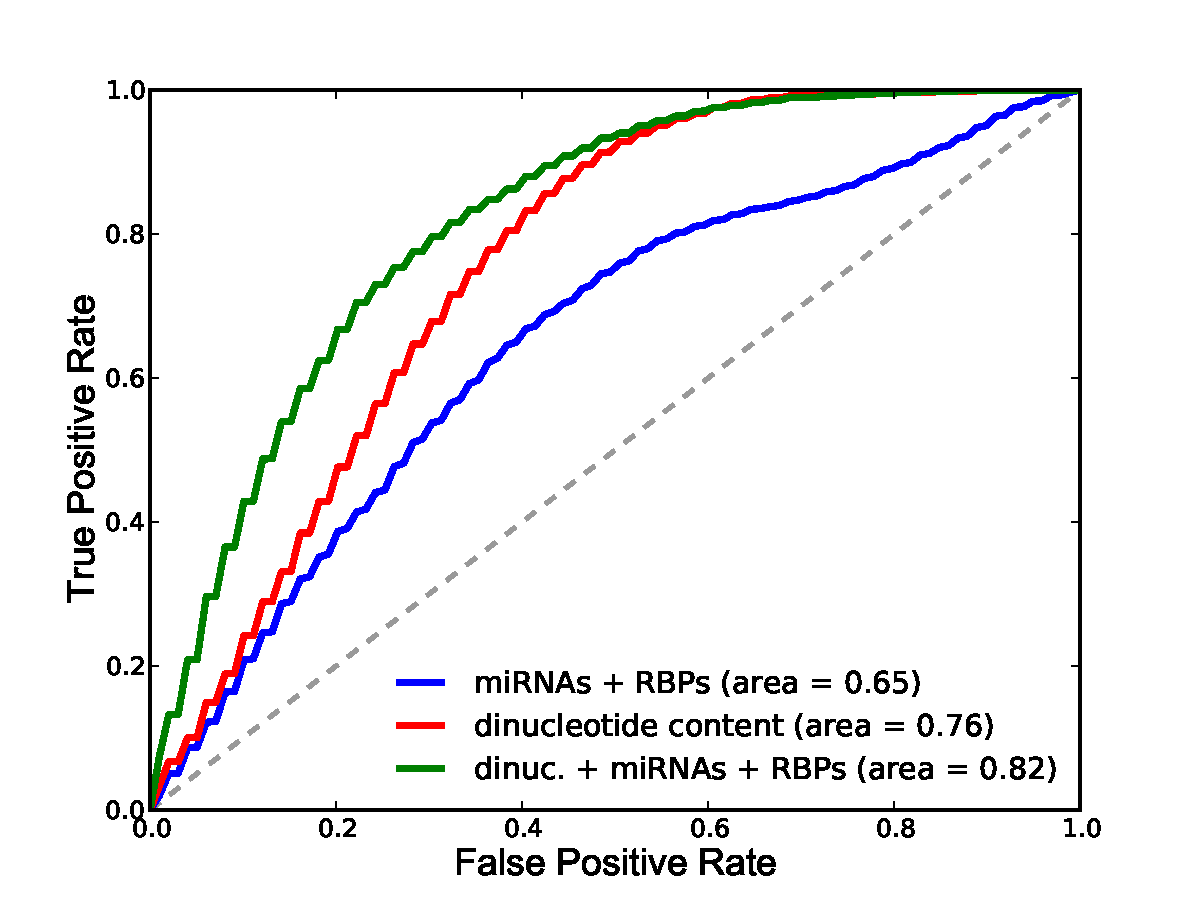
\includegraphics[width=0.6\textwidth,clip]{ch4_results_discussion/figures/Figure7b}
    \label{zhao_steady_nostr_nogparclip}
}

\caption[Predicting stability and gene expression with a logistic regression model]{Results of predicting half-life and steady-state mRNA levels in Zhao dataset.  \subref{zhao_halflife_nostr_nogparclip} ROC curves (interpolation of 100 curves) of models that predict half-life in Zhao dataset, area shows the average of 100 AU-ROC values. \subref{zhao_steady_nostr_nogparclip} ROC curves (interpolation of 100 curves) of models that predict steady state mRNA abundance in Zhao dataset, area shows the average of 100 AU-ROC values. }
\label{zhao_nostr_nogparclip}
\end{figure}
%\shorthandon{=}

We observe that dinucleotide features alone perform much better than features formed from sites of miRNAs and RBPs (Wilcoxon signed-rank test applied to 100 AU-ROCs from two models, P-value = $6.0E-18$ for half-life and P-value = $2.5E-17$ for mRNA abundance); however, the addition of miRNA and RBP features on top of dinucleotide content features improves the predictive power of the model (P-value = $1.1E-17$ for half-life and P-value = $9.1E-18$ for mRNA abundance). %Fitted parameter values can be seen in Supplementary Figure 1.

%\shorthandoff{=}
\begin{figure}[H]
	\centering
	\subfloat[]{
	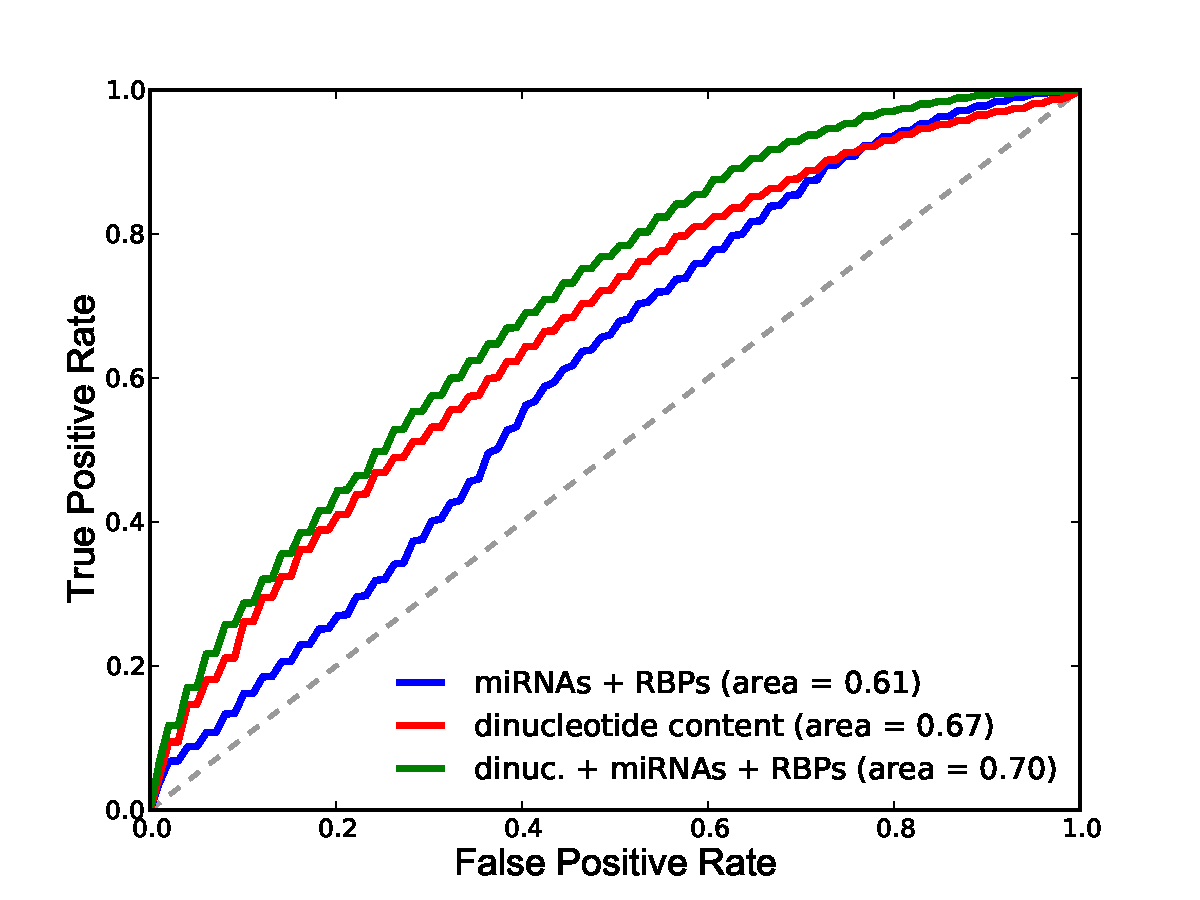
\includegraphics[width=0.65\textwidth,clip]{ch4_results_discussion/figures/Figure8a}
    \label{schueler_halflife_HEK293_500}
}
\quad
	\subfloat[]{
    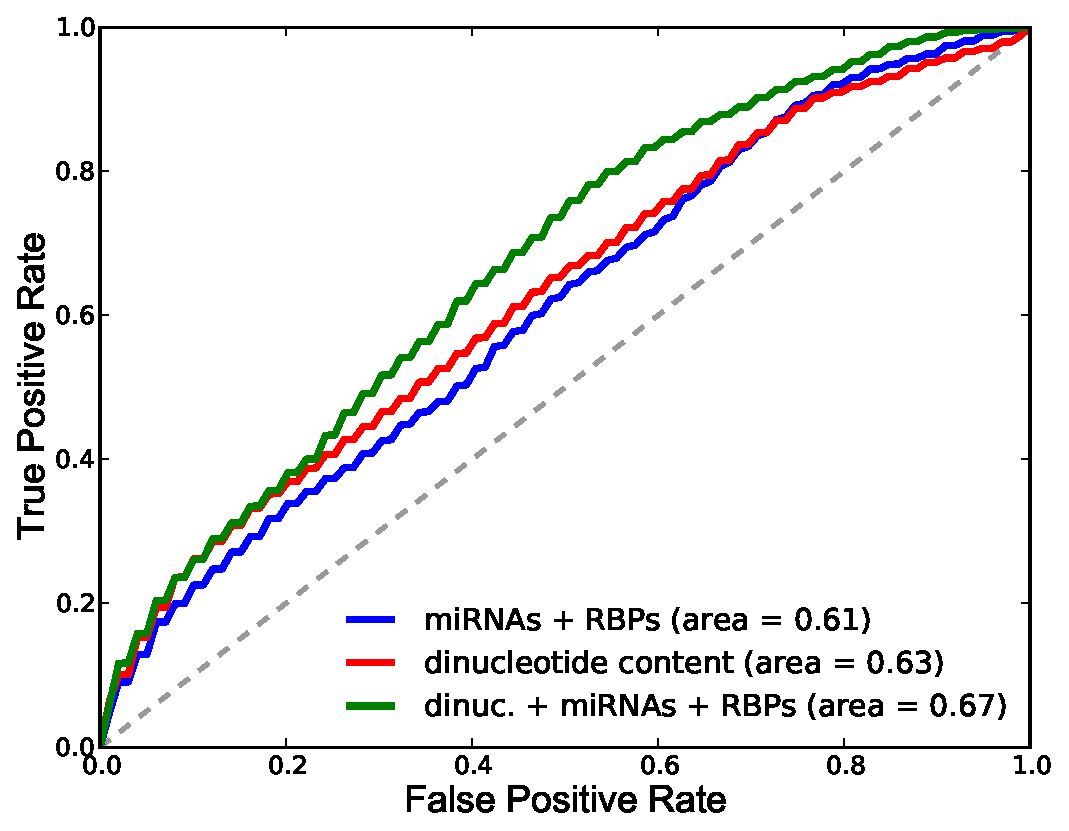
\includegraphics[width=0.65\textwidth,clip]{ch4_results_discussion/figures/Figure8b}
    \label{schueler_halflife_MCF7_500}
}
\caption[Optional caption for list of figures]{Results of predicting half-life in HEK293 and MCF7 cells (Schueler dataset)  \subref{schueler_halflife_HEK293_500}  ROC curves (interpolation of 100 curves) of models that predict half-life in HEK293 cells, area shows the average of 100 AU-ROC values.  \subref{schueler_halflife_MCF7_500} ROC curves (interpolation of 100 curves) of models that predict half-life in MCF7 cells, area shows the average of 100 AU-ROC values.}
\label{Schueler_halflife_nostr_nogparclip}
\end{figure}
%\shorthandon{=}

We repeated the same analysis with half-life datasets in HEK293 and MCF7 cells (Schueler dataset) this time calculating features considering the 3'UTRs of the transcripts. Figure  \ref{schueler_halflife_HEK293_500} and \ref{schueler_halflife_MCF7_500} show the ROC curves of the logistic regression models predicting half-life in HEK293 and MCF7 cells, respectively. For both cell types, the increase in AU-ROC between model(i) and model(ii); and between model(ii) and model(iii) is significant according to Wilcoxon signed-rank test (P-values are $1.9E-12$ and $9.0E-12$ for HEK293 cells and $6.8E-05$ and $2.7E-13$ for MCF7 cells). 

We also checked whether our features simply represent a bias of 3'UTR length. The 3'UTR segments in Zhao dataset are all of the same length whereas the Schueler dataset contains 3'UTRs of variable length. Predicting half-life with only 3'UTR length in HEK293 and MCF7 cells results in a mean AU-ROC value of 0.545 and 0.548, respectively. This confirms that our features do not simply represent 3'UTR length.

In addition to counting simply the number of binding sites as above, we also tried using more advanced features. For instance, we used the sum of the accessibility of sites of \textit{miRNAs}, \textit{activators} or \textit{repressors} as features. We also tried considering only gPARCLIP- or CLIP-supported RBP sites and miRTarBase or Ago2-CLIP supported miRNA sites. Lastly, we took into account the effect of competition by counting the sites that overlap with other factors' sites as 0.5 rather than 1. However, neither of these modifications resulted in improved performance in Zhao or Schueler datasets (data not shown).
% CHAPTER 5
\chapter{CONCLUSION AND FUTURE WORK}
\label{chp:chapter5}

\section{Conclusion}

PTR is mediated by the interactions of RBPs and miRNAs with target sites on mRNAs. Recent studies show that these two major post-transcriptional regulators do not act independently. Indeed, they are involved in competitive or cooperative interactions with each other. In this thesis, we considered the effect of multiple factors concurrently.  First, we mapped all RBP and miRNA binding sites on human 3’UTRs. We took advantage of \textit{in vitro} (RNAcompete), \textit{in vivo} (CLIP, gPARCLIP) and computational methods (TargetScan, PicTar) in order to identify and predict binding sites of RBPs and miRNAs. We also considered the secondary structure of 3’UTRs by predicting with computational methods RNAplfold and Sfold.   

First, we compared CLIP-supported sites and other sites in terms of accessibility and conservation. We repeated this analysis considering CLIP-supported sites of PUM2, HuR, IGF2BP1-3, and QKI RBPs. We observed that CLIP-supported sites of these RBPs are more conserved compared to other sites. In case of accessibility, we observed that CLIP-supported sites of HuR are more accessible which is in line with previous studies \cite{hur_accessibility, kazan_10}. It also holds true for CLIP-supported sites of QKI. However, in contrast to what we expected, CLIP-supported sites of PUM2 are less accessible. Besides, CLIP-supported sites of IGF2BP1-3 are also less accessible compared to other sites.

Next, we utilized the HuR knockdown dataset and checked whether CLIP-supported sites of HuR show any difference compared to other sites in terms of functional outcome upon HuR depletion. Indeed, we observed that transcripts with CLIP-supported HuR sites are destabilized more compared to transcripts with no CLIP-supported sites at all. We also identified HuR sites that overlap with binding sites of other factors and considered them as being in competition. Next, we investigated the effect of competition to HuR function. We observed that transcripts in which all HuR sites were in competition with other factors show less change upon HuR knockdown. 

In order to find potential interacting factors, for each pair of factors, we checked whether their binding sites co-occur more often than expected by random chance. We observed that binding sites of miRNAs tend to occur near PUM2 sites. In order to investigate the possible interaction between these factors, we classified transcripts into two groups: first, those transcripts that contain a site of PUM2 and a site of one of its interacting miRNAs in a stem-loop. Second, those transcripts that still contain sites of both of these factors but not in a stem-loop. We observed that transcripts in the first group have shorter half-lives compared to the second one.

Besides, we observed that there are no or little amount of interacting factors in the 3’-end of binding sites of PUM1(2). We think that it is because PUM1(2) tends to bind to the 3’-end of transcripts.  We divided the transcripts which contain binding sites of PUM1(2) into several windows and counted the number of binding sites in each of them. As expected, we observed that the nearest window to the 3'-end of transcripts contains the most binding sites of PUM1(2). Furthermore, we assessed the effect of number of PUM1(2) binding sites on mRNA stability and observed that transcripts with more PUM1(2) binding sites tend to have shorter half-lives. Besides, we observed that binding sites of PUM1(2) tend to col-localize near each other. We supposed that in such conditions, PUM1(2) may interact with itself. We classified the transcripts into two groups: (i) Transcripts which contain binding sites of PUM1(2) with at least two sites close to each other. (ii) Transcripts which contain PUM1(2) sites but there are no binding sites close to each other. We observed that transcripts in the first group have shorter half-lives. This indicates that binding sites of PUM1(2) may involve in interaction with each other which may lead to faster degradation of their target mRNA.

Finally, we trained a logistic regression with features compiled from counts of sites of miRNAs, RBPs and dinucleotides to predict half-life and mRNA abundance. The high performance of the dinucleotide-only model is in line with 2013 DREAM5 challenge results where motif models that consider dinucleotide content perform well \cite{weirauch_13}. We hypothesize that dinucleotide features capture the binding motifs of RBPs or miRNAs. However, we observed that including counts of RBP and miRNAs sites improves the performance, and we achieved a 10-fold CV AU-ROC of 0.86 in predicting half-life in BEAS-2B cells. We also considered alternative ways to compile the features: (i) counting RBP sites that are only gPARCLIP or CLIP-supported; (ii) summing the accessibility of sites; and (iii) considering the competition between the factors. However, these modifications did not increase the predictive performance. The first modification may not have improved performance as only 7 out of 19 RBPs that are in activators and repressors group have CLIP data. Also, counting sites with gPARCLIP support may not result in an accurate estimate of the activity of a specific RBP as the identity of the bound RBP in a gPARCLIP-determined peak is unknown. Lastly, gPARCLIP and most CLIP experiments have been performed in HEK293 cells, whereas we predict half-life and transcript abundance in other cell types such as BEAS-2B and MCF7 cells. The second modification where we considered the accessibility of sites might result in a better performance as our knowledge of mRNA secondary structure gets more accurate. Another issue related to this modification could be our assumption that all RBPs and miRNAs prefer binding to accessible regions. In reality, most of the RBPs have unknown secondary structure preferences and increased knowledge on this would be instrumental.

\section{Future directions}

Despite recent efforts in identifying cooperative and competitive interactions between RBPs and miRNAs, a number of challenges remain in modeling the interaction between these PTR factors. Here we mention some of them which can be handled in the future.

In this thesis, we limited most of our analysis to RBPs HuR and PUM1(2). That’s because they are well-characterized and their effect on mRNA stability is known. With the recent advances in this field, more effect of factors becomes known to scientists. As a future work, we can investigate competitive and cooperative interactions between wider range of factors.

Furthermore, there are also limited datasets that measure genome-wide effect of factors upon their depletion or transfection. We used HuR knockdown dataset to investigate the effect of competition to HuR function. Although we repeated this analysis using for example QKI knockdown dataset, but as the effect of QKI on mRNA stability is not very well known, we cannot reason based on them. In the future, we can repeat our analyses using knockdown or transfection dataset of other RBPs.

Experimental techniques can query mRNA secondary structure \textit{in vivo} \cite{rouskin_14, wan_14}; however, the coverage of the resulting profiles are limited. Recently developed icSHAPE technique \cite{spitale_15} is shown to query the secondary structure of all four bases in mouse ES cells. icSHAPE secondary structure profiles can be utilized in our framework as they become available for human cell types. 
%
% References in Bibtex format goes into below indicated file with .bib extension
\bibliography{referanslar}
\bibliographystyle{unsrt}
% You can use full name of authors, however most likely some of the Bibtex entries you will find, will use abbreviated first names
% If you don't want to correct each of them by hand, you can use abbreviated style for all of the references
\appendix
\chapter{List of RBPs and miRNAs}
\label{chp:appendixA}

\begin{table}[H]
\centering
\caption{List of RBPs and miRNAs for which we performed the co-occurrence analysis}
\begin{tabular}{| c | c |}
\hline
RBPs & miRNAs \\ [0.5ex]
\hline\hline
PUM1 & let-7b \\
PUM2 & miR-1 \\
IGF2BP2 & miR-7 \\
IGF2BP3 & miR-9 \\
HuR & miR-15a \\
HNRNPL & miR-16 \\
QKI & miR-34a \\
LIN28A &  miR-106b \\
ZFP36 & miR-122a \\
PTBP1 & miR-124 \\
 & miR-128a \\
 & miR-132 \\
 & miR-133a \\
 & miR-142 \\
 & miR-148b \\
 & miR-155 \\
 & miR-181 \\
 & miR-181a \\
 & miR-195 \\
 & miR-373 \\
\hline
\end{tabular}
\label{tbl:list_rbp_mirna}
\end{table}
\chapter{Co-occurrence heatmaps}
\label{chp:appendixB}

\section{Co-occurrence q-value heatmap plots of RBPs of interest}

\clearpage
%\shorthandoff{=}
\begin{figure}
   	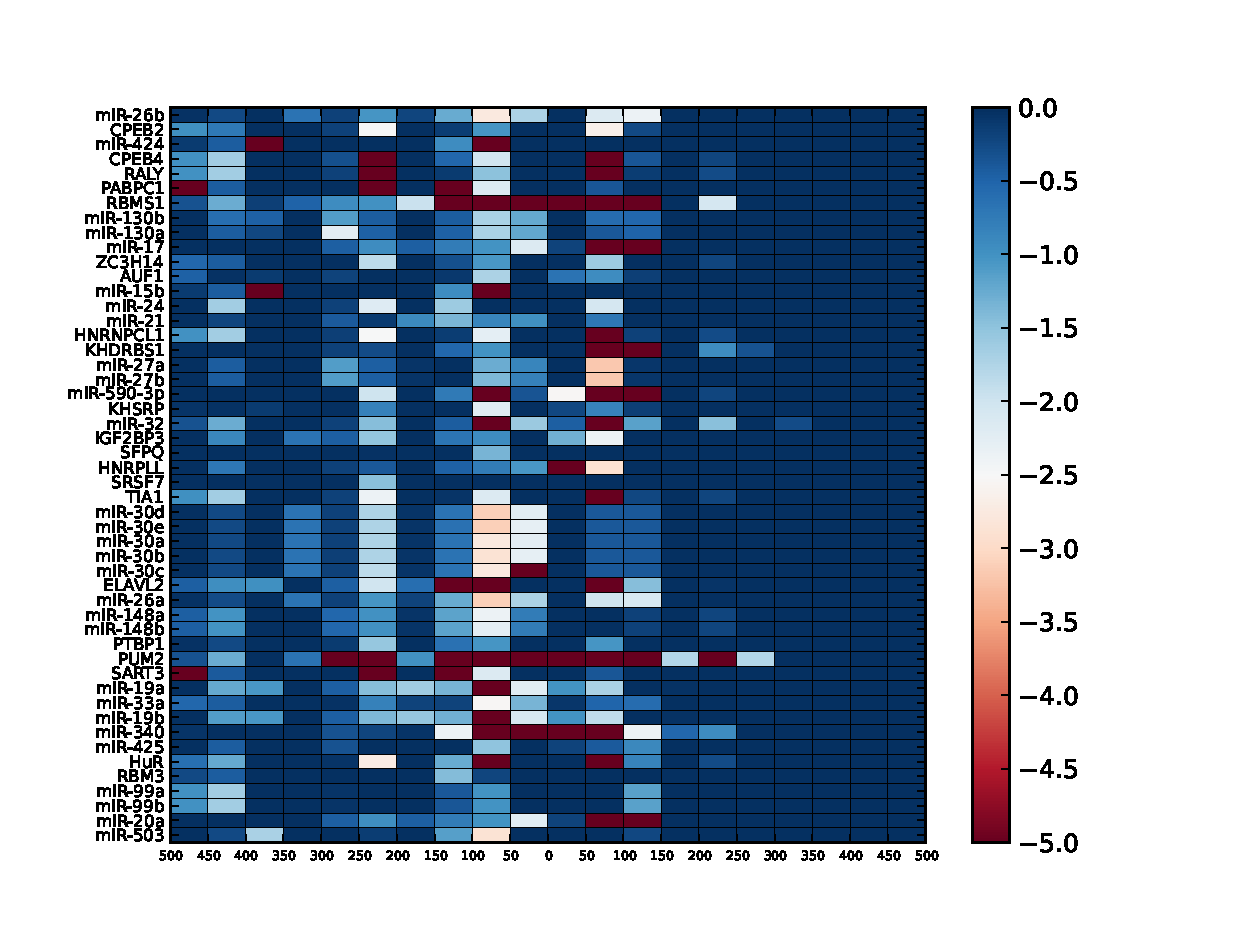
\includegraphics[width=0.9\textwidth]{appendix1/figures/PUM1_normal_expressed_heatmap_qvalues0.eps}
   	\caption{Co-occurrence q-value heatmap plots of binding sites of PUM1 - normal shuffle}
\end{figure}

\begin{figure}
   	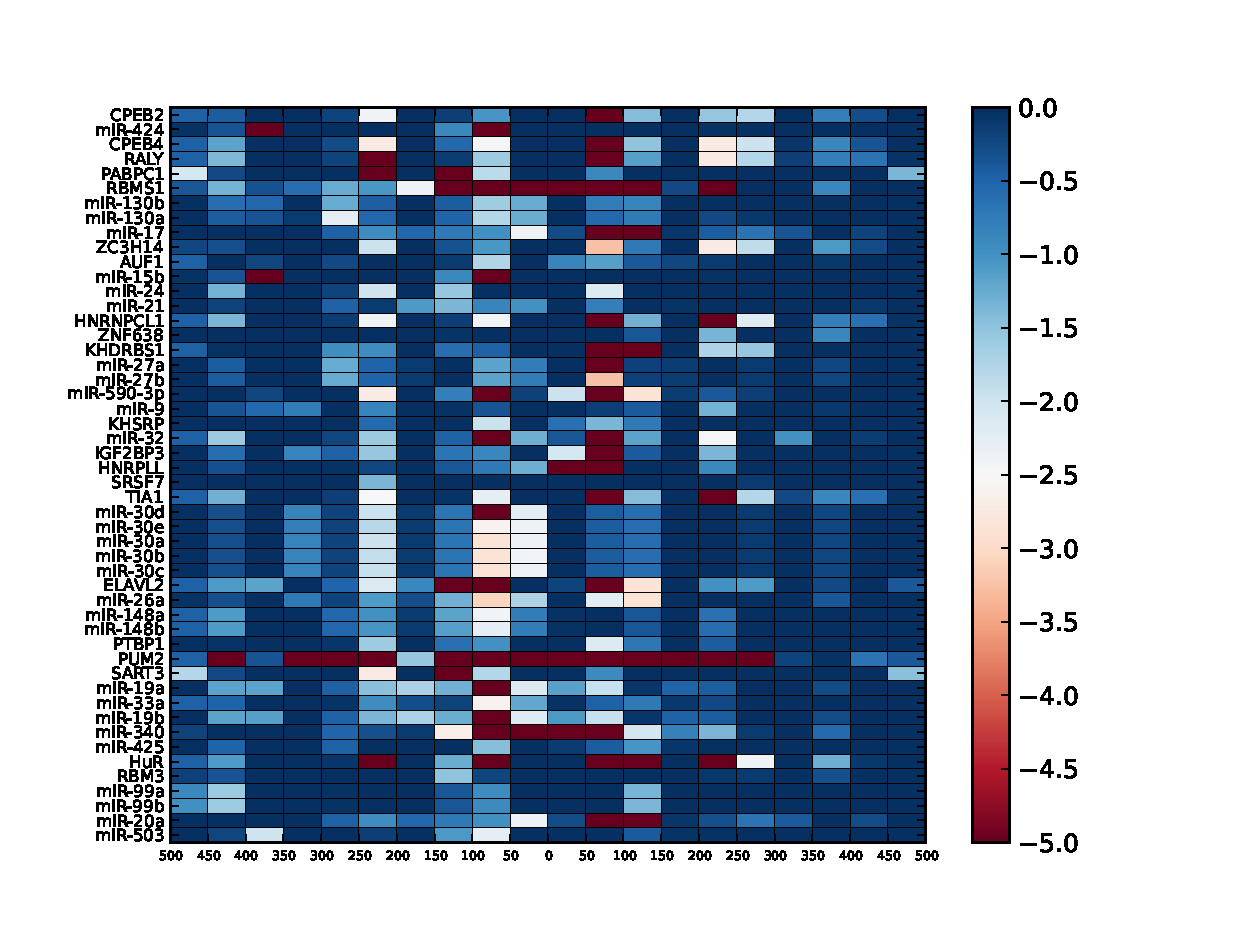
\includegraphics[width=0.9\textwidth]{appendix1/figures/PUM1_decile_expressed_heatmap_qvalues0.eps}
   	\caption{Co-occurrence q-value heatmap plots of binding sites of PUM1 - decile shuffle}
\end{figure}
\clearpage
\begin{figure}
   	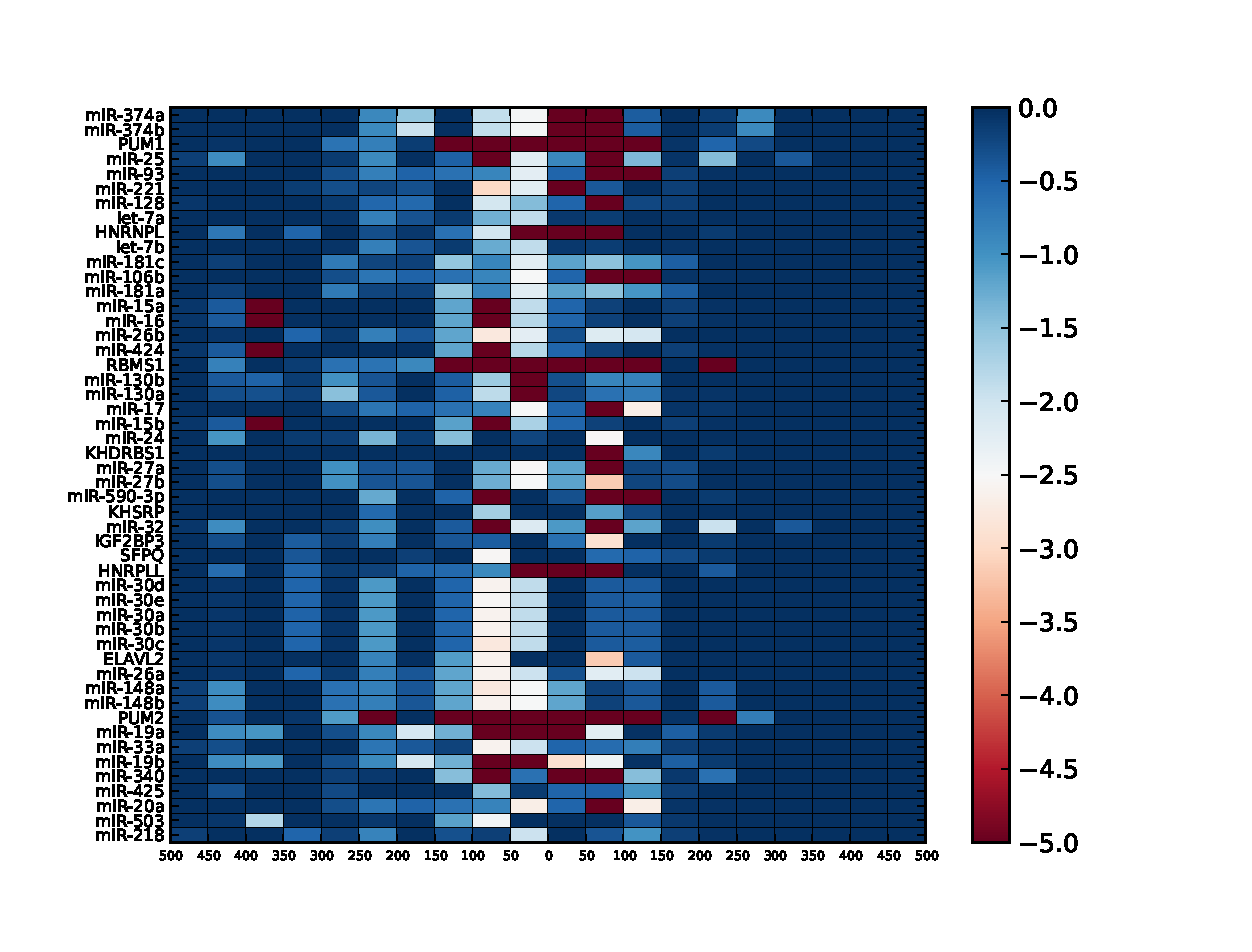
\includegraphics[width=0.9\textwidth]{appendix1/figures/PUM1_AUcontent_expressed_heatmap_qvalues0.eps}
   	\caption{Co-occurrence q-value heatmap plots of binding sites of PUM1 - AUcontent shuffle}
\end{figure}

\begin{figure}
   	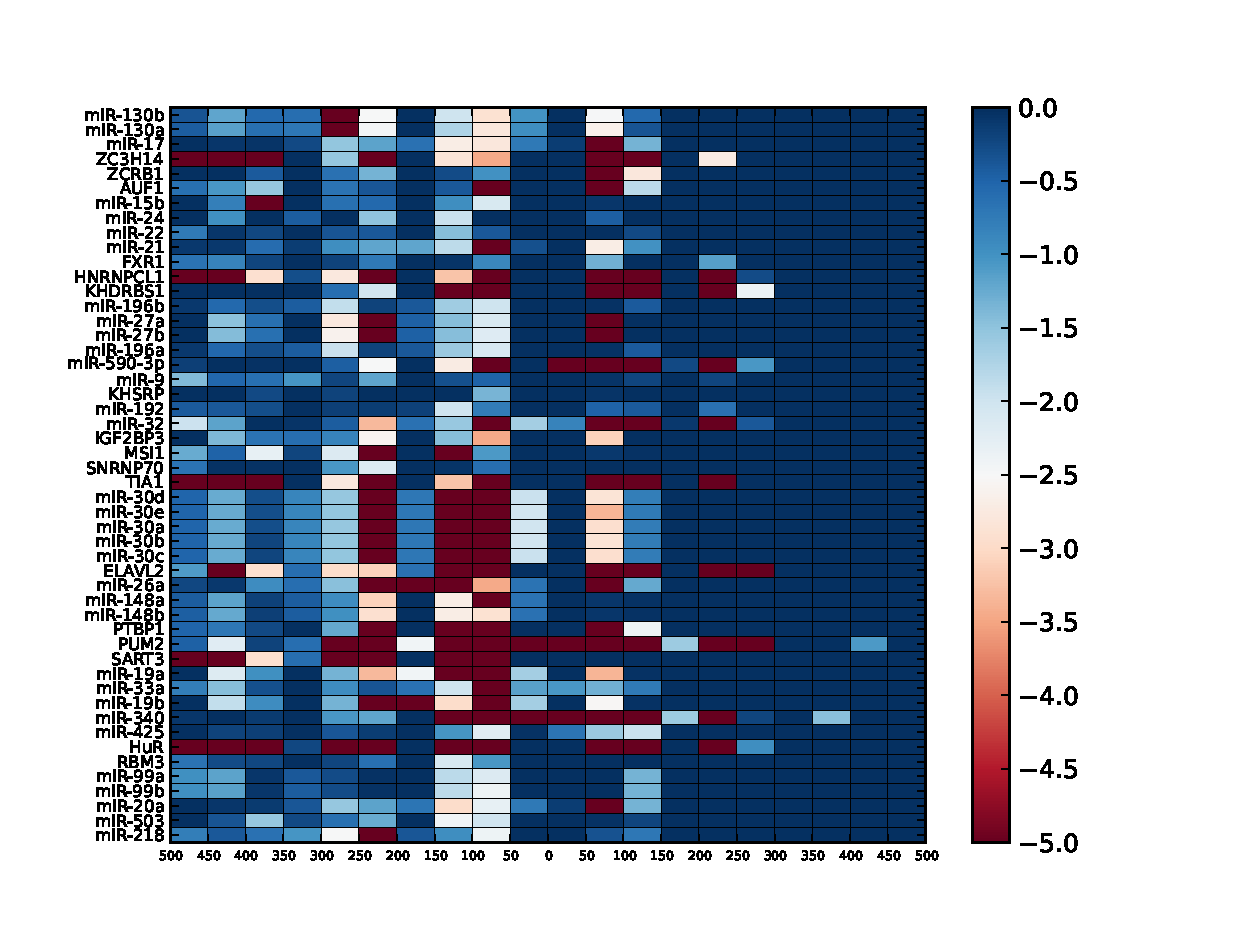
\includegraphics[width=0.9\textwidth]{appendix1/figures/PUM2_normal_expressed_heatmap_qvalues0.eps}
   	\caption{Co-occurrence q-value heatmap plots of binding sites of PUM2 - normal shuffle (Part 1)}
\end{figure}
\clearpage
\begin{figure}
   	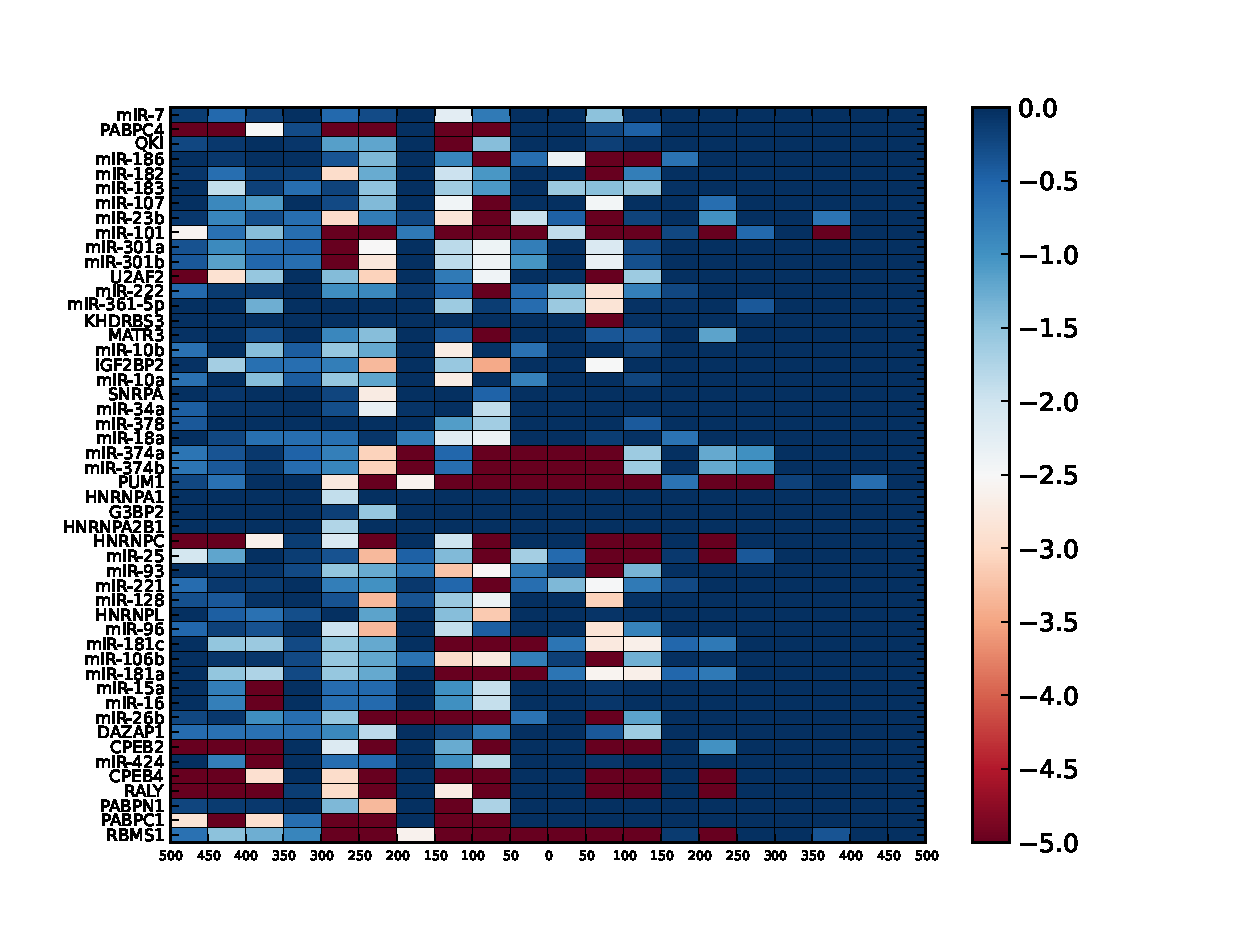
\includegraphics[width=0.9\textwidth]{appendix1/figures/PUM2_normal_expressed_heatmap_qvalues1.eps}
   	\caption{Co-occurrence q-value heatmap plots of binding sites of PUM2 - normal shuffle (Part 2)}
\end{figure}

\begin{figure}
   	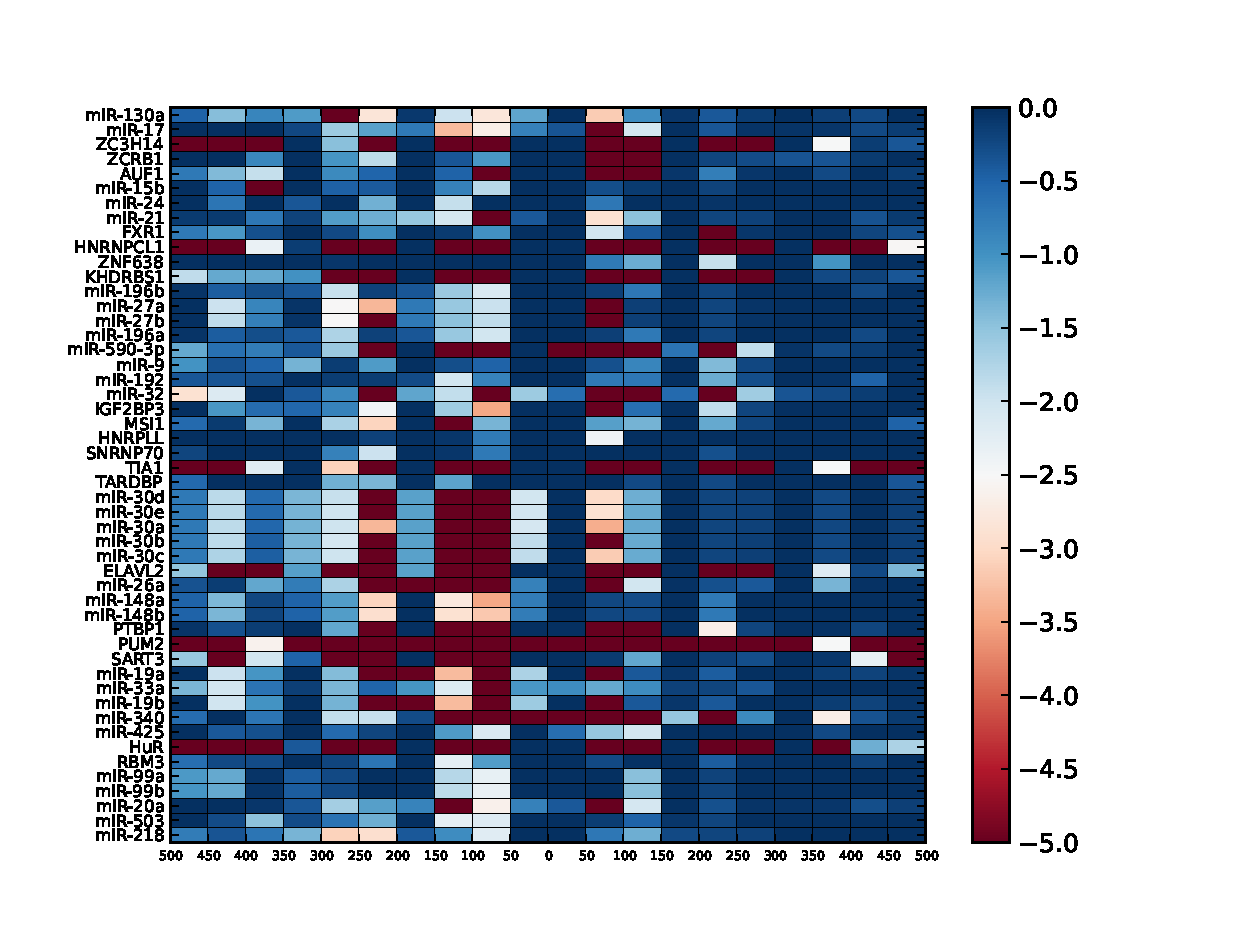
\includegraphics[width=0.9\textwidth]{appendix1/figures/PUM2_decile_expressed_heatmap_qvalues0.eps}
   	\caption{Co-occurrence q-value heatmap plots of binding sites of PUM2 - decile shuffle (Part 1)}
\end{figure}
\clearpage
\begin{figure}
   	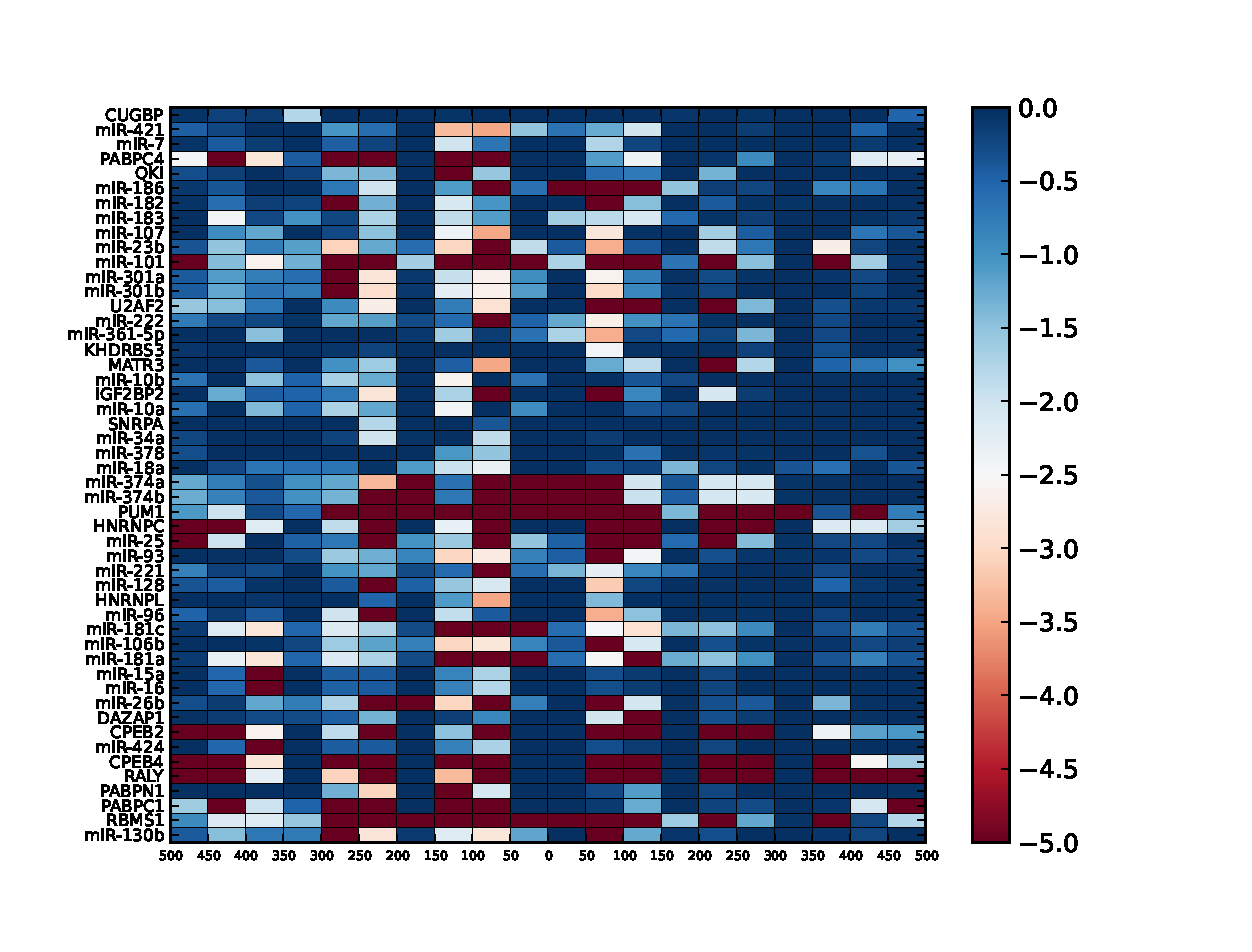
\includegraphics[width=0.9\textwidth]{appendix1/figures/PUM2_decile_expressed_heatmap_qvalues1.eps}
   	\caption{Co-occurrence q-value heatmap plots of binding sites of PUM2 - decile shuffle (Part 2)}
\end{figure}

\begin{figure}
   	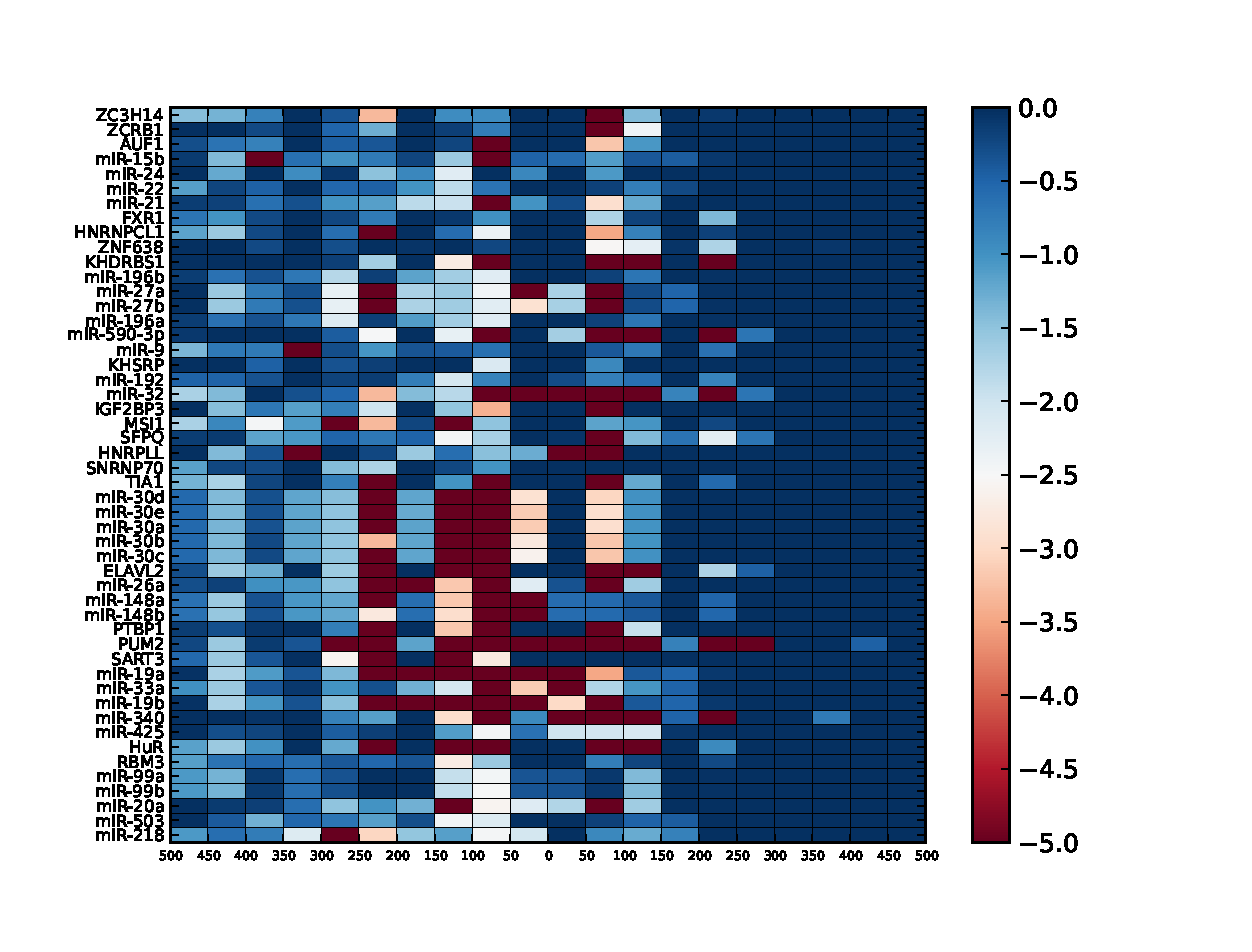
\includegraphics[width=0.9\textwidth]{appendix1/figures/PUM2_AUcontent_expressed_heatmap_qvalues0.eps}
   	\caption{Co-occurrence q-value heatmap plots of binding sites of PUM2 - AUcontent shuffle (Part 1)}
\end{figure}
\clearpage
\begin{figure}
   	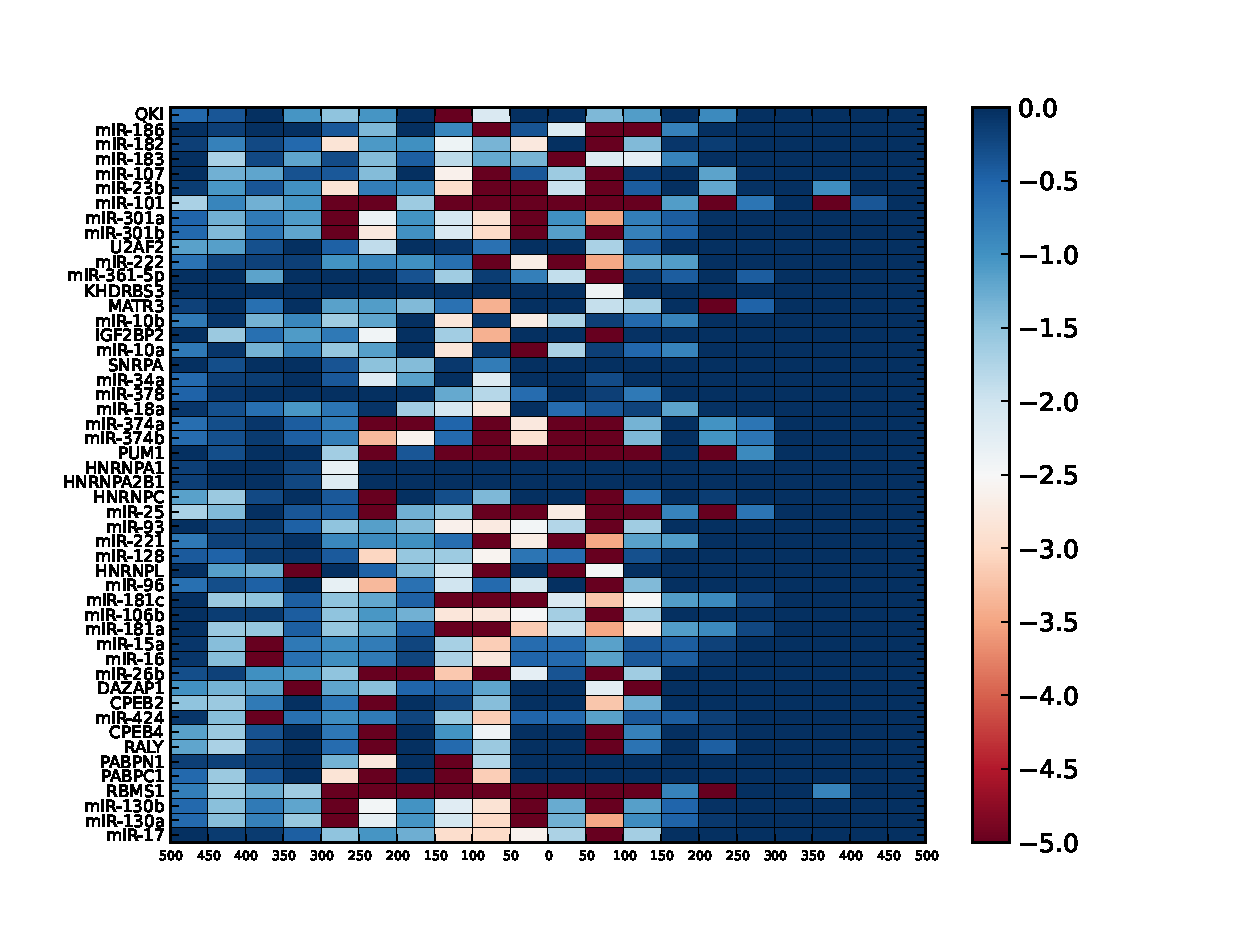
\includegraphics[width=0.9\textwidth]{appendix1/figures/PUM2_AUcontent_expressed_heatmap_qvalues1.eps}
   	\caption{Co-occurrence q-value heatmap plots of binding sites of PUM2 - AUcontent shuffle (Part 2)}
\end{figure}

\begin{figure}
   	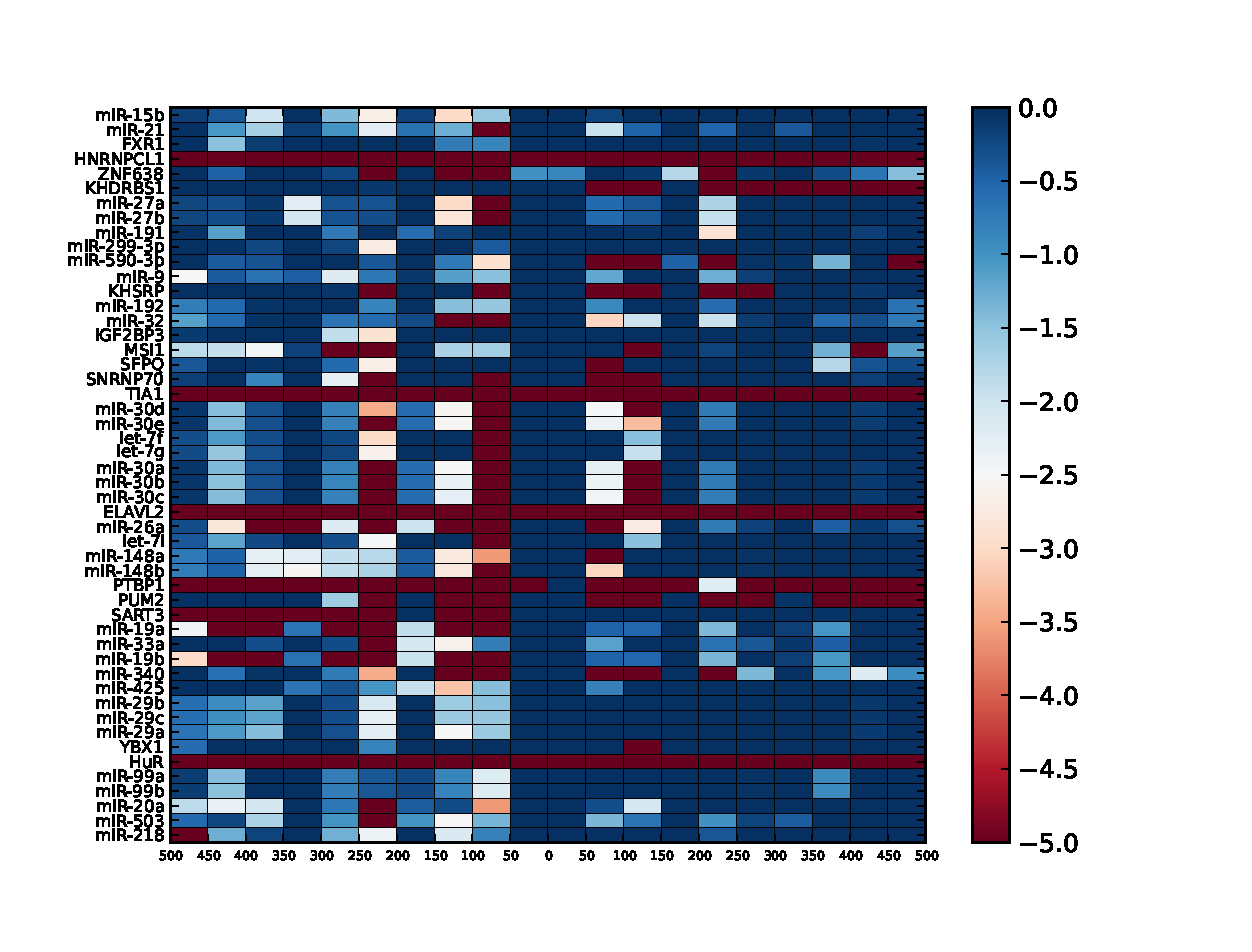
\includegraphics[width=0.9\textwidth,clip]{appendix1/figures/HuR_normal_expressed_heatmap_qvalues0.eps}
   	\caption{Co-occurrence q-value heatmap plots of binding sites of HuR - normal shuffle (Part 1)}
\end{figure}
\clearpage
\begin{figure}
   	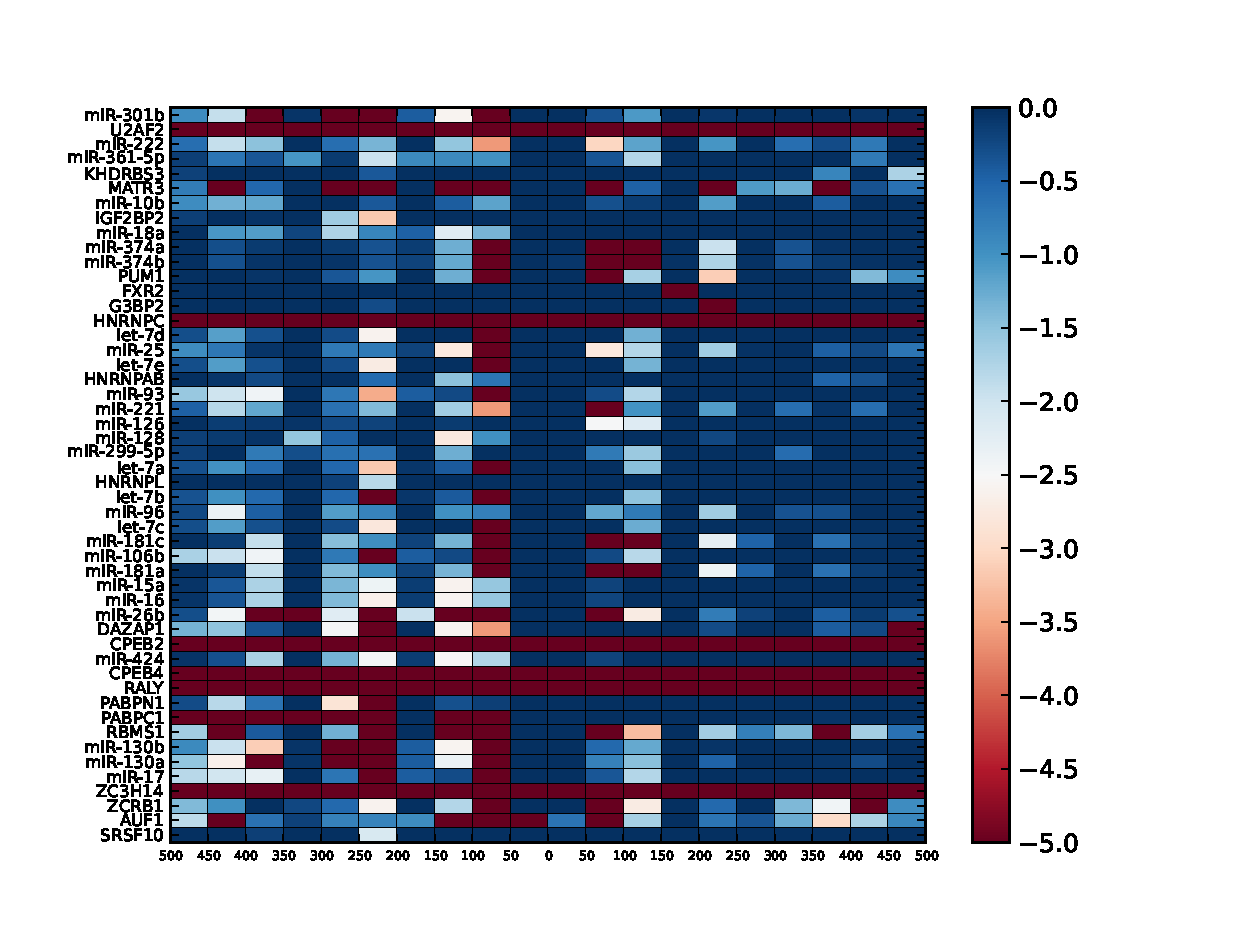
\includegraphics[width=0.9\textwidth]{appendix1/figures/HuR_normal_expressed_heatmap_qvalues1.eps}
   	\caption{Co-occurrence q-value heatmap plots of binding sites of HuR - normal shuffle (Part 2)}
\end{figure}

\begin{figure}
   	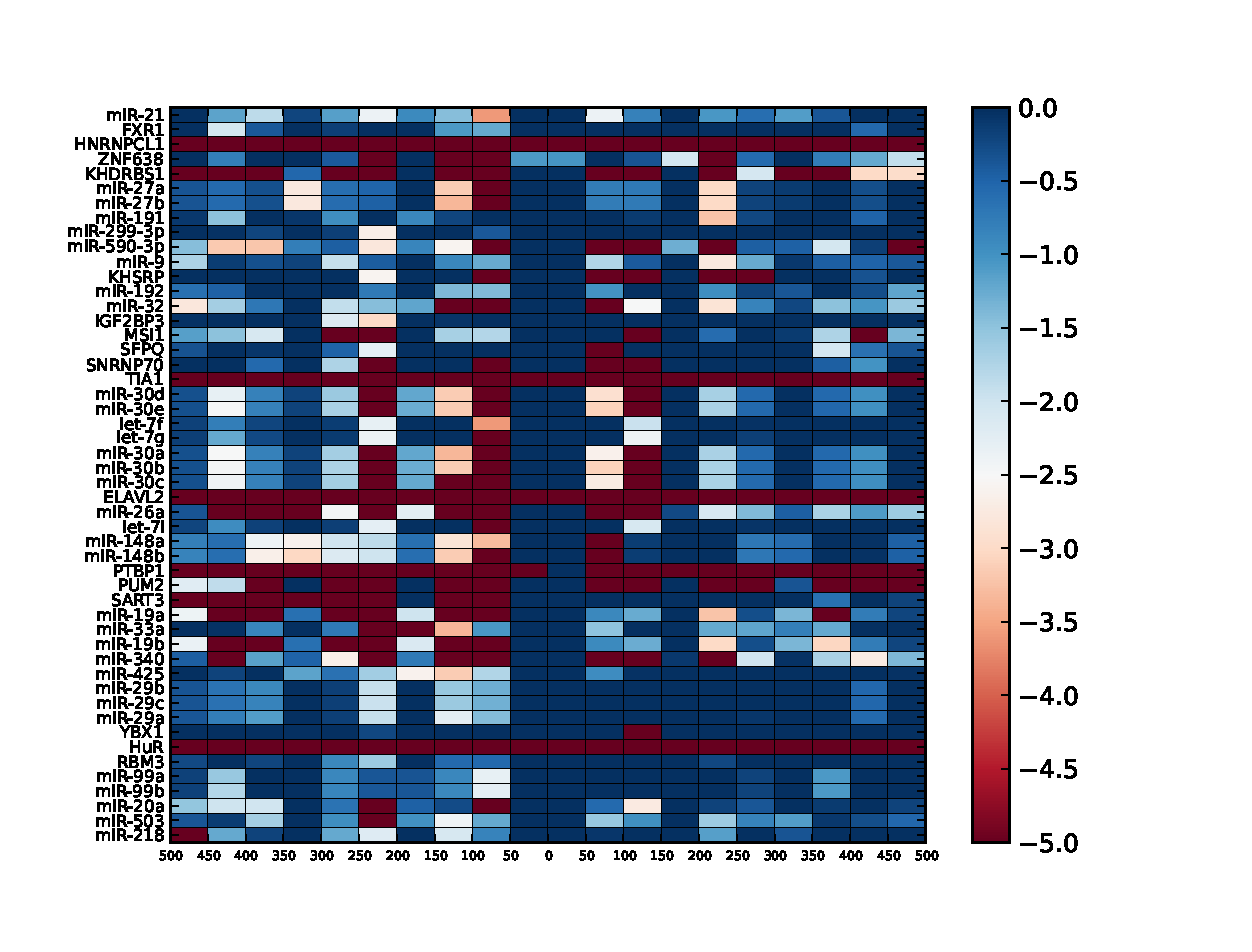
\includegraphics[width=0.9\textwidth]{appendix1/figures/HuR_decile_expressed_heatmap_qvalues0.eps}
   	\caption{Co-occurrence q-value heatmap plots of binding sites of HuR - decile shuffle (Part 1)}
\end{figure}
\clearpage
\begin{figure}
   	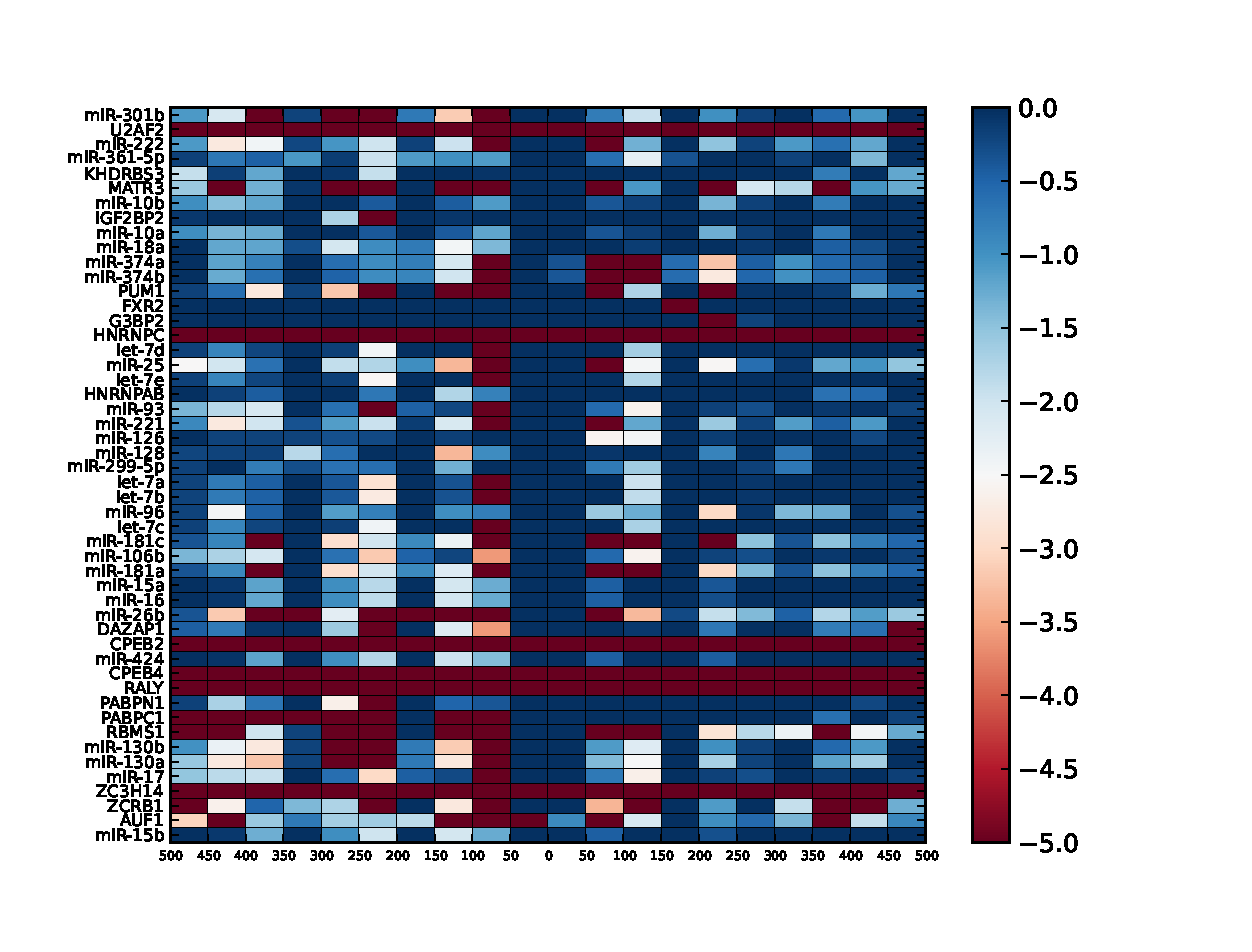
\includegraphics[width=0.9\textwidth,clip]{appendix1/figures/HuR_decile_expressed_heatmap_qvalues1.eps}
   	\caption{Co-occurrence q-value heatmap plots of binding sites of HuR - decile shuffle (Part 2)}
\end{figure}

\begin{figure}
   	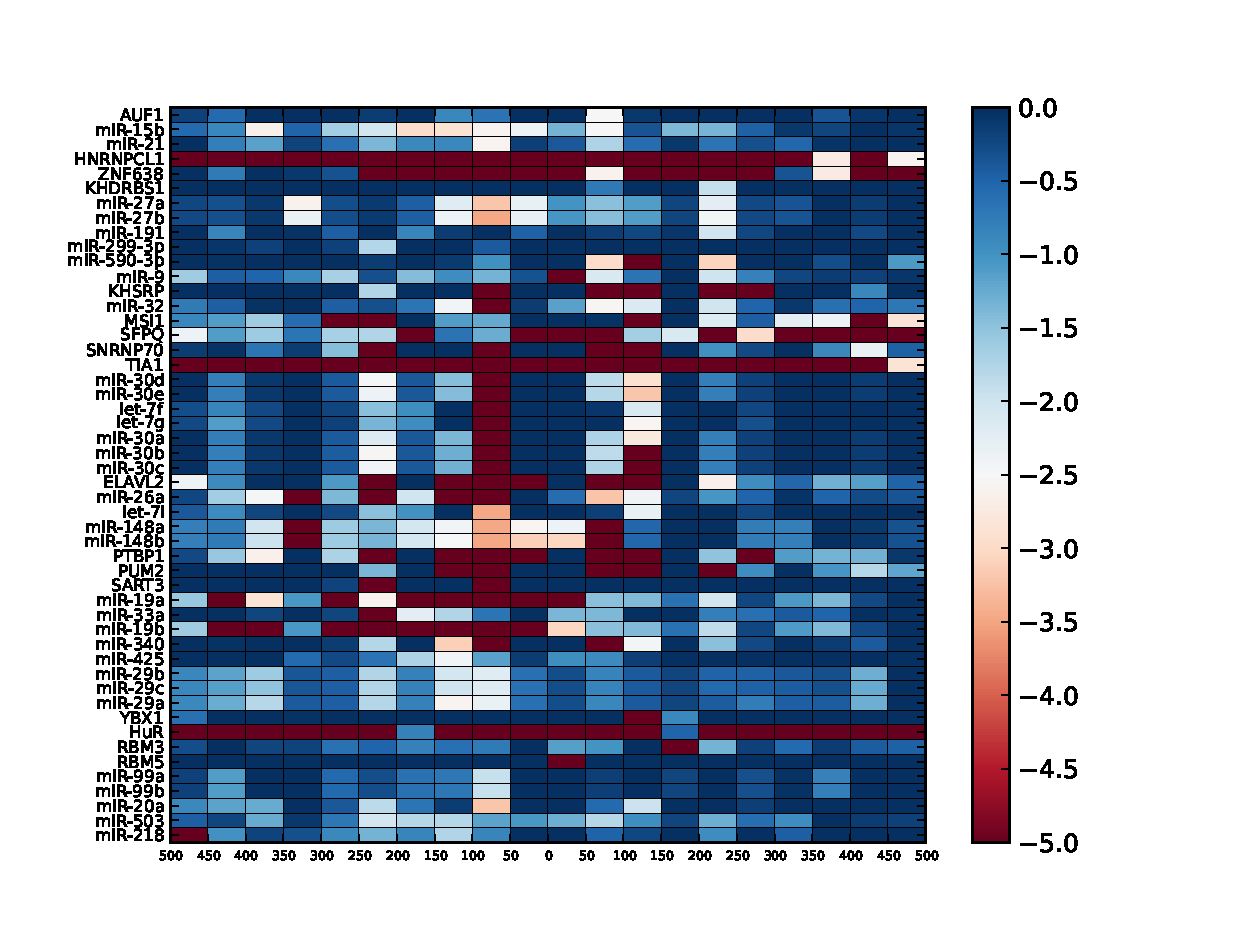
\includegraphics[width=0.9\textwidth]{appendix1/figures/HuR_AUcontent_expressed_heatmap_qvalues0.eps}
   	\caption{Co-occurrence q-value heatmap plots of binding sites of HuR - AUcontent shuffle (Part 1)}
\end{figure}
\clearpage
\begin{figure}
   	\includegraphics[width=0.9\textwidth]{appendix1/figures/HuR_AUcontent_expressed_heatmap_qvalues1.eps}
   	\caption{Co-occurrence q-value heatmap plots of binding sites of HuR - AUcontent shuffle (Part 2)}
\end{figure}

\begin{figure}
   	\includegraphics[width=0.9\textwidth]{appendix1/figures/IGF2BP2_normal_expressed_heatmap_qvalues0.eps}
   	\caption{Co-occurrence q-value heatmap plots of binding sites of IGF2BP2 - normal shuffle}
\end{figure}
\clearpage
\begin{figure}
   	\includegraphics[width=0.9\textwidth]{appendix1/figures/IGF2BP2_decile_expressed_heatmap_qvalues0.eps}
   	\caption{Co-occurrence q-value heatmap plots of binding sites of IGF2BP2 - decile shuffle}
\end{figure}

\begin{figure}
   	\includegraphics[width=0.9\textwidth]{appendix1/figures/IGF2BP2_AUcontent_expressed_heatmap_qvalues0.eps}
   	\caption{Co-occurrence q-value heatmap plots of binding sites of IGF2BP2 - AUcontent shuffle}
\end{figure}
\clearpage
\begin{figure}
   	\includegraphics[width=0.9\textwidth]{appendix1/figures/IGF2BP3_normal_expressed_heatmap_qvalues0.eps}
   	\caption{Co-occurrence q-value heatmap plots of binding sites of IGF2BP3 - normal shuffle}
\end{figure}

\begin{figure}
	\includegraphics[width=0.9\textwidth]{appendix1/figures/IGF2BP3_decile_expressed_heatmap_qvalues0.eps}
	\caption{Co-occurrence q-value heatmap plots of binding sites of IGF2BP3 - decile shuffle}
\end{figure}
\clearpage
\begin{figure}
   	\includegraphics[width=0.9\textwidth]{appendix1/figures/IGF2BP3_AUcontent_expressed_heatmap_qvalues0.eps}
   	\caption{Co-occurrence q-value heatmap plots of binding sites of IGF2BP3 - AUcontent shuffle}
\end{figure}

\begin{figure}
   	\includegraphics[width=0.9\textwidth]{appendix1/figures/PTBP1_AUcontent_expressed_heatmap_qvalues0.eps}
   	\caption{Co-occurrence q-value heatmap plots of binding sites of PTBP1 - normal shuffle}
\end{figure}
\clearpage
\begin{figure}
	\includegraphics[width=0.9\textwidth]{appendix1/figures/PTBP1_decile_expressed_heatmap_qvalues0.eps}
	\caption{Co-occurrence q-value heatmap plots of binding sites of PTBP1 - decile shuffle}
\end{figure}

\begin{figure}
	\includegraphics[width=0.9\textwidth]{appendix1/figures/PTBP1_AUcontent_expressed_heatmap_qvalues0.eps}
	\caption{Co-occurrence q-value heatmap plots of binding sites of PTBP1 - AUcontent shuffle}
\end{figure}
\clearpage
\begin{figure}
   	\includegraphics[width=0.9\textwidth]{appendix1/figures/HNRNPL_normal_expressed_heatmap_qvalues0.eps}
   	\caption{Co-occurrence q-value heatmap plots of binding sites of HNRNPL - decile shuffle}
\end{figure}

\begin{figure}
   	\includegraphics[width=0.9\textwidth]{appendix1/figures/HNRNPL_AUcontent_expressed_heatmap_qvalues0.eps}
   	\caption{Co-occurrence q-value heatmap plots of binding sites of HNRNPL - AUcontent shuffle}
\end{figure}
\newpage
\clearpage
\section{Co-occurrence q-value heatmap plots of miRNAs of interest}
\clearpage
\begin{figure}
   	\includegraphics[width=0.9\textwidth,clip]{appendix1/figures/let-7b_normal_expressed_heatmap_qvalues0.eps}
   	\caption{Co-occurrence q-value heatmap plots of binding sites of let-7b - normal shuffle}
\end{figure}

\begin{figure}
   	\includegraphics[width=0.9\textwidth,clip]{appendix1/figures/let-7b_decile_expressed_heatmap_qvalues0.eps}
   	\caption{Co-occurrence q-value heatmap plots of binding sites of let-7b - decile shuffle}
\end{figure}
\clearpage
\begin{figure}
   	\includegraphics[width=0.9\textwidth,clip]{appendix1/figures/let-7b_AUcontent_expressed_heatmap_qvalues0.eps}
   	\caption{Co-occurrence q-value heatmap plots of binding sites of let-7b - AUcontent shuffle}
\end{figure}

\begin{figure}
   	\includegraphics[width=0.9\textwidth,clip]{appendix1/figures/miR-9_normal_expressed_heatmap_qvalues0.eps}
   	\caption{Co-occurrence q-value heatmap plots of binding sites of miR-9 - normal shuffle}
\end{figure}
\clearpage
\begin{figure}
   	\includegraphics[width=0.9\textwidth,clip]{appendix1/figures/miR-9_decile_expressed_heatmap_qvalues0.eps}
   	\caption{Co-occurrence q-value heatmap plots of binding sites of miR-9 - decile shuffle}
\end{figure}

\begin{figure}
   	\includegraphics[width=0.9\textwidth,clip]{appendix1/figures/miR-9_AUcontent_expressed_heatmap_qvalues0.eps}
   	\caption{Co-occurrence q-value heatmap plots of binding sites of miR-9 - AUcontent shuffle}
\end{figure}
\clearpage
\begin{figure}
   	\includegraphics[width=0.9\textwidth,clip]{appendix1/figures/miR-15a_normal_expressed_heatmap_qvalues0.eps}
   	\caption{Co-occurrence q-value heatmap plots of binding sites of miR-15a - normal shuffle}
\end{figure}

\begin{figure}
   	\includegraphics[width=0.9\textwidth,clip]{appendix1/figures/miR-15a_decile_expressed_heatmap_qvalues0.eps}
   	\caption{Co-occurrence q-value heatmap plots of binding sites of miR-15a - decile shuffle}
\end{figure}
\clearpage
\begin{figure}
   	\includegraphics[width=0.9\textwidth,clip]{appendix1/figures/miR-15a_AUcontent_expressed_heatmap_qvalues0.eps}
   	\caption{Co-occurrence q-value heatmap plots of binding sites of miR-15a - AUcontent shuffle (Part 1)}
\end{figure}

\begin{figure}
   	\includegraphics[width=0.9\textwidth,clip]{appendix1/figures/miR-15a_AUcontent_expressed_heatmap_qvalues1.eps}
   	\caption{Co-occurrence q-value heatmap plots of binding sites of miR-15a - AUcontent shuffle (Part 2)}
\end{figure}
\clearpage
\begin{figure}
   	\includegraphics[width=0.9\textwidth,clip]{appendix1/figures/miR-16_normal_expressed_heatmap_qvalues0.eps}
   	\caption{Co-occurrence q-value heatmap plots of binding sites of miR-16 - normal shuffle}
\end{figure}

\begin{figure}
   	\includegraphics[width=0.9\textwidth,clip]{appendix1/figures/miR-16_decile_expressed_heatmap_qvalues0.eps}
   	\caption{Co-occurrence q-value heatmap plots of binding sites of miR-16 - decile shuffle}
\end{figure}
\clearpage
\begin{figure}
   	\includegraphics[width=0.9\textwidth,clip]{appendix1/figures/miR-16_AUcontent_expressed_heatmap_qvalues0.eps}
   	\caption{Co-occurrence q-value heatmap plots of binding sites of miR-16 - AUcontent shuffle}
\end{figure}

\begin{figure}
   	\includegraphics[width=0.9\textwidth,clip]{appendix1/figures/miR-34a_normal_expressed_heatmap_qvalues0.eps}
   	\caption{Co-occurrence q-value heatmap plots of binding sites of miR-34a - normal shuffle}
\end{figure}
\clearpage
\begin{figure}
   	\includegraphics[width=0.9\textwidth,clip]{appendix1/figures/miR-34a_AUcontent_expressed_heatmap_qvalues0.eps}
   	\caption{Co-occurrence q-value heatmap plots of binding sites of miR-34a - AUcontent shuffle}
\end{figure}

\begin{figure}
	\includegraphics[width=0.9\textwidth,clip]{appendix1/figures/miR-106b_normal_expressed_heatmap_qvalues0.eps}
	\caption{Co-occurrence q-value heatmap plots of binding sites of miR-106b - normal shuffle}
\end{figure}
\clearpage
\begin{figure}
	\includegraphics[width=0.9\textwidth,clip]{appendix1/figures/miR-106b_decile_expressed_heatmap_qvalues0.eps}
	\caption{Co-occurrence q-value heatmap plots of binding sites of miR-106b - decile shuffle}
\end{figure}

\begin{figure}
	\includegraphics[width=0.9\textwidth,clip]{appendix1/figures/miR-106b_AUcontent_expressed_heatmap_qvalues0.eps}
	\caption{Co-occurrence q-value heatmap plots of binding sites of miR-106b - AUcontent shuffle}
\end{figure}
\clearpage
\begin{figure}
   	\includegraphics[width=0.9\textwidth,clip]{appendix1/figures/miR-148b_normal_expressed_heatmap_qvalues0.eps}
   	\caption{Co-occurrence q-value heatmap plots of binding sites of miR-148b - normal shuffle}
\end{figure}

\begin{figure}
   	\includegraphics[width=0.9\textwidth,clip]{appendix1/figures/miR-148b_decile_expressed_heatmap_qvalues0.eps}
   	\caption{Co-occurrence q-value heatmap plots of binding sites of miR-148b - decile shuffle}
\end{figure}
\clearpage
\begin{figure}
   	\includegraphics[width=0.9\textwidth,clip]{appendix1/figures/miR-148b_AUcontent_expressed_heatmap_qvalues0.eps}
   	\caption{Co-occurrence q-value heatmap plots of binding sites of miR-148b - AUcontent shuffle}
\end{figure}

\begin{figure}
   	\includegraphics[width=0.9\textwidth,clip]{appendix1/figures/miR-181a_normal_expressed_heatmap_qvalues0.eps}
   	\caption{Co-occurrence q-value heatmap plots of binding sites of miR-181a - normal shuffle (Part 1)}
\end{figure}
\clearpage
\begin{figure}
   	\includegraphics[width=0.9\textwidth,clip]{appendix1/figures/miR-181a_normal_expressed_heatmap_qvalues1.eps}
   	\caption{Co-occurrence q-value heatmap plots of binding sites of miR-181a - normal shuffle (Part 2)}
\end{figure}

\begin{figure}
   	\includegraphics[width=0.9\textwidth,clip]{appendix1/figures/miR-181a_decile_expressed_heatmap_qvalues0.eps}
   	\caption{Co-occurrence q-value heatmap plots of binding sites of miR-181a - decile shuffle (Part 1)}
\end{figure}
\clearpage
\begin{figure}
   	\includegraphics[width=0.9\textwidth,clip]{appendix1/figures/miR-181a_decile_expressed_heatmap_qvalues1.eps}
   	\caption{Co-occurrence q-value heatmap plots of binding sites of miR-181a - decile shuffle (Part 2)}
\end{figure}

\begin{figure}
   	\includegraphics[width=0.9\textwidth,clip]{appendix1/figures/miR-181a_AUcontent_expressed_heatmap_qvalues0.eps}
   	\caption{Co-occurrence q-value heatmap plots of binding sites of miR-181a - AUcontent shuffle (Part 1)}
\end{figure}
\clearpage
\begin{figure}
   	\includegraphics[width=0.9\textwidth,clip]{appendix1/figures/miR-181a_AUcontent_expressed_heatmap_qvalues1.eps}
   	\caption{Co-occurrence q-value heatmap plots of binding sites of miR-181a - AUcontent shuffle (Part 2)}
\end{figure}
%\shorthandon{=}
%
% If you are a Ph.D. Student you need to insert a CV at the end of you thesis
% Check vita.tex for a simple CV template in Latex

\end{document}
